%%%%%%%%%%%%%%%%%%%%%%%%%%%%%%%%%%%%%%%%%
% Masters/Doctoral Thesis 
% LaTeX Template
% Version 2.3 (25/3/16)
%
% This template has been downloaded from:
% http://www.LaTeXTemplates.com
%
% Version 2.x major modifications by:
% Vel (vel@latextemplates.com)
%
% This template is based on a template by:
% Steve Gunn (http://users.ecs.soton.ac.uk/srg/softwaretools/document/templates/)
% Sunil Patel (http://www.sunilpatel.co.uk/thesis-template/)
%
% Template license:
% CC BY-NC-SA 3.0 (http://creativecommons.org/licenses/by-nc-sa/3.0/)
%
%%%%%%%%%%%%%%%%%%%%%%%%%%%%%%%%%%%%%%%%%

%% Note: To include the bibliography -> run pdflatex main.tex > bibtex main.aux > pdflatex main.tex > pdflatex main.tex

%----------------------------------------------------------------------------------------
%	PACKAGES AND OTHER DOCUMENT CONFIGURATIONS
%----------------------------------------------------------------------------------------

\documentclass[
  12pt, % The default document font size, options: 10pt, 11pt, 12pt
  twoside, % Two side (alternating margins) for binding by default, uncomment to switch to one side
  %chapterinoneline,% Have the chapter title next to the number in one single line
  english, % ngerman for German
  onehalfspacing, % Single line spacing, alternatives: singlespacing, onehalfspacing or doublespacing
  %draft, % Uncomment to enable draft mode (no pictures, no links, overfull hboxes indicated)
  %nolistspacing, % If the document is onehalfspacing or doublespacing, uncomment this to set spacing in lists to single
  %liststotoc, % Uncomment to add the list of figures/tables/etc to the table of contents
  %toctotoc, % Uncomment to add the main table of contents to the table of contents
  %parskip, % Uncomment to add space between paragraphs
  %nohyperref, % Uncomment to not load the hyperref package
  %headsepline, % Uncomment to get a line under the header
]{setting} % The class file specifying the document structure

\usepackage{verbatim}
\usepackage[utf8]{inputenc} % Required for inputting international characters
\usepackage[T1]{fontenc} % Output font encoding for international characters
\usepackage{palatino} % Use the Palatino font by default
\usepackage[backend=bibtex,style=numeric-comp,sorting=none,natbib=true]{biblatex} % Use the bibtex backend with the authoryear citation style (which resembles APA)
\addbibresource{main.bib} % The filename of the bibliography
\usepackage[autostyle=true]{csquotes} % Required to generate language-dependent quotes in the bibliography
\usepackage{multirow}
\usepackage{mathrsfs}
\usepackage{amssymb}
\usepackage{amsmath}
\usepackage{pgfmath}
\usepackage{pgffor}
\usepackage{pdflscape}
\usepackage{rotating}
\usepackage{lineno}
\usepackage{enumitem}
\usepackage{courier}
\usepackage{booktabs}
\usepackage{afterpage}
\usepackage{xspace}
\usepackage{hhline}
\usepackage{braket}
\usepackage[final]{pdfpages}
% \usepackage{hyperref}
\usepackage{CJKutf8}



% \captionsetup{justification=raggedright, singlelinecheck=false, format=hang}
\captionsetup{margin=0cm, justification=raggedright, singlelinecheck=true, format=plain}

\renewcommand{\arraystretch}{1.2}
\DeclareMathOperator{\erf}{erf}

\newcommand{\pT}{\ensuremath{p_{T}}\xspace}
\newcommand{\PT}{\ensuremath{p_{T}}\xspace}
\newcommand{\Mx}{\ensuremath{\tilde{M_{X}}}\xspace}
\newcommand{\Hgg}{\ensuremath{H\to\gamma\gamma}\xspace}
\newcommand{\Hbb}{\ensuremath{H\to b\bar{b}}\xspace}
\newcommand{\ttbar}{\ensuremath{t\bar{t}}\xspace}
\newcommand{\HH}{\ensuremath{HH}\xspace}
\newcommand{\Z}{\ensuremath{Z}\xspace}
\newcommand{\GeV}{GeV}
% \newcommand{\ell}{\ensuremath{ll}}
\newcommand{\bbgg}{\ensuremath{b\bar{b}\gamma\gamma}\xspace}
% \newcommand{\gg}{\ensuremath{\gamma\gamma}\xspace}
\newcommand{\HHbbgg}{\ensuremath{HH\to b\bar{b}\gamma\gamma}\xspace}
\newcommand{\bbbb}{\ensuremath{b\bar{b}b\bar{b}}\xspace}
\newcommand{\DR}{\ensuremath{\Delta R}\xspace}
% \newcommand{\MET}{\ensuremath{E_{T}^{miss}}\xspace}
\newcommand{\MET}{MET\xspace}
\newcommand{\Mgg}{\ensuremath{m_{\gamma\gamma}}\xspace}
\newcommand{\Mjj}{\ensuremath{m_{\rm jj}}\xspace}

\newcommand\blankpage{
  \null
  \thispagestyle{empty}
  \addtocounter{page}{-1}
  \newpage
}

%----------------------------------------------------------------------------------------
%	MARGIN SETTINGS
%----------------------------------------------------------------------------------------

\geometry{
  paper=a4paper, % Change to letterpaper for US letter
  inner=2.0cm, % Inner margin 2.5cm
  outer=2.2cm, % Outer margin 3.8cm
  bindingoffset=2cm, % Binding offset
  top=1.5cm, % Top margin
  bottom=1.5cm, % Bottom margin
  %showframe,% show how the type block is set on the page
}

%----------------------------------------------------------------------------------------
%	THESIS INFORMATION
%----------------------------------------------------------------------------------------

\thesistitle{Search for the production of two Higgs bosons in the final state with two photons and two b quarks in proton-proton collision at $\sqrt{s}$ = 13 TeV} % Your thesis title, this is used in the title and abstract, print it elsewhere with \ttitle
\supervisor{Kuo, Chia-Ming} % Your supervisor's name, this is used in the title page, print it elsewhere with \supname
\examiner{Kao, Chung Wen} % Your examiner's name, this is not currently used anywhere in the template, print it elsewhere with \examname
\degree{Master of Physics} % Your degree name, this is used in the title page and abstract, print it elsewhere with \degreename
\author{Yeh, Cheng-Wei} % Your name, this is used in the title page and abstract, print it elsewhere with \authorname
%\addresses{} % Your address, this is not currently used anywhere in the template, print it elsewhere with \addressname
%\subject{Physical Sciences} % Your subject area, this is not currently used anywhere in the template, print it elsewhere with \subjectname
%\keywords{} % Keywords for your thesis, this is not currently used anywhere in the template, print it elsewhere with \keywordnames
\university{National Central University} % Your university's name and URL, this is used in the title page and abstract, print it elsewhere with \univname
\department{Department of Physics} % Your department's name and URL, this is used in the title page and abstract, print it elsewhere with \deptname
%\group{High Energy Physics Experiment} % Your research group's name and URL, this is used in the title page, print it elsewhere with \groupname
%\faculty{} % Your faculty's name and URL, this is used in the title page and abstract, print it elsewhere with \facname

\hypersetup{pdftitle=\ttitle} % Set the PDF's title to your title
\hypersetup{pdfauthor=\authorname} % Set the PDF's author to your name
%\hypersetup{pdfkeywords=\keywordnames} % Set the PDF's keywords to your keywords

\begin{document}

\frontmatter % Use roman page numbering style (i, ii, iii, iv...) for the pre-content pages
\pagestyle{plain} % Default to the plain heading style until the thesis style is called for the body content

\afterpage{\blankpage} % Add a new blank page without page number
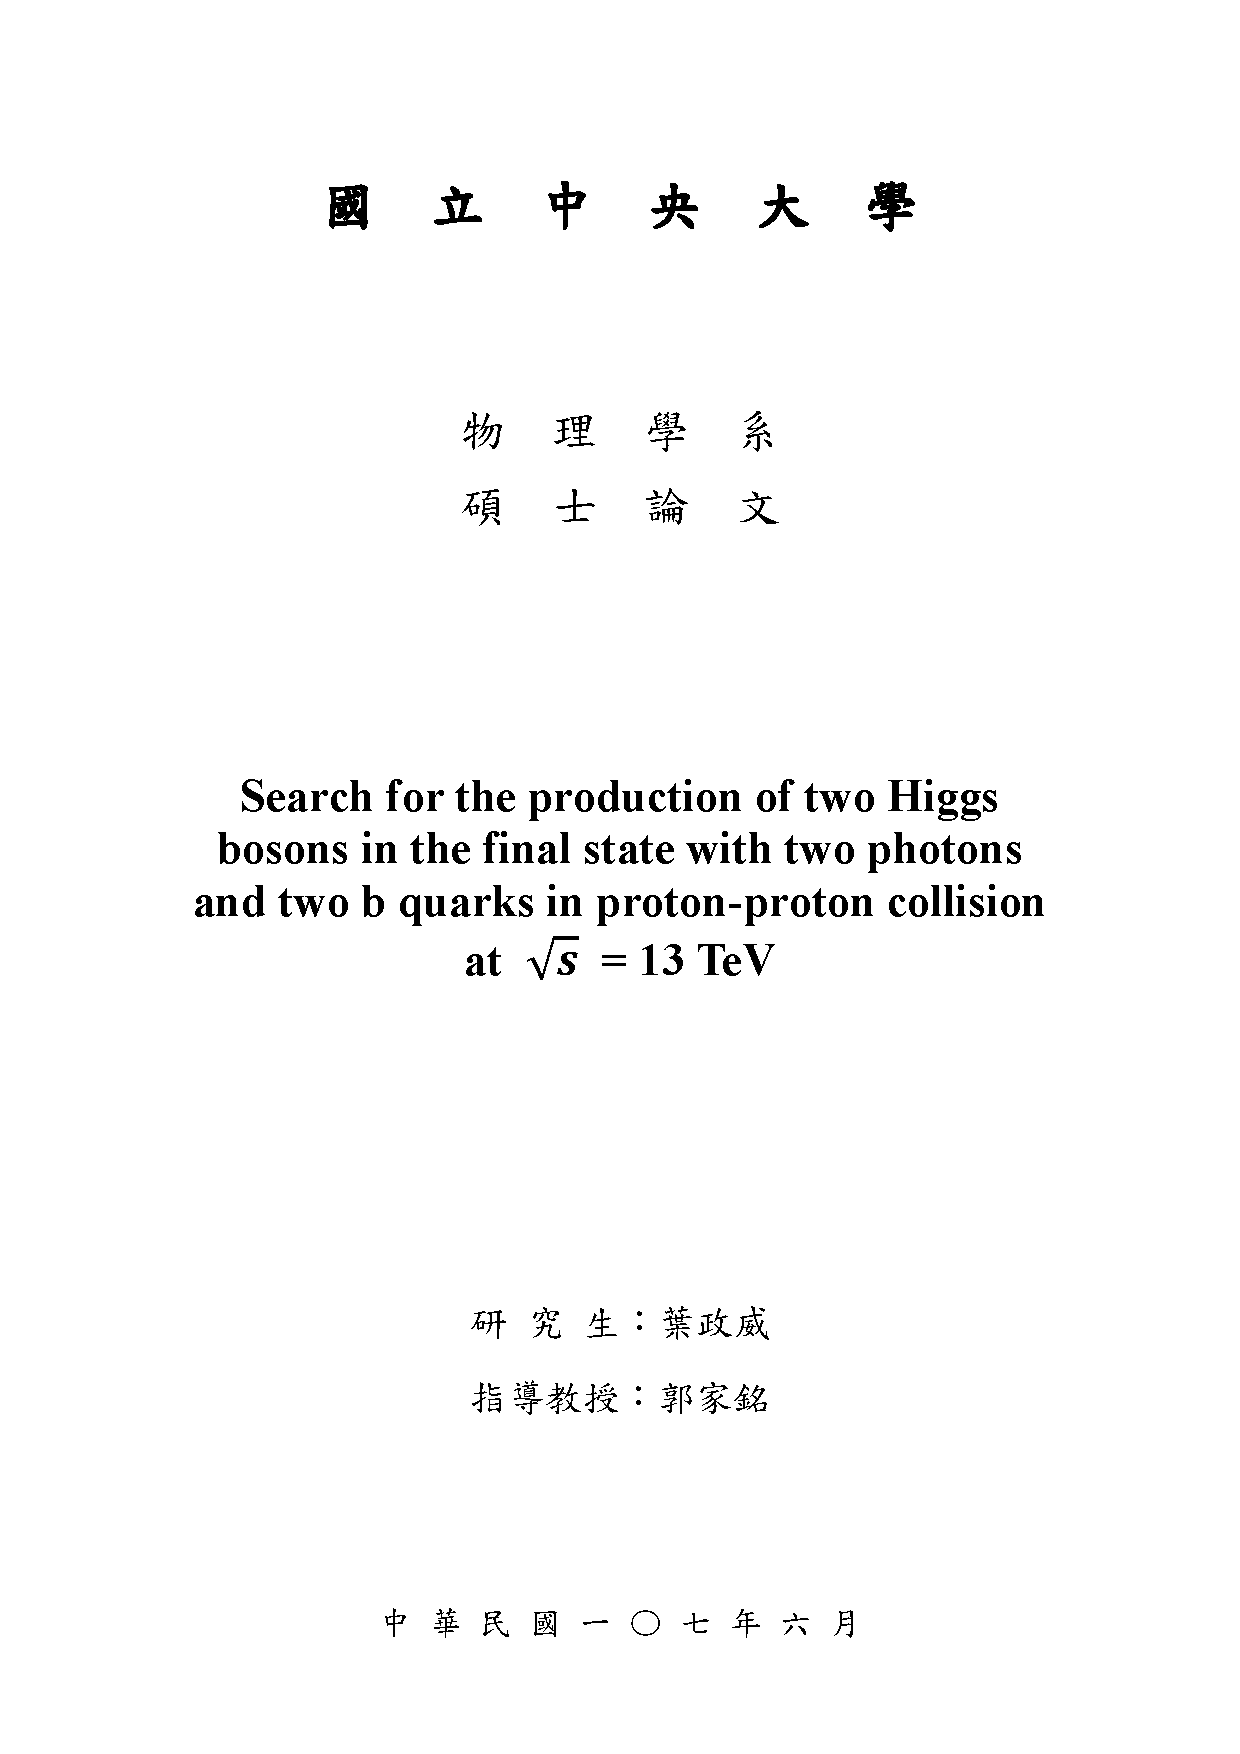
\includepdf{cover2.pdf}

\afterpage{\blankpage}
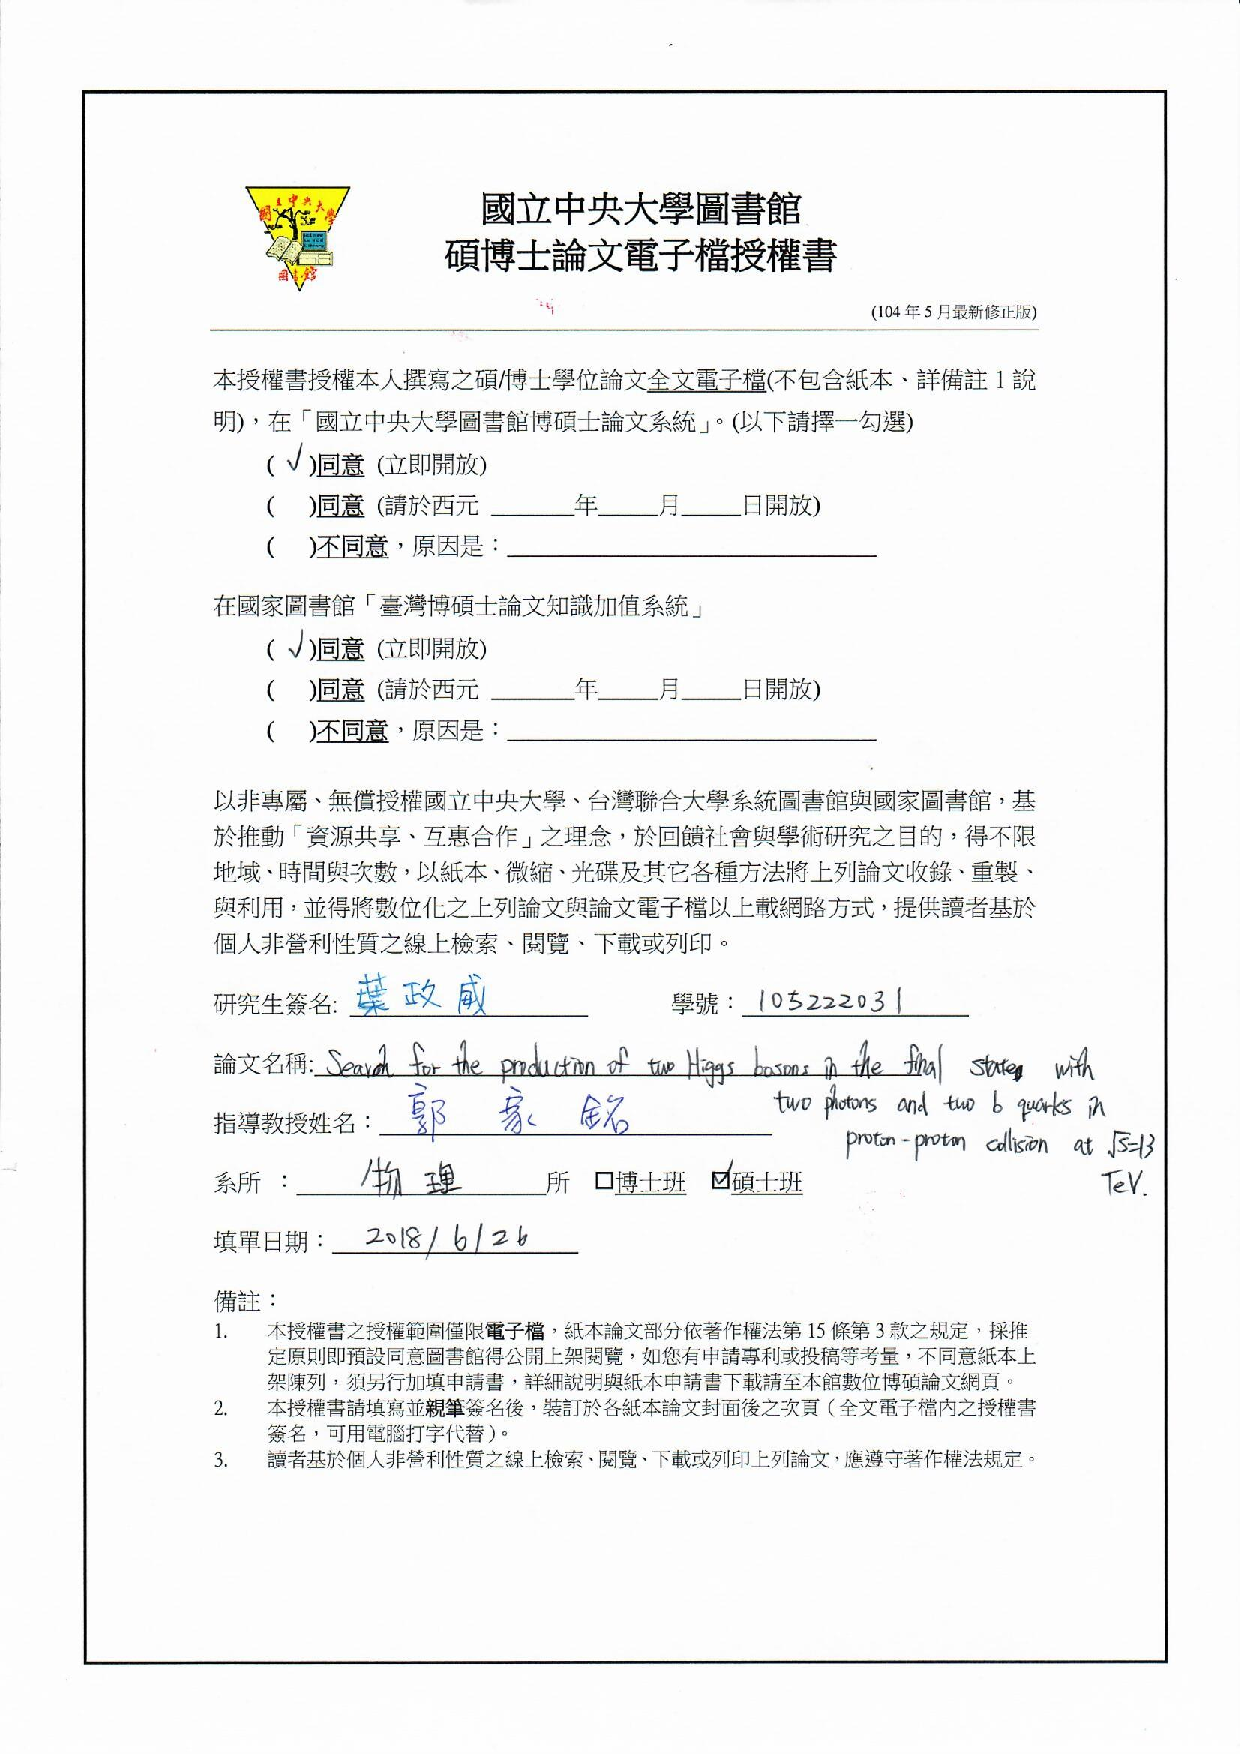
\includepdf{OralPage_1.pdf}

\afterpage{\blankpage}
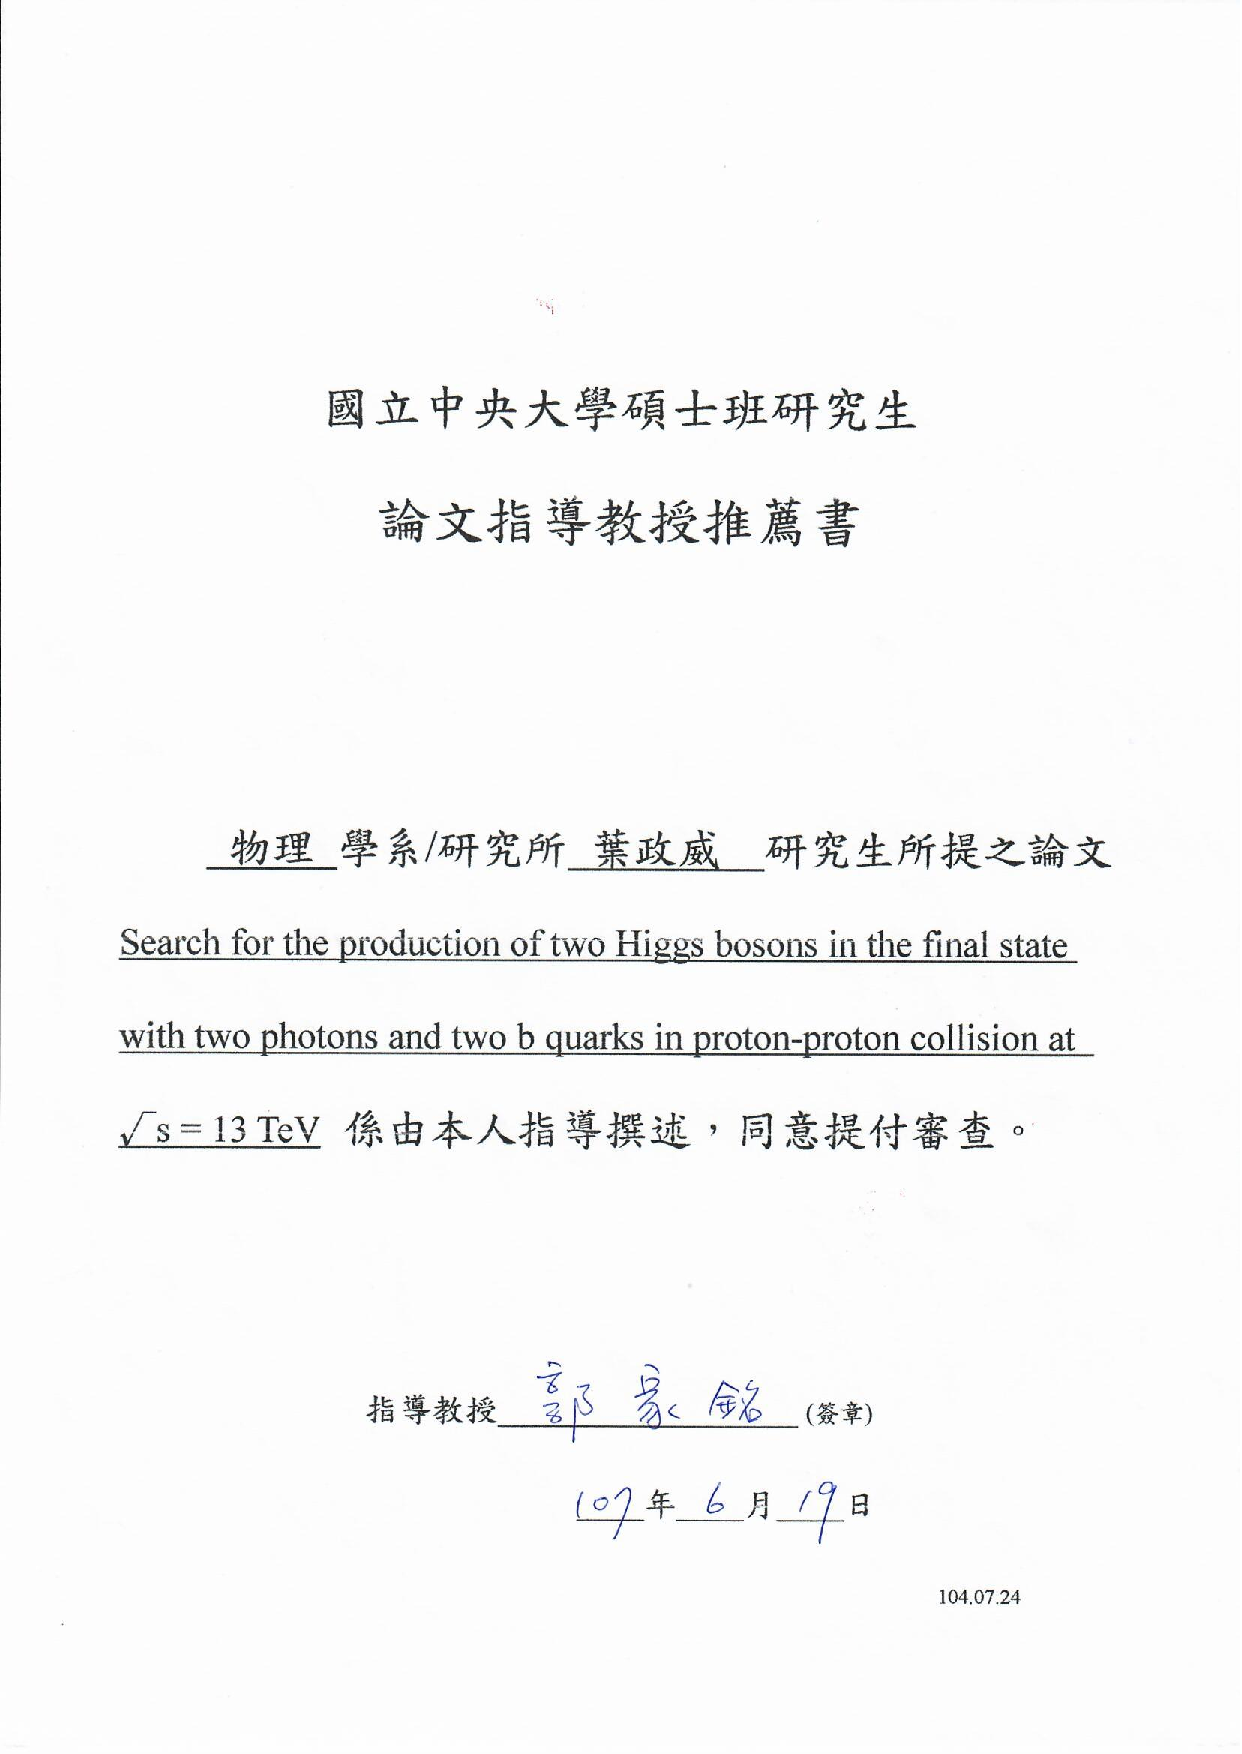
\includepdf{OralPage_2.pdf}

\afterpage{\blankpage}
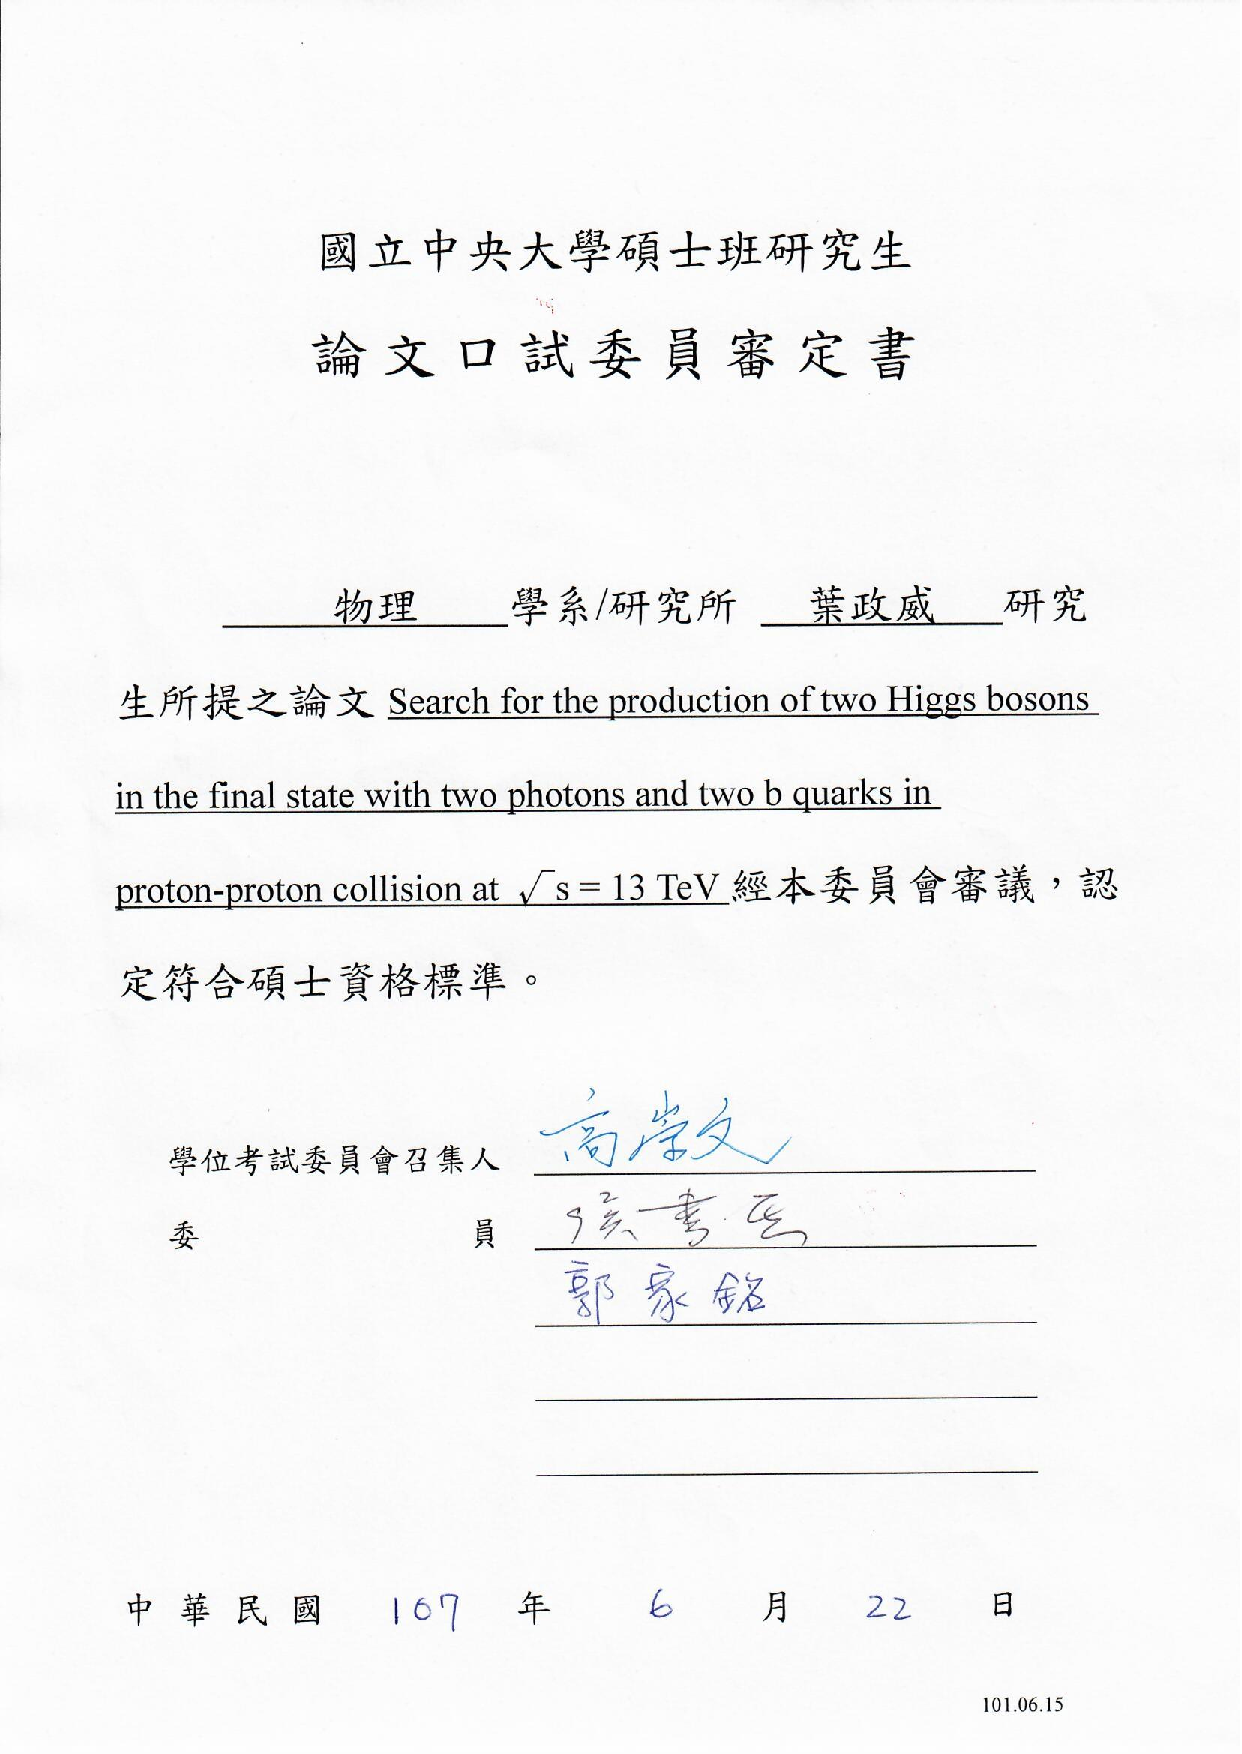
\includepdf{OralPage_3.pdf}





%----------------------------------------------------------------------------------------
%	TITLE PAGE
%----------------------------------------------------------------------------------------

\begin{titlepage}
  \begin{center} \setstretch{1.15}
    {\Large \bfseries \ttitle \par}
    \bigskip
    {\normalsize by \par}
    \bigskip
    {\large \authorname \par}
    \bigskip
    {\normalsize Submitted to the \deptname \par in partial fulfillment of the requirements for the degree of \par}
    \bigskip
    {\large \degreename \par}
    \bigskip    
    {at the \par}
    \bigskip
    {\large \MakeUppercase{\univname} \par}
    \bigskip
    {\normalsize June 2018 \par}
    \bigskip
    {\textcopyright \space \univname \space 2018. All rights reserved. \par}
    \bigskip \bigskip \bigskip 
    \begin{flushleft}
      {\large Author \dotfill \par}
    \end{flushleft}
    \begin{flushright} 
      {\deptname \par \today \par}
    \end{flushright}
    \begin{flushleft}
      {\large Certified by \dotfill \par}
    \end{flushleft}
    \begin{flushright} 
      {\supname \par Associate Professor \par Thesis Supervisor \par}
    \end{flushright}
    % \begin{flushleft}
      % {\large Accepted by \dotfill \par}
    % \end{flushleft}
    % \begin{flushright} 
      % {\examname \par Professor \par Chairman, Thesis Committee \par}
    % \end{flushright}
  \end{center}
\end{titlepage}

%\cleardoublepage

%----------------------------------------------------------------------------------------
%	ABSTRACT PAGE
%----------------------------------------------------------------------------------------

\begin{abstract} \setstretch{1.15}
%  \addchaptertocentry{\abstractname} % Add the abstract to the table of contents

  \noindent{\large \textbf{Abstract} \par}
  \bigskip
  \noindent{
  % The production of a pair of Higgs bosons is a rare process in proton-proton collisions.
  % There are two kinds of production.
  % One is that the Standard Model (SM) predicts that the Higgs boson pairs can be from Higgs self-interactions, which called non-resonant process.
  % This process can help us to understand the Higgs self-coupling constant and the structure of Higgs scalar potential field.
  % Another one is predicted by many theories beyond the SM.
  % There are some kinds of new particles which can decay into two Higgs and form the resonance peak in the mass spectrum of di-Higgs.
  % Two decay channels are used in this study: $H\rightarrow$ $bb$ with high branching ratio and $H\rightarrow \gamma \gamma$ with good energy resolution.
  The search is presented for the production of a pair of Higgs bosons in the final state with two photons and two b quarks by full 2016 data, which corresponds to an integrated luminosity of 35.9 $fb^{-1}$ recorded by the CMS detector.
  Both resonant and non-resonant processes are investigated for the Standard Model (SM) and the Beyond the Standard Model (BSM) theories.
  The non-resonant production helps us to understand the Higgs field structure in the SM and other possible effects from BSMs.
  The resonant production is predicted by many BSMs. In this thesis, the hypothesis with the spin-0 and spin-2 new heavy particles which can decay into two Higgs bosons is searched and compared with the prediction from the warped extra dimension theory.
  The b-jet energy regression specifically developed for this analysis are employed to improve the sensitivity about 10\%.
  The observed results agree with the standard model prediction, and the limits on the exclusion of the BSM productions are also set.
  \par}
  \bigskip
  \noindent{Thesis Supervisor: \space \supname \par}
  \noindent{Title: \space Associate Professor \par}
  
\end{abstract}
% \afterpage{\blankpage}


\begin{CJK}{UTF8}{bkai}

\setstretch{1.25}
\checktoopen
\thispagestyle{plain}
\begin{center}
{\Huge \bfseries 摘 要 \par}
\end{center}
\bigskip
\bigskip
\bigskip
\bigskip
{\Large 

 本篇論文旨在尋找於質子–質子對撞下產生的雙希格斯粒子,分別衰變至一對光子及一對底夸克。
本分析使用了於2016年由大強子對撞機(LHC)產生的質子–質子對撞,總能量為$\sqrt{s}=13$ TeV,並由緊湊緲子線圈(CMS)所記錄,總亮度達到$35.9~fb^{-1}$。
此研究基於標準模型以及超越標準模型的理論,同時尋找非共振衰變的雙希格斯粒子以及由新粒子衰變的雙希格斯粒子。
非共振衰變可用於驗證希格斯機制以及探索其他可能的希格斯粒子與其他粒子的交互作用。
多維度模型預測了兩種與重力相關的新粒子,且這些新粒子可衰變到雙希格斯粒子。
本研究使用機器學習來輔助重建來自底夸克的強子噴流能量,使預測的生產截面的信心水準上限下降百分之十,達到更佳的結果。
本研究沒有觀察到顯著的訊號事件,並提供了實驗上對理論參數以及新粒子重量的限制區間。

\par}


\end{CJK}




\begin{CJK}{UTF8}{bkai}

\setstretch{1.25}
\checktoopen
\thispagestyle{plain}
\begin{center}
{\Huge \bfseries 致 謝 \par}
\end{center}
\bigskip
\bigskip
\bigskip
\bigskip
{\large 

 感謝指導教授郭家銘老師帶領我走過這四年的高能物理研究生活,教導我研究所需的技能以及知識,給予我出國參與國際團隊的機會,讓我得以一窺實驗高能物理研究的面貌。同時也感謝口試委員,讓這本論文得以完成。

 感謝系上的老師們教導眾多的物理知識,讓我學會更多物理工具以及開拓高能物理領域之外的眼界。

 感謝系辦的工作人員們以及高能實驗室助理張惠虹小姐協助處理繁瑣的手續,讓各項流程完美運轉。

 感謝這段期間在高能物理實驗研究團隊的成員:
Maxim\\、Andrey、Shilpi、Hien、Hoa、Victoria、Pocholo、Adam、張佑祥、張秋萍、曾師彥、杜仲倫、劉為尹,以及好勝的八加九們:汪本璿、鄭皓仁、賴培築、李明晏、張用威、童宇軒、劉書孝、徐郁瑜、葉智翔、張峻堯。謝謝你們在研究中提供種種助力,以及在上課、研究之餘陪我玩。

 感謝好同學們:蔡伯罕、蘇丰彥、王奕惟、藍亭奕、曾柏穎、馮思賢,以及熱音社的夥伴們,陪我玩、吵架、交換各種資訊、玩音樂,衝表演等,讓我的生活多采多姿。

 最後感謝我的家人,提供我經濟後盾以及精神支持,讓我得以完成學業。

 一百萬個感謝!
	

\par}


\end{CJK}



%----------------------------------------------------------------------------------------
%	LIST OF CONTENTS/FIGURES/TABLES PAGES
%----------------------------------------------------------------------------------------

\tableofcontents % Prints the main table of contents
% \listoffigures % Prints the list of figures
% \listoftables % Prints the list of tables

%----------------------------------------------------------------------------------------
%	THESIS CONTENT - CHAPTERS
%----------------------------------------------------------------------------------------

\mainmatter % Begin numeric (1,2,3...) page numbering
\pagestyle{thesis} % Return the page headers back to the "thesis" style

% Include the chapters of the thesis as separate files from the Chapters folder
% Uncomment the lines as you write the chapters

% \begin{linenumbers} %Turn line numbers on unless it is the final version
  
  \chapter{Introduction} % Main chapter title

\label{Chapter1} % Change X to a consecutive number; for referencing this chapter elsewhere, use \ref{ChapterX}

%----------------------------------------------------------------------------------------
%	SECTION 1
%----------------------------------------------------------------------------------------

\section{Introduction}

The discovery of new boson with mass around 125 GeV at the Large Hadron Collider (LHC) by the CMS~\cite{1207.7235} and ATLAS~\cite{1207.7214} opened a new era of particle physics.
The measured properties of this new particle are consistent with the Higgs boson in the Standard Model within the uncertainties.~\cite{1606.02266}
In the Standard Model (SM), the Higgs mechanism involves Higgs potential field to solve the mass problem of the gauge bosons and the fermions. % ** need to be fixed!
% There are two free parameters to describe the Higgs potential: mass of Higgs boson and its self-coupling constant. 
With the determined Higgs mass value, the structure of the Higgs potential field and the Higgs self-couplings are predicted in the SM.
To confirm independently whether the new boson is Higgs boson in the SM, the measurement of the self-coupling constant is required.
In LHC experiment, the double Higgs production is the only possible probe of the self-coupling constant.
The di-Higgs production is mainly via gluon-gluon fusion in proton-proton collisions, which is a rare process.
The cross section predicted by the LHC Higgs Cross Section Group is about 33.49 $fb$~\cite{1610.07922} in 13 TeV pp collisions, which is not expected to be sensitive at LHC.
Nevertheless, there are many theories beyond the Standard Model (BSM) predicting other processes, which may increase the cross section of the di-Higgs boson production.
Several BSM models extend the Standard Model, such as the Higgs singlet model, the two-Higgs-doublet model (2HDM), the minimal supersymmetric standard model (MSSM) and the warped extra dimension (WED) theory.
They predict that there are new heavy particles, which mass can be up to TeV scale, decaying into a pair of Higgs bosons.
Although new physics may not be observable in the low energy region, the effect of the BSMs in low energy scale can be parameterized as several anomalous couplings by the effective field theory (EFT).
Both kinds of resonance and non-resonance production are presented in this thesis.

% The Higgs self-coupling and the top quark Yukawa coupling in the SM can be modified to other values.
% In addition, three anomalous couplings beyond the SM are included: the interactions of a top quark pair with a Higgs boson pair, of a gluon pair with a Higgs boson pair, and of a gluon pair with a single Higgs boson.

% Previous searches for di-Higgs production have been performed by both the ATLAS and CMS collaboration, details are shown in Sec.~\ref{sec:PreviousResult}.

The search for the diHiggs production in this thesis explores the decay channel where one Higgs decays to a pair of b quarks and one decays to a pair of photons.
The data are collected by the CMS detector in full 2016, which corresponds to an integrated luminosity of 35.9 $fb^{-1}$.

This thesis is organized as follows:
The motivation and the theoretical overview are described briefly in this chapter.
In Chapter~\ref{Chapter2}, an overview of the LHC and the CMS detector is presented.
Chapter~\ref{Chapter3} describes the MVA techniques used in this analysis.
Chapter~\ref{Chapter4} mentions the dataset and the event selection.
In Chapter~\ref{Chapter5}, the modeling for the signal and background estimation is introduced.
The results are presented in Chapter~\ref{Chapter6}, both for the resonant and non-resonant processes.

%----------------------------------------------------------------------------------------
%	SECTION 2
%----------------------------------------------------------------------------------------

\section{Theoretical overview}

\subsection{Higgs mechanism}

The Higgs mechanism was published in 1964 independently by Robert Brout and François Englert~\cite{Englert1964}, by Peter Higgs~\cite{Higgs1964}, and by Gerald Guralnik, C. R. Hagen, and Tom Kibble~\cite{Guralnik1964}.
The concept of the Higgs mechanism is based on spontaneous symmetry breaking.
The phenomenon of spontaneous symmetry breaking often happens in Nature.
For example, a ball locates at the top of the dome and then rolls down in a specific direction.
The rotational symmetry of this system was broken after rolling.

The Higgs potential is involved and assumed to be
\begin{equation} \label{eq:HiggsPotential}
  \begin{aligned}
	V(\phi) = \mu^{2}\phi^{*}\phi + \lambda(\phi^{*}\phi)^{2},
  \end{aligned}
\end{equation}
where $\phi$ is the complex scalar field (particle) which interacts with the potential.
The corresponding Lagrangian density can be written as
\begin{equation} \label{eq:HiggsL}
  \begin{aligned}
	\mathcal{L} = (\partial_{\mu}\phi)^{*}(\partial^{\mu}\phi)-\mu^{2}\phi^{*}\phi-\lambda(\phi^{*}\phi)^{2}.
  \end{aligned}
\end{equation}
The vacuum state should be the lowest potential energy state.
To have a finite minimum, the parameter $\lambda$ should be positive.
The parameter $\mu^{2}$ is required being negative to form a symmetry minimum ring, like Fig~\ref{fig:HiggsPotential}.
\begin{figure*}[h]
  \centering
  \includegraphics[width=0.45\textwidth]{Figures/Chapter1/HiggsPotential}
  \caption{The structure of the Higgs potential for a complex scalar field $\phi = \phi_{1}+i\phi_{2}$.~\cite{Thomson:2013zua}}
  \label{fig:HiggsPotential}
\end{figure*}
The physical vacuum state will be at a particular point of the minimum potential ring, which breaks the global U(1) symmetry.
% , denoted as $\phi^{2}=\nu^{2}=\frac{-\mu^{2}}{\lambda}$,

In the Salam-Weinberg model, the Higgs mechanism is embedded to the $U(1)_{Y}\times SU(2)_{L}$ local gauge symmetry of electroweak sector.
The electroweak scalar field should be a complex doublet, which contains one neutral field $\phi^{0}$ and one charged field $\phi^{+}$.
\begin{equation} \label{eq:EWfield}
  \phi=\frac{1}{\sqrt{2}}
  \begin{pmatrix}
	\phi^{+} \\
	\phi^{0}
  \end{pmatrix}=\frac{1}{\sqrt{2}}
  \begin{pmatrix}
	\phi_{1}+i\phi_{2} \\
	\phi_{3}+i\phi_{4}
  \end{pmatrix}.
\end{equation}
According to the structure of the potential, the vacuum state with lowest potential satisfies
\begin{equation} \label{eq:EWfieldConstraint}
  \begin{aligned}
	\phi^{*}\phi=\frac{\upsilon^{2}}{2}=-\frac{\mu^{2}}{2\lambda},
  \end{aligned}
\end{equation}
where $\upsilon$ is the vacuum expectation value.
The vacuum expectation value $\upsilon$ should not be zero to remain photon to be massless. The constraint is
\begin{equation} \label{eq:EWfieldPhotonConstraint}
  \begin{aligned}
	% \Bra{0}\phi \Ket{0}=\frac{1}{\sqrt{2}}
	% \begin{pmatrix}
	% 0 \\ \nu
	% \end{pmatrix}
	|\Bra{0}\phi^{0} \Ket{0}|=\frac{\upsilon}{\sqrt{2}}.
  \end{aligned}
\end{equation}
% After the ground state is chosen, the excited state of the field (particle) can be obtained from perturbation about the minimum.
Once the particular ground state is chosen, the symmetry is broken.
The excited state of the field (particle) can be obtained from the perturbation of the vacuum state by introducing a real field $\eta(x)$.
\begin{equation} \label{eq:EWPerField}
  \phi = \frac{1}{\sqrt{2}}
  \begin{pmatrix}
	\phi_{1}+i\phi_{2} \\
	\upsilon+\eta(x)+i\phi_{4}
  \end{pmatrix}
\end{equation}
According to the Goldstone theorem, this field contains one massive scalar field and three massless Goldstone bosons.
These three Goldstone fields can be absorbed by doing appropriate gauge transformation with a local phase.
The field can be rewritten:
\begin{equation} \label{eq:EWPerFieldNoGS}
  \phi = \frac{1}{\sqrt{2}}
  \begin{pmatrix}
	0 \\
	\upsilon+h(x)
  \end{pmatrix},
\end{equation}
where Higgs field $h(x)$ is introduced.
To respect Eq.~\ref{eq:HiggsL} to be $SU(2)_{L}\times U(1)_{Y}$ local symmetry, the derivatives are replaced by the covariant derivative with two gauge fields $\textbf{W}$ and $\textbf{B}$:
\begin{equation} \label{eq:EWCovariant}
  \partial_{\mu} \rightarrow D_{\mu}=\partial_{\mu}+\frac{1}{2}ig_{W}\sigma^i \cdot \textbf{W}_{\mu}^i + ig'\frac{Y}{2}\textbf{B}_{\mu},
\end{equation}
where $\sigma^i$ with $(i=1,2,3)$ are the three generators of SU(2) symmetry and the weak hypercharge $Y=2(Q-I_{w}^{(3)})=2(0-(-\frac{1}{2}))=1$.
Combines Eq.~\ref{eq:HiggsL}, Eq.~\ref{eq:EWPerFieldNoGS} and Eq.~\ref{eq:EWCovariant}, the three massive gauge bosons and also one massless boson (photon) are determined by the terms of $(D_{\mu}\phi)^{*}(D^{\mu}\phi)$ in the Lagrangian.
The masses of gauge bosons are found to be
\begin{equation} \label{eq:GaugeMass}
  \begin{aligned}
	m_{W}=\frac{1}{2}g_{W}\upsilon , \quad m_{Z}=\frac{1}{2}\upsilon\sqrt{g_{W}^{2}+g'^{2}}, \quad m_{h}=\sqrt{2\lambda}\upsilon .
  \end{aligned}
\end{equation}
By the measurement of $m_{W}$ and $g_{W}$, the vacuum expectation value is found to be $\upsilon$ = 246 GeV.

The Lagrangian also describes the couplings between Higgs field and weak bosons, which include hWW, hZZ, hhWW, hhZZ, hhh and hhhh.
The Higgs-self coupling can be described by the terms of the Higgs potential:
\begin{equation} \label{eq:HiggsCouplingTerms}
  \begin{aligned}
	V(h)=\frac{1}{2}m_{h}^{2}h^{2}+\lambda\upsilon h^{3}+\frac{\lambda}{4} h^{4}, %-\frac{\lambda}{4}\nu^{4},
  \end{aligned}
\end{equation}
where the trilinear self-coupling constant is $\lambda_{hhh}=\lambda \upsilon=\frac{m_{h}^2}{2\upsilon}$ and also the quadrilinear self-coupling constant is $\lambda_{hhhh}=\frac{\lambda}{4}=\frac{m_{h}^2}{8\upsilon^{2}}$, which can be predicted by the measurement of Higgs boson mass $m_{h}$.

For fermions, the left-handed chiral fermions are described by SU(2) doublets and right-handed fermions are described by SU(2) singlets.
The familiar process can be done to derive the fermion masses through the Yukawa coupling Lagrangian and the Higgs doublet.

Although the Higgs mass is already measured as about 125 GeV, the direct measurement of the self-coupling is necessary to provide an independent validation.
The cross-section of the Higgs boson pair production and the triple Higgs boson production are known as the possible probes of the coupling constant.
% The triple Higgs boson production depends strongly on the coupling constants, shown in Fig.~.
The triple Higgs boson production associated to the quadrilinear self-coupling is highly suppressed by $\upsilon^{2}$.
The possible triple Higgs boson production processes are shown in Fig.~\ref{fig:TrippleHiggs}, which are too complicated to explore in the experiment.
The total cross section is in the order of 0.1 $fb$, which is too rare to search in the experiment in a foreseen future.~\cite{1408.6542}
Therefore, the possible way to measure the Higgs self-coupling in experiment is through the Higgs boson pair production.
In proton-proton collisions, it is mainly via gluon-gluon fusion, as Fig.~\ref{fig:HHXS} shown.~\cite{1212.5581,1401.7340}
There are two processes in the same order of magnitude, shown in Fig~\ref{fig:HHFey}.
One involves the trilinear Higgs boson self-coupling corresponding to $\lambda_{hhh}$.
Another involves a heavy quark loop corresponding to the top quark Yukawa coupling $y_{t} = \sqrt{2}m_{t}/\upsilon$, which is called box diagram.
\begin{figure}[h]
  \centering
  \includegraphics[width=\textwidth]{Figures/Chapter1/TrippleHiggs.png}
  \caption{The Feynman diagrams of triple Higgs boson production via gluon-gluon fusion. From left to right: production through pentagon top loop, rectangle top loop with subsequent decay through trilinear self-coupling, triangle top loop with subsequent decay through two trilinear self-coupling and triangle top loop with one quartic self-coupling.}
  \label{fig:TrippleHiggs}
\end{figure}

\begin{figure}[h]
  \centering
  \includegraphics[width=0.8\textwidth]{Figures/Chapter1/HHFey.png}
  \caption{The Feynman diagrams of Higgs boson pair production. }
  \label{fig:HHFey}
\end{figure}
Because these two diagrams are interfered destructively in leading oder, the cross-section of the pair production becomes small.
The cross section predicted by the LHC Higgs Cross Section Group is about 33.49 $fb$~\cite{1610.07922} in 13 TeV pp collisions, which is not sensitive at the LHC.
However, it can be a probe of BSM physics.
Several phenomena in Nature implicit that the SM is incomplete. For example, the SM doesn't include the gravity.
The BSM physics associated Higgs pair production may increase the cross-section.
In next section, two types of BSMs are introduced.

% which are described in~\cite{1212.5581,1401.7340}.

\begin{figure}[h]
  \centering
  \includegraphics[width=0.6\textwidth]{Figures/Chapter1/HHXS.png}
  \caption{The cross-section of Higgs pair production through gluon-gluon fusion (black), vector boson fusion (red), and the pair production associated with top quark pair (green), vector boson (blue and yellow) and single top quark (purple).~\cite{1401.7340}}
  \label{fig:HHXS}
\end{figure}

\subsection{Resonant pair production}

There are many models extending the SM and predicting that the new particles exist and can decay into a pair of Higgs bosons.
For example, the Higgs singlet model involves a Higgs singlet field and mixes it with the original Higgs doublet.
% The mechanism is familiar to the electroweak process and
It predicts that there are a light SM-like Higgs boson $h$ and a heavy Higgs boson $H$, which can couple to each other.
Other extensions, such as two Higgs doublet model (2DHM) and minimal supersymmetric model (MSSM), involve two Higgs doublet fields and predict the existence of five new particles: two heavy charged Higgs bosons $H^{\pm}$, one heavy neutral Higgs bosons $H$, one pseudoscalar boson $A$ and one light SM-like Higgs boson $h$.

On the other hand, models with extra dimension are developed to solve the problem of gravity.
In the 1920's, the theory built by Kaluza and Klein involves the compact 5th spacetime dimension, which can be compactified as a circle, and try to unify the electroweak force and gravity force.
Moreover, other theories try to explain the hierarchy problem between electroweak scale and the Planck scale.~\cite{hep-ph/9803315}
These theories allow the compact 5-D space to be large. The new hierarchy problem about the compactification scale comes.
To solve new hierarchy problem, the model proposed by Randall and Sundrum (RS model) introduces the concept of warped extra dimension (WED).~\cite{hep-ph/9905221}
They consider that there are two 3-branes (three dimensional space with time), one allows SM field to propagate through (weak brane) and another is for gravity force (graviton brane).
The metric of the 5-D spacetime is described as a 4-D spacetime multiplied by a "warp" factor and is referred to as the solution to 5-D Einstein’s equations:
\begin{equation} \label{eq:WarpedMetric}
  \begin{aligned}
	ds^{2}=e^{-2kr_{c}\phi}\eta_{\mu\nu}dx^{\mu}dx^{\nu}+r_{c}^{2}d\phi^{2},
  \end{aligned}
\end{equation}
where $r_{c}$ is the compactification radius, $k$ is the curvature to control the warped factor $e^{-2kr_{c}}$ and $\phi$ is the 5th warped dimension.
To solve the Einstein’s equation, the value of $k$ is equal to $\sqrt{\frac{-\Lambda}{24M^{3}}}$, where $\Lambda$ is the cosmological constant, which is also treated as vacuum energy density, and $M$ is the Planck mass in 5-D dimension.
% The warped dimension is described as a line which links two 3-branes, as Fig.~\ref{fig:WEDbranes}~\cite{1404.0102} shown.
The $5^{th}$ dimension is constraint as a circle, which links two 3-branes (3-D space and time).
The gravity brane is located at $\phi=0$ and the weak brane is located at $\phi=\pi$, as Fig.~\ref{fig:WEDbranes}~\cite{1404.0102} shown.
The interval between two branes is called "bulk".
\begin{figure}[h]
  \centering
  \includegraphics[width=0.6\textwidth]{Figures/Chapter1/WEDbranes.png}
  \caption{Scheme of dimensions on RS theory. The extra dimension $\phi$ compactified on the interval (0, $\pi$) links two branes. The probability function is exponential decay curve.}
  \label{fig:WEDbranes}
\end{figure}
The two new particles are coming from the fluctuations of the 5-D metric, which are the excited fields of the metric.
The tensor fluctuation from the original 4-D parts in the metric Eq.~\ref{eq:WarpedMetric} generates the 4D effective massive particle, which is called Graviton.
On the other hand, the scalar fluctuation of the $5^{th}$ dimension predicts so-called Radion.
To explore the different phase space of kinematics, these two particles are assumed arbitrarily that radion is spin-0 and graviton is spin-2.
The angular distribution of spin-0 is distinct from the spin-2 particles by different kinematics.
There are two scenarios of the RS model. 
One is that the SM fields only can propagate on the weak brane (RS1 model), another is that the SM fields can propagate in the bulk (bulk RS model).
In the latter case, the coupling strength between gravity and the SM fields depends on the position in the bulk of the SM fields, which gives us more interesting phenomenology.
For example, the light quarks can be localized closely to the Planck brane, while the top quark is near the weak brane and has a large mass.~\cite{hep-ph/0701150}
The properties of radion are similar in these two scenarios.
It can be parameterized $\Lambda_{R}=\sqrt{6}e^{-\pi k r_{c}}k\sqrt{\frac{M_{5}^{3}}{k^{3}}}$ for radion. %$\Lambda_{R}=\sqrt{6}e^{-\pi k r_{c}}k\sqrt{\frac{M_{5}^{3}}{k^{3}}}$
The properties of bulk graviton can be parameterized by the curvature $\widetilde{k}=k/\overline{M}_{Pl}$, where $\overline{M}_{Pl}=M_{Pl}/\sqrt{8\pi}$.
The Planck mass here is the effective 4-D Planck mass obtained by multiplying the volume of the compact space, which becomes $M_{Pl}^{2}=M_{4+n}^{n+2}V_{n}$, where $n=1$ is the number of the extra dimension and $M_{4+n}$ is the (4+n)-D Planck mass.
In this thesis, the theoretical interpretation is based on the bulk scenario and described in Ref.~\cite{1404.0102} and Ref.~\cite{WEDXSgithub}. The details of setup are shown in Sec.~\ref{sec:ResonantMCsamples}.

\subsection{Non-resonance pair production}\label{sec:nonResTheory}

The value of $\lambda_{hhh}$ is already predicted by the SM once the mass of Higgs bosons $m_{h}$ and vacuum expectation value $\nu$ are measured.
However, $\lambda_{hhh}$ can be modified by considering the effect of the BSM physics.~\cite{1401.0935}
In some BSM models, the mass of new particles can reach several TeVs and hard to achieve.
Their effects in the low energy scale are possible to influence the contribution of di-Higgs boson production, which become the indirect way to study BSMs.
For example, the effect on the di-Higgs production can be parameterized and described as the deviation from the SM prediction, which is defined as $\kappa_{\lambda}=\lambda_{hhh}/\lambda_{hhh}^{SM}$.
In different models, the constraints of $\kappa_{\lambda}$ can be different, which is the hint of the discrimination to different BSMs.
In general, the large range of $\kappa_{\lambda}$ is allowed and $\kappa_{\lambda}$ can be referred to as a free parameter.

A more general approach can be derived by the effective field theory (EFT) with top-down perspective, which provides a model-independent way to search new physics.
The concept is that the physics which are well understood in unobservable high energy scale can be reduced and integrated to match the phenomena in low energy scale.
The effective terms of new physics are described by the high dimensional operators and suppressed by the powers of their high energy scale $\Lambda$.
The BSM effects in the SM measurement can be considered as possible uncertainties, and increase the Higgs pair production rate.
% The Standard model can be considered as a 4 dimensional EFT.~\cite{1401.7340}
The effective Lagrangian relative to the Higgs pair production can be written as:
\begin{equation} \label{eq:EffectiveL}
  \begin{aligned}
	\mathcal{L}_{eff} = \mathcal{L}_{SM} + 
	\sum_{i} \frac{c_{i}^{(5)}}{\Lambda}\mathcal{O}_{i}^{(5)} + 
	\sum_{i} \frac{c_{i}^{(6)}}{\Lambda^{2}}\mathcal{O}_{i}^{(6)} +
	\sum_{i} \frac{c_{i}^{(7)}}{\Lambda^{3}}\mathcal{O}_{i}^{(7)} + ...... ,
  \end{aligned}
\end{equation}
where $\mathcal{O}^{(n)}$ is the n-dimensional operators with corresponding {\em Wilson coefficients \/} $c_{i}^{(n)}$.
At the LHC, the EFT only with 6-D operators are focused~\cite{1610.07922, 1008.4884, 1410.3471}, because 5-D operator violates the lepton number~\cite{Buchmller1986} and higher dimensional operators are highly suppressed.

After spontaneous symmetry breaking, the modified coupling terms are generated by these high dimension operators. 
For the di-Higgs production through gluon-gluon fusion, the effective terms can be rewritten with the anomalous coupling constants, which provides a simple physics interpretation:~\cite{1507.02245}
\begin{equation} \label{eq:EffectiveLwithAnomalous}
  \begin{aligned}
	\Delta\mathcal{L} =
        & \frac{1}{2}\partial_{\mu}H\partial^{\mu}H-\frac{m_{H}^{2}}{2}H^{2}-\kappa_{\lambda}\lambda^{SM}\upsilon H^{3} \\
		& - \frac{m_{t}}{\upsilon}(\upsilon+\kappa_{t}H+\frac{c_{2}}{\upsilon}HH)(\bar{t_{L}}t_{R}+h.c.) \\
		& + \frac{\alpha_{s}}{12\pi\upsilon}(c_{g}H-\frac{c_{2g}}{2\upsilon}HH)G_{\mu\upsilon}^{A}G^{A,\mu\upsilon} .
  \end{aligned}
\end{equation}

It contains five anomalous Higgs couplings.
The two modified couplings which already exist in the SM are described as the deviation from the SM Higgs self-coupling $\kappa_{\lambda}$, and the deviation from the SM top Yukawa coupling $\kappa_{t}$.
Three pure BSM contact interaction couplings are the coupling of a gluon pair with a Higgs boson pair $c_{2g}$, the coupling and of a gluon pair with a single Higgs boson $c_{g}$, the coupling of a top quark pair with a Higgs boson pair $c_{2}$.
Corresponding Feynman diagrams are shown in Fig.~\ref{fig:anomalousFey}.

\begin{figure}[h]
  \centering
  \includegraphics[width=0.8\textwidth]{Figures/Chapter1/AnoFey.png}
  \caption{The Feynman diagrams of anomalous coupling in HH production.}
  \label{fig:anomalousFey}
\end{figure}

The effect on the cross section of Higgs pair production is written as the function of five anomalous coupling constants, which is shown in Eq.~\ref{eq:EffectiveXS}.~\cite{1507.02245, 1608.06578} % xs and shape clustering
\begin{equation} \label{eq:EffectiveXS}
  \begin{aligned}
	R_{HH}=\frac{\sigma_{HH}}{\sigma^{SM}_{HH}} = 
	& A_{1}\kappa_{t}^{4} + A_{2}c_{2}^{2} + (A_{3}k_{t}^{2}+A{4}c_{g}^{2})\kappa_{\lambda}^{2}+A_{5}c_{2g}^{2}
	\\& + (A_{6}c_{2}+A_{7}\kappa_{t}\kappa_{\lambda})\kappa_{t}^{2} + (A_{8}\kappa_{t}\kappa_{\lambda}+A_{9}c_{g}\kappa_{\lambda})c_{2}
	\\& + A_{10}c_{2}c_{2g}+(A_{11}c_{g}\kappa_{\lambda}+A_{12}c_{2g})\kappa_{t}^{2}
	\\& + (A_{13}\kappa_{\lambda}c_{g}+A_{14}c_{2g})\kappa_{t}\kappa_{\lambda}+A_{15}c_{g}c_{2g}\kappa_{\lambda} .
  \end{aligned}
\end{equation}
The coefficients $A_{i}$ can be extracted from a fit to the cross section estimated by the simulation in different BSM parameter points~\cite{1608.06578}.
The fit results are shown in Table.~\ref{tab:CoeffNonResXS}.
% Some constraints are already studied. For example, $\kappa_{t}$ is constrained in the region between 0.5 and 2.5.~\cite{1306.6464}

\begin{table}[h]
\centering
\caption{Coefficient of Eq.~\ref{eq:EffectiveXS} in 13 TeV proton-proton collisions.~\cite{1608.06578}}
\label{tab:CoeffNonResXS}
\begin{tabular}{|lllll|}
\hline
$A_{1}$=2.09  & $A_{2}$=10.15 & $A_{3}$=0.28 & $A_{4}$=0.10  & $A_{5}$=1.33  \\
$A_{6}$=-8.51 & $A_{7}$=-1.37 & $A_{8}$=2.83 & $A_{9}$=1.46  & $A_{10}$=-4.92 \\
$A_{11}$=-0.68 & $A_{12}$=1.86  & $A_{13}$=0.32 & $A_{14}$=-0.84 & $A_{15}$=-0.57 \\ \hline
\end{tabular}
\end{table}

Not only the cross-section, but the signal topology is influenced by the coupling constants.
The small modification of the coupling may change the kinematic of the final states drastically.
Because exploring all possible combination of five coupling constants is time consuming and not possible for experiment search, the shape benchmark models are built and described in Ref.~\cite{1507.02245}.
The 5-D parameter space is scanned to understand their kinematic properties.
The events which have similar kinematic distribution shape are grouped as a cluster.
The latest recommended 12 benchmark points are shown in Tab.~\ref{tab:NonResBenchN12}, and the kinematic distribution shapes are demonstrated in Fig.~\ref{fig:NonResClusterShapes}.

\begin{table}[h]
\centering
\caption{The benchmark points in 5D parameter space of non-resonance HH production with $N_{cluster}=12$.}
\label{tab:NonResBenchN12}
\begin{tabular}{cccccc}
\hline
Benchmark                & $\kappa_{\lambda}$ & $\kappa_{t}$ & $c_{2}$ & $c_{g}$ & $c_{2g}$ \\ \hline
1                        & 7.5               & 1.0         & -1.0    & 0.0     & 0.0      \\
2                        & 1.0               & 1.0         & 0.5     & -0.8    & 0.6      \\
3                        & 1.0               & 1.0         & -1.5    & 0.0     & -0.8     \\
4                        & -3.5              & 1.5         & -3.0    & 0.0     & 0.0      \\
5                        & 1.0               & 1.0         & 0.0     & 0.8     & -1       \\
6                        & 2.4               & 1.0         & 0.0     & 0.2     & -0.2     \\
7                        & 5.0               & 1.0         & 0.0     & 0.2     & -0.2     \\
8                        & 15.0              & 1.0         & 0.0     & -1      & 1        \\
9                        & 1.0               & 1.0         & 1.0     & -0.6    & 0.6      \\
10                       & 10.0              & 1.5         & -1.0    & 0.0     & 0.0      \\
11                       & 2.4               & 1.0         & 0.0     & 1       & -1       \\ 
12                       & 15.0              & 1.0         & 1.0     & 0.0     & 0.0      \\ \hline
SM                       & 1.0               & 1.0         & 0       & 0       & 0        \\ \hline
\end{tabular}
\end{table}

% The coupling constants are scanned in the region shown in Table. , which are total 1507 points.
% The points are divided into 12 clusters

\begin{figure}[h]
  \centering
  \includegraphics[width=0.9\textwidth]{Figures/Chapter1/NonResClusterShapes}
  \caption{Generator-level distribution of di-Higgs boson mass $m_{hh}$ in different clusters.~\cite{1507.02245} Total 1507 points are scanned and split into 12 clusters.}
  \label{fig:NonResClusterShapes}
\end{figure}

\clearpage

\subsection{Decay channels}

The SM expected Higgs boson decay channels and branching ratio as a function of the Higgs mass near 125 GeV are shown in Fig.~\ref{fig:HiggsDecayBr}.
The decay branching ratio of Higgs with mass $m_{H}=$125.09 GeV is summarized in Tab.~\ref{tab:SMHiggsBr} and the diHiggs decay branching ratio of some channels is shown in Fig.~\ref{fig:HHDecayBr}.
Because the Higgs pair production is quite rare, the preferred decay channels are limited.
To be sensitive in experiment, it is requested that at least one Higgs which decays into a pair of b quarks or a pair of W bosons due to the large branching ratios.
However, the $H \rightarrow bb$ channel suffers from QCD background contamination.
The $H \rightarrow WW$ channel usually requests that one of the W bosons should decay leptonically to suppressed multi-jets background, which reduces the branching ratio.
The $b\bar{b} b\bar{b}$, $b\bar{b}\gamma\gamma$, $b\bar{b}\tau\tau$ and $b\bar{b} WW$ channels are expected to be the most sensitive channels, where the first three are explored in CMS Run I (see Sec.~\ref{sec:PreviousResult}).
The advantages and challenges strongly depend on different final states.
The $b\bar{b} b\bar{b}$ channel is benefited by the highest branching ratio and fully reconstructed by the b-tagging technique. (see Sec.~\ref{sec:btag})
Additionally, this channel is possible to be explored in high mass region due to the special topology of two overlapped b jets from a highly boosted objects.~\cite{CMS-PAS-BTV-13-001}
The $b\bar{b} WW$ channel profits the second largest branching ratio, but is contaminated by $t\bar{t}\rightarrow b\bar{b} WW$.
The $b\bar{b}\tau\tau$ channel is trade-off between the branching ratio and the signal purity.
Although it is hard to distinguish the $\tau$ lepton which decays into electron and muon (labeled as $\tau_{lep}$), the $\tau$ decaying into hadronic jets (labeled as $\tau_{had}$) is well tagged due to the characteristic of small jet cone with a low particle multiplicity.~\cite{1510.07488}
The $b\bar{b}\gamma\gamma$ channel is a clean channel due to high selection efficiency and good energy resolution in $H \rightarrow \gamma\gamma$ decay. This channel is suffer from the low branching ratio.

\begin{figure}[h]
  \centering
  \includegraphics[width=0.6\textwidth]{Figures/Chapter1/HiggsDecayBr}
  \caption{The Higgs decay branching ratio as a function of the Higgs mass near 125 GeV.~\cite{1610.07922}}
  \label{fig:HiggsDecayBr}
\end{figure}

\begin{table}[h]
\centering
\caption{The summarized table of Higgs decay branching ratio with Higgs mass $H_{m}=125.09$ GeV.~\cite{1610.07922}}
\label{tab:SMHiggsBr}
\begin{tabular}{lc}
\hline
Decay mode                   & Branching ratio (\%) \\ \hline
$H \rightarrow bb$           & 58.09                \\
$H \rightarrow WW$           & 21.52                \\
$H \rightarrow gg$           & 8.180                \\
$H \rightarrow \tau\tau$     & 6.256                \\
$H \rightarrow cc$           & 2.884                \\
$H \rightarrow ZZ$           & 2.641                \\
$H \rightarrow \gamma\gamma$ & 0.227                \\
$H \rightarrow Z\gamma$      & 0.154                \\
$H \rightarrow \mu\mu$       & 0.022                \\ \hline
\end{tabular}
\end{table}

\begin{figure}[h]
  \centering
  \includegraphics[width=0.6\textwidth]{Figures/Chapter1/XSgraph}
  \caption{The Higgs boson pair decay branching ratio in five channels.}
  \label{fig:HHDecayBr}
\end{figure}

\clearpage

\subsection{Previous result} \label{sec:PreviousResult}

% resonance results? (which kind of model?)
% non-resonance: exp constraint on coupling constant?

\subsubsection{ATLAS Run I search}

Both searches of the resonance and the non-resonance di-Higgs boson productions are performed by the ALTAS collaboration, using LHC run I data of pp collision at $\sqrt{s}= 8$ $TeV$ corresponding to an integrated luminosity of 20.3 $fb^{-1}$.
The final states with $b\bar{b}b\bar{b}$~\cite{1506.00285}, $b\bar{b}\gamma\gamma$~\cite{1406.5053}, $b\bar{b}\tau_{had}\tau_{lep}$ and $\gamma\gamma WW$~\cite{1509.04670} are searched and evaluated the combined sensitivity assuming the SM Higgs decay branching ratios.

In case of resonant di-Higgs production, the spin-0, neutral and heavy resonance Higgs $H$ is searched. 
The upper limits at 95\% confidence level (CL) upper limits are set for the product of the production cross-section $\sigma(gg\rightarrow H\rightarrow hh)$ as function of the resonance mass $m_{H}$.
The searched resonance mass range depends on different channels.
The observed and expected limits of searched channels and combined result are shown in Fig.~\ref{fig:ATLAScombinedResHH}.
The combined limit varies from 2.1 pb at 260 GeV to 0.011 pb at 1000 GeV.
The most significant excess is at 300 GeV with 2.5 standard deviations $\sigma$.
The results are interpreted to exclude the resonance mass ranges in different BSM models.

\begin{figure}[h]
  \centering
  \includegraphics[width=0.6\textwidth]{Figures/Chapter1/ATLAScombinedResHH}
  \caption{The observed and expected 95\% CL upper limits on $\sigma(gg\rightarrow H\rightarrow hh)$ at $\sqrt{s}= 8$ $TeV$ as function of the resonance mass $m_{H}$, which combine all of the searched channels.~\cite{1509.04670}}
  \label{fig:ATLAScombinedResHH}
\end{figure}

% In search of resonance HH production, the hypothesis of the signal is mainly based on the spin-0 CP even heavy neutral scalar boson $H$ decaying into two SM-like Higgs $hh$.
% With the $b\bar{b}\gamma\gamma$ channel, the observed (expected) upper limits on the cross-section $\sigma(gg\rightarrow H\rightarrow hh)$ are set for resonance masses from 260 GeV to 500 GeV. The observed (expected) exclusion range is 0.7-3.5 (0.7-1.7) pb.
% With the $b\bar{b}b\bar{b}$ channel, the hypotheses for 2HDM and Bulk RS model are searched with resonance mass from 500 to 1500 GeV.
% The excluded resonance mass range for spin-2 Graviton in Bulk RS model are shown in Tab. .
% The neutral heavy boson search is performed for 2HDM model. The constraints are placed on several benchmark models with different parameters.
% With the $b\bar{b}\tau\tau$ channel, the limits on $\sigma(gg\rightarrow H\rightarrow hh)$ are set for resonance masses from 260 GeV to 1000 GeV. The observed (expected) exclusion range is 0.46-4.2 (0.28-2.6) pb.
% With the $\gamma\gamma WW$ channel, the limits on $\sigma(gg\rightarrow H\rightarrow hh)$ are set for resonance masses from 260 GeV to 500 GeV. The observed (expected) exclusion range is 10.9-18.7 (5.9-11.2) pb.

For the non-resonance di-Higgs production, the SM di-Higgs production is searched and the results are compared with the SM predicted cross-section $\sigma_{SM}(gg\rightarrow hh)=9.9\pm 1.7$ fb with Higgs mass $m_{H}=125.4$ GeV at 8 TeV pp collisions~\cite{1309.6594}.
% With the $b\bar{b}\gamma\gamma$ channel, a 95\% confidence level (CL) upper limit on cross-section $\sigma(gg \rightarrow hh)$ of 2.2 (1.0) pb is observed (expected), presenting  2.4 standard deviations.
% With the $b\bar{b}b\bar{b}$ channel, the observed limit on cross-section $\sigma(gg\rightarrow H \rightarrow hh \rightarrow bbbb)$ is 202 fb in agreement with expected limit.
% For $b\bar{b}\tau\tau$ and $\gamma\gamma WW$ channels, the observed (expected) limits on $\sigma(gg \rightarrow hh)$ are 1.6 (1.3) and 11.4 (6.7) respectively. 
The summary of non-resonance result of Higgs pair production is shown in Tab.~\ref{tab:ATLASnonRes}.
The observed (expected) combined upper limit is 0.69 (0.47) pb, which is about 70 (48) times larger than SM prediction.
The combined observed result presents 1.7 standard deviations.

All results are no significant excess in the data beyond the background expectation.

\begin{table}[h]
\centering
\caption{The observed and expected 95\% CL upper limits on the cross-section of non-resonance process $\sigma(gg\rightarrow hh)$ at $\sqrt{s}= 8$ $TeV$.}
\label{tab:ATLASnonRes}
\begin{tabular}{|c|c|c|}
\hline
Channel           & \begin{tabular}[c]{@{}c@{}}Observed (expected)\\ upper limit on $\sigma(gg\rightarrow H \rightarrow hh)$\end{tabular} & Relative to $\sigma_{SM}$ \\ \hline
$\gamma\gamma bb$ & 2.2 (1.0)                                                                                                             & 220 (100)                 \\ \hline
$\gamma\gamma WW$ & 11.4 (6.7)                                                                                                            & 1150 (680)                \\ \hline
$bb \tau\tau$     & 1.6 (1.3)                                                                                                             & 160 (130)                 \\ \hline
$bbbb$            & 0.62 (0.62)                                                                                                           & 63 (63)                   \\ \hline
Combined          & 0.69 (0.47)                                                                                                           & 70 (48)                   \\ \hline
\end{tabular}
\end{table}

\subsubsection{CMS Run I search}

By the CMS collaboration, the resonance searches are performed by $b\bar{b}b\bar{b}$~\cite{1503.04114}, $b\bar{b}\gamma\gamma$~\cite{1603.06896} and $b\bar{b}\tau_{had}\tau_{had}$ channels~\cite{1707.00350}, using LHC run I data of pp collision at $\sqrt{s}= 8$ $TeV$ corresponding to an integrated luminosity of about 19 $fb^{-1}$.
Both spin-0 and spin-2 resonance HH productions are searched and combined with three searched channels.
The combined observed (expected) limits on $\sigma(pp\rightarrow X \rightarrow HH)$, which are shown in Fig.~\ref{fig:CMSRunIResCombined}, range from 1134 (776) and 1088 (760) fb at $m_{x}=300$ GeV to 21 (31) and 18 (26) fb at $m_{x}=1000$ GeV for spin-0 and spin-2 resonances respectively.
The results are compared with the theoretical prediction based on the bulk and RS1 models and perform the exclusions.
The resonance in very high mass range from 1 TeV to 3 TeV is explored in $b\bar{b}b\bar{b}$ channel~\cite{1602.08762} and from 800 to 2500 GeV in $b\bar{b}\tau_{had}\tau_{lep}$ channel~\cite{CMS-PAS-EXO-15-008}, which is benefited by the special b-tagging technique for boosted b jets.~\cite{CMS-PAS-BTV-13-001}

\begin{figure}[h]
  \centering
  \includegraphics[width=0.9\textwidth]{Figures/Chapter1/CMSRunIResCombined}
  \caption{The combined observed and expected limits on resonance Higgs pair production for spin-0 (left) and spin2 (right).
  The theoretical curves are predicted by WED models with different parameters: Radion in different mass scale $\Lambda_{R}=1,3$ TeV, graviton in different scenarios. The other WED parameters are $kl=kr_{c}=35$ and $k/\overline{M}_{Pl}=0.2$.~\cite{1707.00350}}
  \label{fig:CMSRunIResCombined}
\end{figure}

The non-resonance of SM-like di-Higgs production is searched in $b\bar{b}\gamma\gamma$ and $b\bar{b}\tau\tau$ channels and combined together.~\cite{1707.00350}
The observed (expected) limit of 0.43 (0.47) fb is set for the SM Higgs pair production cross-section with decay branching ratio, which is 43 (47) times larger than the SM prediction.
The deviation $\kappa_{\lambda}$ from SM Higgs self-coupling are scanned in $b\bar{b}\gamma\gamma$ channel, and the result is shown in Fig.~\ref{fig:CMSRunINonRes}.
The range of $\kappa_{\lambda}$ in $\kappa_{\lambda}<-17$ and $\kappa_{\lambda}<-22.5$ is excluded.~\cite{1603.06896}

All results are no significant excess in the data beyond the background expectation.

\begin{figure}[h]
  \centering
  \includegraphics[width=0.6\textwidth]{Figures/Chapter1/CMSRunINonRes}
  \caption{The limits on the cross-section of non-resonance di-Higgs production in $b\bar{b}\gamma\gamma$ channel in scanned anomalous coupling $\kappa_{\lambda}$. The other coupling constants are the same as SM prediction.~\cite{1603.06896}}
  \label{fig:CMSRunINonRes}
\end{figure}

% \clearpage

The comparison of the limits on spin-0 resonance HH production cross-section as function as the resonance mass $m_{X}$ are shown in Fig.~\ref{fig:CMS_ATLASRunIResCombined}, which includes the searches in different channels by the CMS and the combination results by the ALTLAS.
The different channels complement each other in the different resonance mass range.
For example, the $b\bar{b}\gamma\gamma$ channel dominates the sensitivity of low mass region $m_{X}\leq 400$ GeV, the $b\bar{b}\tau\tau$ channel is good at intermediate mass region $400$ GeV $< m_{X} \leq 700$ GeV and the $b\bar{b}b\bar{b}$ channel dominates the high mass region $m_{X}>700$ GeV.
Therefore, the exploration in different channels is important to increase the sensitivity.

\begin{figure}[h]
  \centering
  \includegraphics[width=0.6\textwidth]{Figures/Chapter1/CMS_ATLASRunIResCombined}
  \caption{The comparison of the limits on $pp \rightarrow X^{spin-0} \rightarrow HH$ in different HH decay channels by the CMS collaboration, also the combined result from the ATLAS collaboration. ~\cite{1610.07922}}
  \label{fig:CMS_ATLASRunIResCombined}
\end{figure}
  \chapter{The LHC Machine and the CMS detector} % Main chapter title

\label{Chapter2} % Change X to a consecutive number; for referencing this chapter elsewhere, use \ref{ChapterX}

%----------------------------------------------------------------------------------------
%	SECTION 1
%----------------------------------------------------------------------------------------
This thesis is based on the data of proton-proton collisions recorded by the Compact Muon Solenoid (CMS) at the Large Hadron Collider at CERN.
The protons are accelerated at the energy of 6.5 TeV by the LHC and collided.
This chapter presents the overview of the LHC and the CMS.

\section{The Large Hadron Collider}

The Large Hadron Collider is the largest and most powerful particle accelerator in the world.
It consists of a 26.7 km superconducting ring with a number of accelerating structures, underground about 100 meters. 
Fig.~\ref{fig:LHC} shows the location and the accelerator complex.
The LHC is designed to accelerate and collide proton beams in the centre-of-mass energy of protons at 14 TeV with luminosity of $10^{34} cm^{-2}s^{-1}$.~\cite{Evans:2008zzb}

The protons are born from the hydrogen atoms which are ionized by an electric field.
The journey of protons begins in the linear accelerator, Linac2. The protons are accelerated to 50 MeV.
Then the protons beam is injected into the Proton Synchrotron Booster (PSB), accelerated to 1.4 GeV, and fed to the Proton Synchrotron to be accelerated to 25 GeV.
Next, they are sent to the Super Proton Synchrotron to be accelerate to 450 GeV. 
Finally, they are transferred to the two separate beam pipes of the Large Hadron Collider (LHC), split up into clockwise and anti-clockwise direction.
The protons are accelerated to 6.5 TeV in the LHC, travel in the speed about 99.99\% times the speed of light.
The superconducting dipole magnets providing about 8 $T$ magnetic field are used to keep the particles in their circular orbits.
The collisions occur at the intersection points in the LHC rings. There are four intersection points used for the experiments: CMS, ATLAS, LHCb and ALICE.
The quadrupole magnets focus the two beams to perform a bunch crossing, enhance the probability of the collisions.
Under normal operating conditions, the LHC provides a proton beam containing 2808 bunches.
The bunch length is about 7.5 $cm$ and the spacing is 25 $ns$ (about 7.5 $m$). Each bunch is expected to contains about $1.15 \times 10^{11}$ protons. % ***

In 2016, the centre-of-mass energy of protons reached 13 TeV.
The maximum number of injected bunches are 2208.
The beam intensity is up to $2.5 \times 10^{14}$, about $1.25 \times 10^{11}$ protons in each bunch.
The peak instantaneous luminosity is $1.4 \times 10^{34} cm^{-2}s^{-1}$, 40\% above the design value.~\cite{LHCStatistics}
The delivered integrated luminosity is 40.82 $fb^{-1}$ and 37.76 $fb^{-1}$ are recorded by the CMS. (Fig.~\ref{fig:lumi})~\cite{CMSLumiPublic}

\begin{figure}[t]
  \centering
  \includegraphics[width=0.7\textwidth]{Figures/Chapter2/LHC.png}
  \includegraphics[width=0.7\textwidth]{Figures/Chapter2/LHC_complex.jpg}
  \caption{(Top) The LHC is located beneath the border between Switzerland and France. (Bottom) The accelerator complex of the LHC.}
  \label{fig:LHC}
\end{figure}

\begin{figure}[t]
  \centering
  \includegraphics[width=0.7\textwidth]{Figures/Chapter2/int_lumi_per_day_cumulative_pp_2016.pdf}
  \caption{The integrated luminosity delivered by the LHC and recorded by the CMS in 2016.}
  \label{fig:lumi}
\end{figure}

%----------------------------------------------------------------------------------------
%	SECTION 2
%----------------------------------------------------------------------------------------

\section{The Compact Muon Solenoid}

The Compact Muon Solenoid (CMS) is a general-purpose detector at the LHC ~\cite{Chatrchyan:2008aa},
designed to record the proton-proton collisions with high luminosity.
% At the designed luminosity, about 20 inelastic collisions will be superimposed and about 1000 particles are produced every 25 $ns$.
To increase the luminosity, the high intensity of protons released by the LHC can generate more inelastic interaction and produce about 1000 particles every 25 $ns$.
In 2016, the average number of interaction vertices produced per bunch crossing, called pile-up, is up to 27 as shown in Fig~\ref{fig:CMS_PU}, which is about 25\% higher than 2012.
The high pile-up effect is a grand challenge for reconstruction.
Therefore, the detectors have to feature high granularity and fast response.
The prime goals of the CMS are to verify the Standard Model and also to explore other BSM (beyond Standard Model) physics at TeV energy scale.
The CMS detector is cylindrical symmetry around the beam axis, composed of a barrel and two endcaps with a diameter 15 $m$ and a length 28.7 $m$.
It is quite compact with a weight about 14000 tonnes.
The main components of the CMS are a superconducting solenoid electromagnet providing 3.8 Tesla magnetic field inside the solenoid,
silicon tracking system, electromagnetic calorimeter, hadronic calorimeter, and also a muon detecting system outside of the solenoid. 
The geometry of sub-detectors can be found in Fig.~\ref{fig:CMS}.

\begin{figure}[t]
  \centering
  \includegraphics[width=0.85\textwidth]{Figures/Chapter2/pileup_pp_2016.pdf}
  \caption{The distribution of number of pile-up per bunch crossing in the CMS in 2016. The maximum number is up to 53 and the average is 27.}
  \label{fig:CMS_PU}
\end{figure}

\begin{figure}[t]
  \centering
  \includegraphics[width=0.85\textwidth]{Figures/Chapter2/cms_120918_03.png}
  \caption{A perspective view of the CMS detector.}
  \label{fig:CMS}
\end{figure}

%-----------------------------------
%	SUBSECTION 
%-----------------------------------
\subsection{Magnetic system}

The magnetic system are a superconducting cylindrical coil with a length of 12.5 $m$ and a diameter of 6 $m$, designed to reach a uniform 4 $T$ field in a free bore.
The superconducting coils are Rutherford-type cables made by NbTi conductor, form as the 4-layer winding, total 2168 turns operating current 19.5 $kA$, storing energy 2.69 $GJ$.~\cite{CMS:MagPrjt}
The coils are in the cold box and cooled by the helium to 4.45 $K$ and insulated by a vacuum vessel.
There is a steel yoke outside the solenoid, where the muon system is housed, to return the magnetic flux. The yoke comprises 5 wheels and 2 endcaps, composed of three layers each. 
The magnetic field in the barrel and outer endcap return yoke is about 1.7 $T$ and points in a direction opposite to the direction of the field inside the coil.
Inside the solenoid, the tracking system, electromagnetic calorimeter, and the hadronic calorimeter are installed.
The muon system is outside the solenoid and interspersed in the return yoke.
This system used to bend charged particles flying outward from the collision point helps to identify the charge and improves the measurement of momentum.

\subsection{Tracking system} 

The inner tracking system (tracker) surrounds the collision points and occupies a cylindrical volume with a length of 5.8 $m$ and a diameter of 2.5 $m$. 
The solenoid provides a homogeneous magnetic field of 4 $T$ over the full tracker,
and is expected to reconstruct the trajectories of charged particles with transverse momentum \pT around 0.8 GeV. %% should up to 0.6 GeV
The reconstruction of trajectories is also used to reconstruct the primary vertex as well as secondary vertex, which is the most important part of the b-tagging technique.
The tracker is based on the silicon detector technology. The charged particles cause small ionization current which can be measured when they pass through the silicon.
It is composed of a pixel detector with 3 barrel layers and a silicon strip tracker with 10 barrel layers.
For the two endcaps, each comprises 2 disks of pixel detector and 3 inner disk plus 9 outer disks of the strip trackers.
The acceptance of the tracker is up to a pseudorapidity of $\vert\eta\vert < 2.5$.
The full layout is shown in Fig.~\ref{fig:CMSTracker} and described in Tab.~\ref{tab:TrackerLayout}.~\cite{1748-0221-9-10-P10009}
The size of each pixel cell is $100 \times 150$ $\mu m^{2}$, and provides the hit position resolution about 10 $\mu m$ in the transverse coordinate and 20-40 $\mu m$ in the longitudinal coordinate.
Total 1440 pixel modules are used with 66 million readout channels.
On the other hand, the strips tracker has 15148 modules with total 9.3 million strips, and provides position resolution in $r\phi$ approximately 13-38 $\mu m$ (TIB, TID), 18-47 $\mu m$ (TOB, TEC).
More details can be found in Ref.~\cite{Karimaki:368412}.

\begin{figure}[t]
  \centering
  \includegraphics[width=0.92\textwidth]{Figures/Chapter2/tracker.png}
  \caption{The layout of the trackers in r-z plane. The start point is the interaction point. The other components are Pixel Detector (PIXEL), Tracker Inner Barrel (TIB), Tracker Outer Barrel (TOB), Tracker Inner Disk (TID), and Track endcap (TEC).}
  \label{fig:CMSTracker}
\end{figure}


\begin{table}[t]
\caption{A summary table of the components of the tracker. Pitch in the barrel is the distancce between neighbouring strips. The barrel strips run parallel to the beam axis.}
\centering
\small
\begin{tabular*}{\textwidth}{llll}
\hline
Tracker subsystem&Layers&Pitch&Location\\
\hline
Pixel tracker barrel&3 cylindrical& $100 \times 150$ $\mu m^{2} $ & $4.4<r<10.2$ $cm$\\
Strip tracker inner barrel (TIB)&4 cylindrical& $80-120$ $\mu m $ & $20 < r < 55$ $cm$\\
Strip tracker outer barrel (TOB)&6 cylindrical& $122-183$ $\mu m $ & $55 < r < 116$ $cm$\\
\hline
Pixel tracker endcap&2 disks& $100 \times 150$ $\mu m^{2} $ & $34.5 < \vert z \vert < 46.5$ $cm$\\
Strip tracker inner disks (TID)&3 disks& $100-141$ $\mu m $ & $58 < \vert z \vert < 124$ $cm$\\
Strip tracker endcap (TEC)&9 disks& $97-184$ $\mu m $ & $124 < \vert z \vert < 282$ $cm$\\
\hline
\end{tabular*}
\label{tab:TrackerLayout}
\end{table}

\subsection{Electromagnetic calorimeter (ECAL)}

The electromagnetic calorimeter (ECAL) in CMS is a hermetic homogeneous calorimeter, is able to obstruct the electromagnetic (EM) particles and measures their energy deposits and positions.
One of the important tasks of ECAL is to explore the $H\rightarrow\gamma\gamma$ decay channel.
The lead tungstate crystals $PbWO_{4}$ are used to be scintillators, which have short radiation length ($X_{0}$ = 0.89 cm) to stop the EM particles, small Moliere radius (2.2 cm) to have small electromagnetic showers.
When EM particles strike a scintillator material, the material is excited and then emits light.
The scintillation emission spectrum of the ECAL crystals peaks at around 440 $nm$. The emitted light is received by the photo diodes to measure the energy deposits of the incoming EM particles.
About 80\% scintillation light is emitted in 25 $ns$. The time-response is fast to cope with the bunch crossing time of the LHC.
Although the crystal is radiation hard, the radiation damage still affectes the transparency of the crystals. The correction for the transparency loss is needed. ~\cite{1742-6596-587-1-012001}

ECAL is constructed with a barrel and two endcaps.
The ECAL barrel (EB) covers the pseudorapidity range $\vert\eta\vert < 1.479$.
It is constructed by 61200 crystals, and each of them is 22 $\times$ 22 $mm^{2}$ at the front face and 26 $\times$ 26 $mm^{2}$ at the rear face (0.0174 $\times$ 0.0174 in $\phi$-$\eta$), with a length 230 $mm$ (25.8 $X_{0}$). 
The ECAL endcap (EE) covers the pseudorapidity range $1.479 < \vert\eta\vert < 3$.
The crystal size is 28.62 $\times$ 28.62 $mm^{2}$ at the front face and 30 $\times$ 30 $mm^{2}$ at the rear face with a length 220 $mm$ (24.7 $X_{0}$).
To suppress the background $\pi^{0}\rightarrow\gamma\gamma$ for $H\rightarrow\gamma\gamma$, the spatial resolution should be improved. 
A sampling detector, Preshower (ES), installed in front of EE, covers the pseudorapidity range $1.65 < \vert\eta\vert < 2.61$.
Each endcap contains two lead absorbers and two planes of silicon strips which are orthogonal to each other.
The plane of silicon strips are behind the absorber to measure the EM showers from the incoming particles striking the absorber. The radiation length of the absorber is 2 $X_{0}$ for the front plane and 1 $X_{0}$ for the rear plane.
The whole layout is shown in Fig.~\ref{fig:CMSECAL} and Fig.~\ref{fig:CMSPreshower}.
More details can be found in Ref.~\cite{CMS:ECALprjt}.

\begin{figure}[t]
  \centering
  \includegraphics[width=0.92\textwidth]{Figures/Chapter2/ECAL.png}
  \caption{The layout of ECAL.}
  \label{fig:CMSECAL}
\end{figure}

\begin{figure}[t]
  \centering
  \includegraphics[width=0.92\textwidth]{Figures/Chapter2/Preshower.jpg}
  \caption{The layout of Preshower.}
  \label{fig:CMSPreshower}
\end{figure}

\clearpage

\subsection{Hadronic calorimeter (HCAL)}

The Hadron calorimeter is a sampling calorimeter surrounding the ECAL, designed to detect the strongly interacting particles and help to determine the missing energy.
The HCAL is composed of four parts: barrel (HB), endcap (HE), outer (HO) and forward (HF). The longitudinal scheme is shown in Fig.~\ref{fig:CMSHCAL}.
The barrel covers pseudorapidity range $\vert\eta\vert < 1.3$, between the outer extent of the ECAL (1.77 m) and inner extent of the magnetic coil (2.95 m). 
The absorbers in HCAL barrel consist a front steel plate with a thickness 40 $mm$, 8 layers brass plates with a thickness 50.5 $mm$, 6 layers brass plates with thickness 56.5 $mm$ and a back steel plate with a thickness 75 $mm$. Total thickness is 5.82 interaction lengths at $90^{\circ}$.
The brass materials are non-ferromagnetic and high nuclear interaction length, which are easy to be simulated and make the detector be more compact.
The plastic scintillator behind the absorber is segmented in $\eta-\phi$ towers granularity 0.087 $\times$ 0.087, which is equivalent to the area of the 5 $\times$ 5 ECAL crystals.
70000 tiles in the scintillators are connected to the wavelength shifting fibres which collect the emitted light and shift the blue-violet light to the green light.
The endcaps cover the region $1.3 < \vert\eta\vert < 3$. The absorbers are 79-mm-thick brass plates.
The granularity in $\eta-\phi$ is 0.087 $\times$ 0.087 for $\vert\eta\vert < 1.6$ and 0.17 $\times$ 0.17 for $\vert\eta\vert \geq 1.6$.
The outer calorimeter is located outside the magnetic coil, is designed to complete the containment for hadron showers of HB and HE.
The HO is placed as the first layer of the return yoke.
The magnetic coil is used as an additional absorber equal to $1.4/sin\theta$ interaction length.
At $\eta = 0$, the interaction length of the HB is minimum, there are two layers of scintillators with 19.5 cm thick piece of iron.
Other wheels have a single layer. The granularity of HO is same as HB.
Lastly, the two forward calorimeters (HF) are positioned at $3 < \vert\eta\vert < 5.2$, outside the muon chambers.
The HF will experience extremely high particles fluxes, about 10 MGy in the LHC with an integrated luminosity $5 \times 10^{5}$ $pb^{-1}$.
This calorimeter is sensitive to the EM component of showers, because the shower particles can achieve the energy above the Cherenkov threshold.
The absorber in the HF is a cylindrical steel with an inner radius 12.5 $cm$, an outer radius 130 $cm$ and a length 165 $cm$ along z-axis.
The granularity of HF is 0.175 $\times$ 0.175 in $\eta-\phi$ towers.
More details can be found in Ref.~\cite{CMS:HCALTDR}.

\begin{figure}[t]
  \centering
  \includegraphics[width=0.92\textwidth]{Figures/Chapter2/HCAL.png}
  \caption{Longitudinal view of the HCAL, showing the location of the barrel (HB), endcap (HE), outer (HO) and forward (HF) of HCAL.}
  \label{fig:CMSHCAL}
\end{figure}

\subsection{Muon system} \label{ssec:muon}

The particles produced from the collision are absorbed by the inner detectors with high probability.
The most particles escape outside are muons, which provide an unmistakable signature.
The muon system is able to identify muons, measure their momentum, and deal with the muon triggering.
It is composed of a barrel and two endcaps with three kinds of gaseous detectors. 
In the barrel region at $\vert\eta\vert < 1.2$, the muon rate is low and the 4-T magnetic field is quite uniform in the return yoke.
The drift tube (DT) chambers with 400 $ns$ drifting time are used, which is interspersed among the layers of the return yoke, total 4 stations.
3 stations are consisted of 8 chambers to measure in $r-\phi$ bending plane, and 4 chambers measure in $z$ direction.
The other one station doesn't include the $z$-direction measurement, but provides the best angular resolution.
The drift cells of each chamber are shifted by a half-cell to eliminate the gaps.
In both endcaps at $0.9 < \vert\eta\vert < 2.4$, the muon rates are high and the magnetic field is non-uniform.
The Cathode strip Chambers (CSC) are used for the endcaps, which have fast response and high radiation resistance.
There are 4 stations in each endcap interspersed in the return yoke. Each strip is run radially outward and provides $r-\phi$ plane measurement.
The anode wires are also used to measure the $\eta$ position and the beam-crossing time. They are perpendicular to the cathode strips.
To have a better muon triggering, the resistive plate chambers (RPC) are added in both the barrel and endcaps at $\vert\eta\vert < 1.6$.
The RPCs provide a fast response with good time resolution but coarse spatial resolution.
It also helps to resolve the tracks from the multi-hits in a chamber.
Full layout is shown in Fig.~\ref{fig:CMSMuon}.
More details can be found in Ref.~\cite{CMS:MuonTDR}.

\begin{figure}[t]
  \centering
  \includegraphics[width=0.92\textwidth]{Figures/Chapter2/CMSMuon.png}
  \caption{Layout of one quadrant of the muon system.}
  \label{fig:CMSMuon}
\end{figure}

\subsection{Trigger and data acquisition system}

At the designed luminosity in the LHC, there are about $10^{9}$ events generated per second, 
which is impossible to process and store every event. Therefore, it is important to reduce the data rate and select the events we interest.
The trigger system is the start of the event selection process in two steps -- level-1 trigger (L1) and high level trigger (HLT).

The level-1 trigger is composed by custom-designed, large programmable electronics based on FPGA with maximum output rate 100 kHz, which are installed partly on the detectors. (Other parts are in the control room.)
The L1 trigger has to analyze each bunch crossing every 25 $ns$ without any dead-time, but the trigger latency is 3.2 $\mu$$s$.
The data are stored in the pipelined memories first and wait for the L1 trigger decision transmitted to the detector electronics within 3.2 $\mu$$s$.
Due to the 3.2 $\mu$$s$ restriction, the event selection by L1 should rely on the coarser data and simple algorithm, from the calorimeters and muon system.

There are three components of the L1: local, regional and global as shown in Fig.~\ref{fig:CMSTrigger}.
The local trigger is based on the calorimeters and the muon trigger, respectively.	
The calorimeter local triggers are done by the Trigger Primitive Generator circuit in each calorimeter cell and begins with the sum of the tower energy from ECAL, and HCAL.
The regional calorimeter trigger (RCT) combines the information of all the local triggers of ECAL and HCAL to determine the trigger objects, such as photons, electrons, taus and jets.
It also finds the isolated/non-isolated photons/electrons separately.
Then the global calorimeter trigger (GCT) sorts trigger objects by the energy and quality, selects top 4 of each type of the trigger objects.
It also calculates the total transverse energy and missing energy vector.
The muon local triggers are composed of three different algorithms corresponding to the different kinds of muon chambers, which are described in Sec.~\ref{ssec:muon} and Ref.~\cite{Bayatyan:706847}.
Then the Global Muon Trigger combines three local triggers and validates the muon sign, sorts muons by the energy and quality, selects top 4 of muons.
Finally, the global trigger combines all information and makes a decision.

Next, the data acquisition (DAQ) system receives the events which pass the L1 triggers and provide the computing power for the filter systems (HLT).
The structure of the DAQ is shown in Fig.~\ref{fig:CMSDAQ}.
The information will be transmitted to the DAQ, which are used, calculated by the global calorimeter trigger, the global muon trigger and the global trigger.
One zero-suppressed event occupies about 1 MByte, the data flow to the DAQ is about 100 GByte/s.
The computer farm of DAQ with thousands of commercial CPUs is designed to process such kind of huge data with more complex algorithms and performs the High Level Trigger.
The High Level Triggers is similar to the off-line reconstruction, but more efficient and lower CPU-time-consuming. 
The CMS software framework are used for the HLT and off-line reconstruction, which is open source and available in Ref.~\cite{CMSSW}.
Finally, the rate of data recorded for off-line analysis is on the order of $10^{2}$ Hz.
The more details about the HLT and DAQ are in Ref.~\cite{Cittolin:578006}

\begin{figure}[t]
  \centering
  \includegraphics[width=0.8\textwidth]{Figures/Chapter2/CMSTrigger.png}
  \caption{Architecture of the CMS L1 trigger system.}
  \label{fig:CMSTrigger}
\end{figure}

\begin{figure}[t]
  \centering
  \includegraphics[width=0.92\textwidth]{Figures/Chapter2/CMSDAQ.png}
  \caption{Architecture of the CMS DAQ system.}
  \label{fig:CMSDAQ}
\end{figure}
 
  \chapter{Multivariate data analysis} % Main chapter title

\label{Chapter3} % Change X to a consecutive number; for referencing this chapter elsewhere, use \ref{ChapterX}

%----------------------------------------------------------------------------------------
%	SECTION 1
%----------------------------------------------------------------------------------------
\section{Toolkit for Multivariate Data Analysis (TMVA)}\label{sec:TMVA}

To extract small signals from large data, the multivariate analysis (MVA) technique is used for signal/background classification and energy correction (regression).
In this analysis, the Toolkit for Multivariate Data Analysis with ROOT~\cite{Hocker:2007ht} is used for photon identification, b-tag identification, b-jet energy regression, and the categorization. 
It provides a machine-learning environment to process multivariate classification and regression techniques, which is deigned for high energy physics.
The algorithms in TMVA belong to \lq\lq supervised learning\rq\rq .
The events used for training contain known output target to build the prediction function that describes the decision boundary (classification) or the target value (regression).
In this section, the MVA algorithm used in this analysis is introduced.

\subsection{Boosted decision trees (BDT)}

The MVA method often used in CMS to build classification models or regression functions is boosted decision trees (BDT).~\cite{Hocker:2007ht}
A decision tree is a binary tree structured like Fig.~\ref{fig:BDT}.
The tree starts from a root node containing the full training sample, and grows by creating splitting nodes repeatedly.
Each branch node splits training data to left or right subsets by a discrimination of one variable.
The discrimination is optimized to have the best separation power by scanning all variables.
The range of each variable is divided into several grid points for scanning, which is set by \verb|nCut| in the program.
There are several methods provided by TMVA to find the criteria.
For classification, the default one is according to Gini index.
The Gini index of a subset is defined as 
\begin{equation} \label{eq:GiniIndex}
  \begin{aligned}
	Gini = p \cdot ( 1 - p ) ,
  \end{aligned}
\end{equation}
where p is the signal purity $p = signal / (background + signal)$.
The sum of the Gini index of two separated subsets weighted by their fraction of events should be minimum, which means that the purity is increased.
To find the next node, the events in the subsets should be more than the setting of minimum number of events.
The parameter given to the program \verb|MinNodeSize| defines the minimum percentage of training events in each node.
The tree will grow until reaching the maximum depth, which is set by \verb|MaxDepth|. 
Finally, the terminal nodes (leaves) are identified as signal-like or background-like according to the signal purity of the events in the nodes.

For regression, the scheme is similar to classification. The criteria are found by average square error, which is defined by 
\begin{equation} \label{eq:RegAvgSqrtErr}
  \begin{aligned}
	% Average\ square\ error = 1 / N \cdot \Sigma^{N}_{i}(y_{i}-\hat{y})^{2}
	Average\ square\ error = \frac{\sum\limits_{i}^{N}(y_{i}-\hat{y})^{2}}{N} ,
  \end{aligned}
\end{equation}
where N is the number of events in the node, $y$ is the value of the target variable of event $i$, $\hat{y}$ is the mean of all events in the node.
The criteria with the smallest weighted sum of error value will be chosen. The leaves are labeled as the average value of the events in the nodes.

In principle, a decision tree can grow until the signal and background are fully separated or predicts every target value in the training samples, like Fig.~\ref{fig:Overtraining}.
However, this kind of model takes the random fluctuation and extreme events into account. It is too sensitive to the known training events and hard to give a general prediction for the test data. That is so-called overtraining (overfitting).
To avoid overtraining, the decision tree needs to be pruned. 
Also, a decision tree is altered easily by the statistical fluctuation of the training sample.
The so-called \lq\lq boosting$\rq$$\rq$ technique is introduced to increase the stability.
The same training events are used to grow different decision trees and form a forest.
The parameter \verb|NTrees| defines the number of trees in the forest in the program.
The forest is combined into one single BDT discriminator for classification problems or one target value for the regression.
The detail of the boosting and pruning method used in this analysis is described in Sec.~\ref{ssec:GradBoost}.

\begin{figure}[t]
  \centering
  \includegraphics[width=0.92\textwidth]{Figures/Chapter3/BDT.png}
  \caption{The schematic of a decision tree. The tree grows from the root node and is split by the scanned criterion "$x_{i} (> or <) c_{a}$" repeatedly until reaching the maximum depth. Finally, the terminal nodes (leaves) are identified as signal-like or background-like.}
  \label{fig:BDT}
\end{figure}

\begin{figure}[h]
  \centering
  \includegraphics[width=0.92\textwidth]{Figures/Chapter3/Overtraining}
  \caption{The sketch of overtraining for classification (left) and regression (right). The green curves are the model which is overtrained, and black curves are the expected general models.}
  \label{fig:Overtraining}
\end{figure}

\subsection{Gradient Boosting and pruning} \label{ssec:GradBoost}

Boosting is a kind of mathematical optimization to reduce bias in machine-learning.
It describes that a strong learner (the built model which can predict the target precisely and is close to the truth function) can be formed by some weak learners (the models which have low classification power).
% In the gradient boosting algorithm, it considers that a strong learner is the weighted sum of weak learners.
In the gradient boosting algorithm, it starts from a weak learner $F_{0}$ function, then finds next stronger learner step by step:

\begin{equation} \label{eq:GradLearner}
  \begin{aligned}
	% F(\mathbf{x}) = \Sigma^{M}_{m}\beta_{m}f_{m}(\mathbf{x})
	F_{m}(\mathbf{x}) = F_{m-1}(\mathbf{x}) + h(\mathbf{x}), 1 \leq m \leq M ,
  \end{aligned}
\end{equation}
where $\bf{x}$ is a vector which includes all input variables, $M$ is the number of trees we want to grow.

% The boosting procedure seeks to minimize the deviation of a function $F(\bf{x})$ from the truth function, where $\bf{x}$ is a vector which includes all input variables.

In each step, the deviation of the function $F_{m}(\bf{x})$ from the true function should be reduced.
The deviation can be described by the so-called $loss function$.
For binary classification (signal or background), the chosen loss function is the binomial log-likelihood loss
\begin{equation} \label{eq:binaryLF}
  \begin{aligned}
	L(F,y) =  \ln (1+e^{-2F(\mathbf{x})y}) ,
  \end{aligned}
\end{equation}
where $y$ is the output value of the true function (classification score) from the training sample.
% Like the gradient descent, $h(\bf{x})$ parts can be derived from a first order derivative approach.
From Eq.~\ref{eq:GradLearner}, the learner $h(\bf{x})$ is equal to $F_{m}(\mathbf{x}) - F_{m-1}(\mathbf{x})$, which is the deviation between a stronger learner and a weaker leaner.
Like the gradient descent, $h(\bf{x})$ can be derived by the first order gradient of the $loss function$:
\begin{equation} \label{eq:GradApproach}
  \begin{aligned}
	h(\mathbf{x}) = - \frac{\partial L(F_{m-1}(\mathbf{x}),y)}{\partial F_{m-1}(\mathbf{x})} .
  \end{aligned}
\end{equation}
Then the tree of the function $h(\bf{x})$ grows and updates the $F_{m}(\bf{x})$ accordingly:
\begin{equation} \label{eq:shrinkage}
  \begin{aligned}
	F_{m}(\mathbf{x}) = F_{m-1}(\mathbf{x}) + \nu\cdot\gamma\cdot h(\mathbf{x}) ,
  \end{aligned}
\end{equation}
where $\nu$ is the \verb|shrinkage| parameter used to control the learning rate. Empirically, the small shrinkage (0.1-0.3) gives the better prediction.
The distance of descent $\gamma$ is optimized to minimize the sum of deviation $\Sigma^{n}_{i=1}L(F_{m},y_{i})$ when growing the tree.
After $M$ iterative steps, the final model $F_{M}$ is obtained as output model.

For regression, the true value $y$ can be the target variable, and the Huber loose function is used:
\begin{equation} \label{eq:HuberLF}
  \begin{aligned}
	L(F,y) = \begin{cases}
		\ \frac{1}{2}(y-F)^{2} & |y-F|\leq\delta \\
		\ \delta (|y-F|-\frac{\delta}{2}) & |y-F|>\delta
	\end{cases}.
  \end{aligned}
\end{equation}

The BDT method works best with the weak learners, which are the small trees with limited growth depth.
It almost eliminates the tendency of overtraining, which typically grows huge trees.

Pruning is the process to remove the statistically insignificant nodes from bottom up after the tree is built.
Because the BDT method always grows small trees (tree depth about 2 to 6), the pruning is not needed, or only applied when the depth > 3.
The cost-complexity pruning is used in this analysis.
To decide which subtrees grown from the node $t$ in the tree $T$ should be pruned from $T$, the parameter is defined:
\begin{equation} \label{eq:CostCplxGt}
  \begin{aligned}
	g(t) = \frac{R(t)-R(T)}{f(t)-1},
  \end{aligned}
\end{equation}
where $R(t)$ is the error rate of this node and $R(T)$ is the sum of error rate of the leaves in the tree $T$.
The function $f(t)$ is the number of leaves of the subtree grown from the node $t$, so $f(t)-1$ means the number of the pruned nodes (the leaves is not counted) when we want to prune this subtree.
This parameter considers the discrimination power of the subtree.
The algorithm starts from the whole tree $T_{0}$.
The subtree $t_{0}$ with the minimum $g(t_{0})$ is pruned and we get the pruned tree $T_{1}$.
This process is executed iteratively until $g(t_{n})$ is larger than the threshold which is set by \verb|PruneStrength| in the program.


%
% at TMVA source code, alpha calculated by : 
% https://root.cern/doc/v610/CCPruner_8cxx_source.html
% t->SetAlphaC((t->GetNodeResubstitutionEstimate() - t->GetResubstitutionEstimate())/(t->GetNLeafDaughters() - 1));
% and the pruned tree is found until prunestrength < alpha
% why alpha > 1.0 ??? how they calculate error rates ?

% another class at TMVA: https://root.cern/doc/v610/classTMVA_1_1CostComplexityPruneTool.html
% is this used?

% ---------------------------------old and wrong -----------------------------------
\begin{comment}
The definition of cost-complexity function of a tree $T$ is defined as
\begin{equation} \label{eq:CostCplxFct}
  \begin{aligned}
	R_{\alpha}(T) = R(T) + \alpha\cdot|f(T)| ,
  \end{aligned}
\end{equation}
where $f(T)$ is the number of leaves of $T$. $R(T)$ is the error rate of T, which is the event weighted sum of impurity of each leaf.
% R(T) = \sigma _{t} r(t)\cdot p(t), where t is the subtrees belongs T.
% r(t): the misclassification rate
% p(t): the fraction of events of the subtree
It considers not only the purity of each leaf but also the number of nodes.
$\alpha$ is a regularization parameter.
The algorithm runs iterative steps to find out a pruned tree with the minimum $R_{\alpha}$ with certain $\alpha$.
In first step, $\alpha$ starts from 0. The selected subtree $T$ with minimum $R_{\alpha}$ will be an overtrained huge tree with the lowest error rate.
Then the subtrees of $T$ are scanned to find out a subtree $T_{1}$ with minimum $g(t)$, which is defined as
\begin{equation} \label{eq:CostCplxGt}
  \begin{aligned}
	g(T_{1}) = \frac{R(T-T_{1})-R(T)}{|f(T)|-1} .
  \end{aligned}
\end{equation}
If there are two subtrees with the same value, the subtree with less nodes will be selected.
The tree $T^{1}=R(T-T_{1})$ with $\alpha_{1} = g(T_{1})$ which is smaller than \verb|PruneStrength| becomes a pruned candidate.
In iterative steps, the algorithm starts from $T^{m - 1}$ and goes through the same process to find $T^{m}$ with $\alpha_{m}$, where m = 2, 3, ...., until running out of the tree.
To choose $\alpha_{m}$, the cross validation by test samples will be used to find out minimum $R_{\alpha}$.

% ----------------------------------------------old and wrong ----------------------------------------------------
\end{comment}


\section{Photon identification} \label{sec:phoID}

% The specific identifications are built by BDT to improve the photon resolution and suppressed background.
% These algorithms are developed for the discovery of $H \rightarrow \gamma\gamma$ channel in the LHC Run I.~\cite{1202.1487}
% They are retuned for the LHC Run II to cover the higher collision energy and high pile-up environment.
% Two identifications relative to photon are mentioned in this section.

\subsection{Di-photon vertex identification}

The specific identification for the vertex of $H \rightarrow \gamma\gamma$ is developed for the discovery of $H \rightarrow \gamma\gamma$ channel in the LHC Run I.~\cite{1202.1487} and retuned for the LHC Run II.
The vertex choice for $H \rightarrow \gamma\gamma$ decay has a impact on the di-photon mass resolution.
For example, the di-photon mass resolution as a function of the distance between the truth vertex and selected vertex is shown in Fig.~\ref{fig:phovtxResolution}.
Because photons are not detected by the tracker, there is no tracks to reconstruct the vertex of $H \rightarrow \gamma\gamma$ decay.
Moreover, the homogeneous ECAL of the CMS has no longitudinal space resolution.
To choose the correct vertex, a BDT algorithm is built to estimate the probability of the right vertex of the di-photon.
It exploits the tracks recoiling and also the tracks of electrons from photon conversions.
\begin{figure}[h]
  \centering
  \includegraphics[width=0.6\textwidth]{Figures/Chapter3/phovtxResolution_half}
  \caption{
	The impact of the vertex reconstruction on the di-photon invariant mass resolution in gluon-gluon fusion \Hgg simulation.
	The additional energy smearing is applied in blue as a function of the Z difference.
	The mass resolution is calculated as effective sigma $\sigma_{eff}$, which is defined as the narrowest region which contains 68\% statistics of the full distribution.
  } % ** need to check what is extra smearing?
  \label{fig:phovtxResolution}
\end{figure}

For no converted events, three discriminating variables are defined:
\begin{equation} \label{eq:vtxDis1}
  \begin{aligned}
	& sumpt2 = \sum\limits_{i} |\vec{p_{T}}^{i}|^{2} \\
	& ptbal = - \sum\limits_{i}(\vec{p_{T}}^{i} \cdot \frac{\vec{p_{T}}^{\gamma\gamma}}{|\vec{p_{T}}^{\gamma\gamma}|}) \\
	& ptasym = (|\sum\limits_{i}\vec{p_{T}}^{i}|-\vec{p_{T}}^{\gamma\gamma})/(|\sum\limits_{i}\vec{p_{T}}^{i}|+\vec{p_{T}}^{\gamma\gamma}) ,
  \end{aligned}
\end{equation}
where $\vec{p_{T}}^{i}$ is the momentum of the i-th track associated with a given vertex and $\vec{p_{T}}^{\gamma\gamma}$ is the momentum of the photon pair.
Their distributions are shown in Fig.~\ref{fig:vtxBDTtrackrecoiling}, which shows good discriminating power from the tracks recoiling the photon pair.
These three variables are combined and built a first vertex identification MVA by BDT.
The vertex with best MVA score is selected to be $H \rightarrow \gamma\gamma$ vertex.
\begin{figure}[h]
  \centering
  \includegraphics[width=0.92\textwidth]{Figures/Chapter3/vtxBDTtrackrecoiling.png}
  \caption{The variables of track recoiling for the right vertices matched to MC truth vertices (red) and for the wrong vertices failing the matching.}
  \label{fig:vtxBDTtrackrecoiling}
\end{figure}

%%NOTE: this part is in flashggDiphotonProducer with "LegacyVtxSelector"
%%store MVA0, MVA1, MVA2 for three best vtx and vtxprobmva_ for per-event vtx MVA
%%use MVA0 (best vtx) to be primary vertex
%%question: where is vtxprobmva_ used ????

% For the case that at least one photon converts to a electron pair, there are two methods developed.
% The concept is that extract the photon direction from the conversion first and then estimate the z position of the vertex in the beam line axis.
% First method 

% Second method



% To built the per-event discriminator which describes that the probability of the chosen vertex is within 1 cm of the true vertex, the first three best vertices are chosen.
% The second BDT discriminator is built by following input variables:




\subsection{Photon identification}

The goal of the photon identification is to distinguish the prompt photon through the non-prompt photon coming from the neutral mesons ($\pi^{0}$) with high momentum decaying into two photons, merged and detected as one photon.
In the ECAL barrel, to separate of the two photons from $\pi^{0}$, the transverse momentum $p_{T}$ of $\pi^{0}$ should smaller than 15 GeV, where the distance between two photon is the same as the crystal size.
Additionally, the photons converted into $e^{+}e^{-}$ in the tracker material are separated by the 3.8 T magnetic field, which lead the wilder shower in $\phi$ direction.
Therefore, the photon isolation and shower shape variables are relied heavily in the identification.

In the first step, the photons should be checked to be "conversion-safe electron veto" to reject the electrons.
It requires that there is no charged-particle track with hit in the inner layer of the pixel detector matched the conversion vertex pointing to the clusters of photon candidates.
After passing the veto, 99\% (97\%) photons survive with 5\% (20\%) electrons in the ECAL barrel (endcap). % have it updated in Run II?
% Moreover, the more severe rejection of electrons which is called "pixel track seed veto" is applied.

The multivariate photon identification is developed in the LHC Run I~\cite{1502.02702} and updated in Run II.
It is trained by the EM-enriched $\gamma$ + jets simulated samples with BDT algorithm.
The prompt photons matched to the photons in the generator level are used as signal, and the others are used as background.
The $p_{T}$ and $\eta_{SC}$ distribution are weighted to the same between the signal and background to be kinematics independent.
The classifiers for ECAL barrel and ECAL endcap are separated.
The input variables are listed in Tab.~\ref{tab:PhoMVAinputvar}.
The detailed TMVA modified options are as follows:

\verb|BoostType=Grad:Shrinkage=0.1:MinNodeSize=5%|

\verb|NTrees=2000:MaxDepth=6:nCuts=2000|

\verb|PruneMethod=CostComplexity:PruneStrength=5|\\

The BDT values of two working points are shown in Tab.~\ref{tab:phoMVAWP} with their corresponding efficiency.


\begin{table}[h]
\centering
\caption{The input variables and their definition for photon MVA identification.}
\label{tab:PhoMVAinputvar}\footnotesize 
\begin{tabular}{|c|c|l|}
\hline
Type                          & Variable                                                                      & \multicolumn{1}{c|}{Definition}                                                                                                                                                                                                                                                                       \\ \hline
\multirow{7}{*}{Shower shape} & \begin{tabular}[c]{@{}c@{}}$R_{9}$\\ ($E_{3\times 3}/E_{SC}$)\end{tabular}    & \begin{tabular}[c]{@{}l@{}}The energy ratio between the energy sum \\ of the 3 by 3 crystals surrounding the seed \\ crystal of the super cluster and the energy \\ sum of the super cluster.\end{tabular}                                                                                            \\ \cline{2-3} 
                              & \begin{tabular}[c]{@{}c@{}}S4\\ ($E_{2\times 2}/E_{5 \times 5}$)\end{tabular} & \begin{tabular}[c]{@{}l@{}}The energy ratio between the energy sum \\ of the 2 by 2 crystals and the the energy \\ sum of the 5 by 5 crystals surrounding the \\ seed crystal of the super cluster.\end{tabular}                                                                                      \\ \cline{2-3} 
                              & $\sigma_{i\eta i\eta}$                                                        & \begin{tabular}[c]{@{}l@{}}Lateral extension of the electromagnetic \\ shower measured in terms of crystal cells.\end{tabular}                                                                                                                                                                        \\ \cline{2-3} 
                              & $\eta_{SC}$ width                                                             & \begin{tabular}[c]{@{}l@{}}The logarithmic energy weighted standard \\ deviation of single crystal $\eta$ within the \\ super cluster.\end{tabular}                                                                                                                                                   \\ \cline{2-3} 
                              & $\phi_{SC}$ width                                                             & \begin{tabular}[c]{@{}l@{}}The logarithmic energy weighted standard \\ deviation of single crystal $\phi$ within the\\  super cluster.\end{tabular}                                                                                                                                                   \\ \cline{2-3} 
                              & $cov_{i\eta i\eta}$                                                           & \begin{tabular}[c]{@{}l@{}}The covariance of the single crystal $\eta$ and $\phi$ \\ in terms of crystal cells within the 5x5 crystals \\ centered on the super cluster seed crystal.\end{tabular}                                                                                                    \\ \cline{2-3} 
                              & \begin{tabular}[c]{@{}c@{}}ES $\sigma_{RR}$\\ (endcap only)\end{tabular}      & \begin{tabular}[c]{@{}l@{}}The standard deviation of the shower spread \\ in the x and y planes of the preshower detector.\end{tabular}                                                                                                                                                               \\ \hline
\multirow{3}{*}{Isolation}    & Photon isolation                                                              & \begin{tabular}[c]{@{}l@{}}Transverse energy sum associated with all \\ particles identified as photons by the \\ particle-flow algorithm falling inside a cone \\ size $\Delta R$=0.3 around the photon \\ candidate direction.\end{tabular}                                                         \\ \cline{2-3} 
                              & Charged isolation                                                             & \begin{tabular}[c]{@{}l@{}}Transverse energy sum associate with all \\ particles identified as charged hadrons by \\ the particle-flow algorithm falling inside \\ a cone size $\Delta R$=0.3 around the photon \\ candidate direction. Measured with respect to \\ the selected vertex.\end{tabular} \\ \cline{2-3} 
                              & \begin{tabular}[c]{@{}c@{}}Charged isolation\\ (worst vertex)\end{tabular}    & \begin{tabular}[c]{@{}l@{}}Same as charged isolation but measured \\ with respect to the worst vertex.\end{tabular}                                                                                                                                                                                   \\ \hline
\multirow{5}{*}{Other}        & $\eta_{SC}$                                                                   & The $\eta$ in the detector-based coordinate.                                                                                                                                                                                                                                                          \\ \cline{2-3} 
                              & $\phi_{SC}$                                                                   & The $\phi$ in the detector-based coordinate.                                                                                                                                                                                                                                                          \\ \cline{2-3} 
                              & Raw $E_{SC}$                                                                  & \begin{tabular}[c]{@{}l@{}}The energy sum of super cluster without \\ correction.\end{tabular}                                                                                                                                                                                                        \\ \cline{2-3} 
                              & $\rho$                                                                        & \begin{tabular}[c]{@{}l@{}}The energy median density per unit area in \\ the event.\end{tabular}                                                                                                                                                                                                      \\ \cline{2-3} 
                              & \begin{tabular}[c]{@{}c@{}}$E_{ES}$/$E_{Raw}$\\ (endcap only)\end{tabular}    & \begin{tabular}[c]{@{}l@{}}The ratio between the sum of the energy \\ deposits in the preshower detector and the \\ energy of photon without correction.\end{tabular}                                                                                                                                 \\ \hline
\end{tabular}
\end{table}

\begin{table}[h]
\centering
\caption{The working points of photon MVA identification.}
\label{tab:phoMVAWP}
\begin{tabular}{|c|c|c|}
\hline
Category                                              & \begin{tabular}[c]{@{}c@{}}90\% efficiency working point \\ (WP90)\end{tabular} & \begin{tabular}[c]{@{}c@{}}80\% efficiency working point \\ (WP80)\end{tabular} \\ \hline
\begin{tabular}[c]{@{}c@{}}ECAL\\ Barrel\end{tabular} & \textgreater 0.20                                                               & \textgreater 0.68                                                               \\ \hline
\begin{tabular}[c]{@{}c@{}}ECAL\\ Endcap\end{tabular} & \textgreater 0.20                                                               & \textgreater 0.60                                                               \\ \hline
\end{tabular}
\end{table}

\section{Photon energy regression}

%% they use GBR likelihood :0
%% AN 2013-253

To have better energy resolution in the photon energy measurement, the photon energy regression is developed.~\cite{1502.02702}
This regression is used to recover the effects from the local containment of the photon shower, such as the energy losses in the gaps and cracks of the ECAL, and the global containment, such as the converted photon showers and the pile-up.
The training is performed for ECAL barrel and endcap separately by the double photon-gun simulated samples with about 5 million events.
They are trained by the semi-parametric likelihood technique, which combines the parametric likelihood fit on the target variable with the double-sided Crystal-Ball function (see Eq.~\ref{eq:DoubleCB}) and the non-parametric fit by BDT technique.
The source code can be found at Ref.~\cite{GBRlikelihood}.
The input variables rely on the energy ratios in different selected crystals, $H/E$ (the ratio between the hadronic energy and electromagnetic energy), $\rho$, number of primary vertex, the shower shape variables and the preshower energies (only for endcap region). 
Some definitions are already mentioned in Tab.~\ref{tab:PhoMVAinputvar}. 

An example of the performance of the regression is given in Fig.~\ref{fig:PhoReg}, which show the comparison of the ratios between reconstructed energy and true energy before/after regression.

\begin{figure}[h]
  \centering
  \includegraphics[width=0.9\textwidth]{Figures/Chapter3/PhoReg}
  \caption{The distribution of ratio between photon reconstructed energy and true energy in the SM-like $\Hgg$ samples before (blue line) and after (ref line) regression in the ECAL barrel (left) and endcap (right).}
  \label{fig:PhoReg}
\end{figure}

\section{B-jet identification} \label{sec:btag}

Many researches for QCD, Standard Model and new physics rely on the b-quark final states as probes, because their production is perturbatively calculable.~\cite{hep-ph/0005110}
% The identification of jets fragmented from b quarks, known as $b-tagging$, is the keypoint.
% To extract the b jets from other light jets, which are originated from gluons, up and down quarks, the algorithm exploits the specific properties of b hadrons 
In experiment, extraction b jets from other light jets, which are originated from gluons, up and down quarks, is the key-point to reject the background.
The b-tag algorithm exploits the specific properties of b hadrons: the long lifetime ($\sim$ 1.5 ps) and large mass ($\sim$ 5GeV).
The long lifetime leads to have a large impact parameter (IP) and form a secondary vertex (SV) displaced from primary vertex (PV), like Fig.~\ref{fig:SecVtx}.
In addition, the b hadronization process has high track multiplicity, hard fragmentation function and high semiletonic branching ratio.
Due to the hard fragmentation function, the b hadron in the jets carries large momentum from the original b quark.

\begin{figure}[h]
  \centering
  \includegraphics[width=0.6\textwidth]{Figures/Chapter3/SecVtx.png}
  \caption{The sketch of the secondary vertex with large impact parameter $d_{0}$ and 2D flight distance from the primary vertex $L_{xy}$.}
  \label{fig:SecVtx}
\end{figure}

% In CMS, the well-designed track system is able to identified b jets.
In CMS, the well-designed track system is able to identified b jets.
The b-tagging algorithm used in this analysis is Combined Secondary Vertex Version 2 (CSVv2)~\cite{CMS-PAS-BTV-15-001}, which combines the information of displaced tracks and secondary vertices.
The anti-$k_{T}$ jet algorithm with a distance parameter $R=0.4$ is used to reconstruct the jets.~\cite{1126-6708-2008-04-063}
Tracks associated to the jets passing the criteria, which is shown in Tab.~\ref{tab:btagtrksl}, are selected to derive a series of track-based variables.
If there is no selected track, the negative value is sent to the algorithm.

\begin{table}[h]
\centering
\caption{The selection of tracks for b-tagging}
\begin{tabular}{ll}
\hline
Track variable                            & Requirement          \\ \hline
number of pixel hit                       & \textgreater= 1      \\
track transverse impact parameter |IP2D|  & \textless 0.2 cm     \\
track transverse momentum \PT             & \textgreater 1 GeV/c \\
track normalized $\chi^{2}$               & \textless 5          \\
track longitudinal impact parameter |IPz| & \textless 17 cm      \\
track distance to jet axis                & \textless 0.07 cm    \\
track decay length                        & \textless 5 cm       \\ \hline
\end{tabular}
\label{tab:btagtrksl}
\end{table}

In version 2, Inclusive Vertex Finder algorithm is used to reconstruct the secondary vertices.~\cite{1102.3194}
To increase efficiency, this algorithm is independent from the jet algorithm.
All reconstructed tracks in the collision event passing a looser requirements are input.
The tracks are required to have at least 8 hits at the tracker, \PT greater than 0.8 \GeV~and the longitudinal impact parameter (IP) smaller than 0.3 cm.
The tracks with large impact parameter (at least 50 $\mu m$) and impact parameter significance\footnote{the impact parameter significance is defined as the impact parameter divided by its uncertainty. The same definition is used for the 2D (3D) distance.} (at least 1.2) are referred to as seeds.
Other tracks near the seed are selected to form a cluster by the distance and angle between them.
The clusters are fitted by the adaptive vertex fitter algorithm to identify the vertices.
The vertices are merged when they share 70\% of the tracks and have small distance significance (less than 2).
At this stage, both the primary vertex and the secondary vertex are found.
One track can be included by the PV and the SV simultaneously. The tracks are removed from the SV when they have less then 1 hit in the pixel detector or when they are more compatible with the PV.
If there are still at least two tracks existing, the vertex is refitted. The vertex is removed when they share 20\% of the tracks and have small distance significance (less than 10).
The remaining SV candidates are selected by the criteria:
\begin{itemize}
\item the fraction of shared tracks between the secondary vertex candidate and the primary vertex should not exceed 79\% ;
\item the angular distance between the jet axis and the secondary flight direction \DR is required to be smaller than 0.3 ;
\item the 2D flight distance significance should be at least 2 ;
\end{itemize}

There are three categories of SV reconstruction: the event contains real SVs, pseudo vertex or no vertex.
In the case of pseudo vertex, there is no real secondary vertex reconstructed.
The jet contains at least two tracks which are not in the $K^{0}$ mass window of 50 MeV and signed impact parameter significance exceeding 2. %%need to fix, fixed.
In the case of no vertex, only the information about the displaced track is employed.
Finally, the track-based variables and secondary vertex variables are combined by MVA technique.
A special tuned MVA based on CMSSW~\cite{CMSSW} for b-tagging are developed to evaluate the discriminator.
The multi-layer perception technique, which is so-called neural network, is used. The tools and the details can be found at~\cite{CMSSWMVA}.
The summary of input variables can be found in Tab.~\ref{tab:btaginput}.
\begin{table}[h]
\centering
\caption{The input variables for CSVv2 training.}
\small
\begin{tabular}{llll}
\hline
Variable & \begin{tabular}[c]{@{}l@{}}Reco\\ Vertex\end{tabular} & \begin{tabular}[c]{@{}l@{}}Pseudo\\ Vertex\end{tabular} & \begin{tabular}[c]{@{}l@{}}No\\ Vertex\end{tabular} \\ \hline
the vertex category & 0 & 1 & 2 \\
2D flight distance significance & used & n/a & n/a \\
vertex mass & used & used & n/a \\
number of tracks at the vertex & used & used & n/a \\
\begin{tabular}[c]{@{}l@{}}ratio of the energy carried by tracks \\ at the vertex with respect to all tracks in the jet\end{tabular} & used & used & n/a \\
\begin{tabular}[c]{@{}l@{}}the pseudo-rapidity of the tracks \\ at the vertex with respect to the jet axis\end{tabular} & used & used & available \\
2D IP significance of the first track & used & used & available \\
3D signed IP significances for all tracks in the jet & used & used & used \\
number of tracks in the jet & used & available & available \\
\begin{tabular}[c]{@{}l@{}}\DR between the secondary vertex flight direction\\ and the jet axis\end{tabular} & used & available & n/a \\
number of secondary vertices & used & n/a & n/a \\ \hline
\end{tabular}
\label{tab:btaginput}
\end{table}

Three kinds of samples with different selections are studied to realize the performance of algorithm in the data and the Monte-Carlo (MC) simulation: the multijet sample, the muon-enriched sample and the dilepton $\ttbar$ sample.
For example, the combined b-tag discriminator in muon-enriched sample is shown in Fig.~\ref{fig:CSVv2Distribution}.~\cite{CMS-DP-2017-005}
The good agreement between the data and MC is observed.
In addition, the efficiency and the misidentification probability between data and MC is studied to determine the working points (WPs) and derive the scaling factors (SFs).
The three WPs corresponding to the misidentification rate are shown in Tab.~\ref{tab:btagwp}.
It provides a flexible b jet selection in different signal purity levels.
The SFs depending on \PT, $\eta$ and the b-tagging score are applied to the MC simulation to correct the simulation predictions.

\begin{figure}[h]
  \centering
  \includegraphics[width=0.6\textwidth]{Figures/Chapter3/CSVIVF_Log}
  \caption{The distribution of CSVv2 discriminator in the muon-enriched sample compared with full 2016 data.}
  \label{fig:CSVv2Distribution}
\end{figure}

\begin{table}[h]
\centering
\caption{The working points of CSVv2 b-tag and corresponding selection efficiency in $t\bar{t}$ MC samples.} 
\begin{tabular}{cccc}
\hline
Working Point & CSVv2 Threshold & \begin{tabular}[c]{@{}c@{}}Misidentification rate \\ for light jets\end{tabular} & Efficiency                  \\ \hline
Loose         & 0.5426          & 10\%                                                                            & $\approx$ 83\% \\
Medium        & 0.8484          & 1\%                                                                             & $\approx$ 69\% \\
Tight         & 0.9535          & 0.1\%                                                                           & $\approx$ 49\% \\ \hline
\end{tabular}
\label{tab:btagwp}
\end{table}

% ** Problem: Only trained by data? how to separated signal and background?




\clearpage
%----------------------------------------------------------------------------------------
%	SECTION 3
%----------------------------------------------------------------------------------------
\section{B-jet energy regression} \label{sec:breg}

The reconstruction of Higgs decaying into $b\bar{b}$ final state is a basic component for this analysis.
The semiletonic decay of b hadrons makes the b jet energy resolution worse, due to the undetectable neutrinos.
To improve the signal sensitivity in this analysis, the di-jet invariant mass resolution should be optimized.
The specific b jet energy regression for $\HH\to\bbgg$ analysis is implemented by MVA techniques with BDT algorithm.
The regression provides the correction function for b jet energy that is applied after the standard CMS jet energy correction.
It is trained by the jet kinematics, constituents, and also event-wide information in MC samples.
The validation via real data is also checked.
The details are introduced in this section.

\subsection{Training samples}

To avoid biases to the signal, the regression is trained on $X\to\HH\to\bbbb$ MC sample.
It combines the samples with all mass points of the resonant $m_X$, which are listed in Tab.~\ref{tab:HbbbbSamples}.
Input variables to the training include jet kinematics, energy deposited in the HCAL and vertex information (total of 15 variables), similar to the regression
performed for $\Hbb$ analysis.~\cite{CMS-PAS-HIG-16-003}
In addition to those, we include in the training the two variables related to missing transverse energy of the event (MET) and the distance between the two jets, $\Delta R(j,j)$.
A summary of all input variables is shown in Tab.~\ref{tab:reg-vars}.

\begin{table}[h]
\caption{The samples used for b jet energy regression training. The label ``M-X'' indicates the resonant mass points.}
\centering
\begin{tabular}{ll}
\hline
Samples                                            & Number of events \\ \hline
GluGluToRadionToHHTo4B\_M-260\_narrow\_13TeV       & 299996           \\
GluGluToRadionToHHTo4B\_M-270\_narrow\_13TeV       & 299997           \\
GluGluToRadionToHHTo4B\_M-300\_narrow\_13TeV       & 294392           \\
GluGluToRadionToHHTo4B\_M-350\_narrow\_13TeV       & 299991           \\
GluGluToRadionToHHTo4B\_M-400\_narrow\_13TeV       & 299991           \\
GluGluToRadionToHHTo4B\_M-450\_narrow\_13TeV       & 99193            \\
GluGluToRadionToHHTo4B\_M-500\_narrow\_13TeV       & 99995            \\
GluGluToRadionToHHTo4B\_M-550\_narrow\_13TeV       & 99997            \\
GluGluToRadionToHHTo4B\_M-600\_narrow\_13TeV       & 99596            \\
GluGluToRadionToHHTo4B\_M-650\_narrow\_13TeV       & 99995            \\
GluGluToRadionToHHTo4B\_M-750\_narrow\_13TeV       & 99785            \\
GluGluToRadionToHHTo4B\_M-800\_narrow\_13TeV       & 99993            \\
GluGluToRadionToHHTo4B\_M-900\_narrow\_13TeV       & 99980            \\
GluGluToBulkGravitonToHHTo4B\_M-260\_narrow\_13TeV & 299997           \\
GluGluToBulkGravitonToHHTo4B\_M-270\_narrow\_13TeV & 299989           \\
GluGluToBulkGravitonToHHTo4B\_M-300\_narrow\_13TeV & 292395           \\
GluGluToBulkGravitonToHHTo4B\_M-350\_narrow\_13TeV & 299994           \\
GluGluToBulkGravitonToHHTo4B\_M-400\_narrow\_13TeV & 299794           \\
GluGluToBulkGravitonToHHTo4B\_M-450\_narrow\_13TeV & 99995            \\
GluGluToBulkGravitonToHHTo4B\_M-500\_narrow\_13TeV & 99993            \\
GluGluToBulkGravitonToHHTo4B\_M-550\_narrow\_13TeV & 99994            \\
GluGluToBulkGravitonToHHTo4B\_M-600\_narrow\_13TeV & 99991            \\
GluGluToBulkGravitonToHHTo4B\_M-650\_narrow\_13TeV & 99188            \\
GluGluToBulkGravitonToHHTo4B\_M-750\_narrow\_13TeV & 99183            \\
GluGluToBulkGravitonToHHTo4B\_M-800\_narrow\_13TeV & 99980            \\
GluGluToBulkGravitonToHHTo4B\_M-900\_narrow\_13TeV & 99981            \\ \hline
\end{tabular}
\label{tab:HbbbbSamples}
\end{table}

% \begin{table}[h]
% \centering
% \begin{tabular}{rl}
% \hline
% Input variables        & Jet kinematics: $\eta$, $\pT$, $m_T$\\
% as in $\Hbb$ analysis  & Neutral hadron energy fraction, Photon energy fraction\\
% regression:       & SecVtxdL, SecVtxdeL, SecVtxPt, SecVtxM, SecVtxNtrk\\
                  % & Soft Lepton: \pT, \pT(rel), \DR \\
                  % & \pT(Lead Track), Number of verteces\\\hline
% \hline
% Additional         & \\
% variables for our  &\MET, $\Delta\phi(Jet, \MET)$, $\Delta R$(Leading jet, Trailing jet) \\
% analysis:          & \\
% \hline
% \end{tabular}
% \caption{Input variables used in TMVA regression. Upper part lists the
  % variables that are also used in $\Hbb$ analysis, and the lower part
  % lists additional variables.}
% \label{tab:reg-vars}
% \end{table}

\begin{table}[h]
\centering
\caption{Input variables used in BDT regression. Upper part lists the
  variables that are also used in $\Hbb$ analysis, and the lower part
  lists additional variables.}
\begin{tabular}{ll}
\hline
\multicolumn{2}{l}{Input variables as in $\Hbb$ analysis}                                                                                                      \\ \hline
nPVs                      & Number of primary vertex of the event                                                                                              \\
Jet $\PT$                 & Jet transverse momentum                                                                                                            \\
Jet $\eta$                & Jet psudorapidity                                                                                                                  \\
Jet $m_{T}$               & Jet transverse mass                                                                                                                \\
Jet lead track $\PT$      & \begin{tabular}[c]{@{}l@{}}Transverse momentum of the leading track\\ in the jet\end{tabular}                                      \\
Jet lepton $\PT$          & \begin{tabular}[c]{@{}l@{}}Transverse momentum of the leading lepton \\ candidate in the jet\end{tabular}                          \\
Jet relative lepton $\PT$ & \begin{tabular}[c]{@{}l@{}}The projection of 4-momentum of the leading\\ lepton candidate in the jet on the jet axis.\end{tabular} \\
$\Delta R$(Jet, lepton)   & \begin{tabular}[c]{@{}l@{}}The distance in the $\eta$-$\phi$ space of the lepton \\ in the jet and the jet\end{tabular}            \\
Jet neHEF                 & Neutral hadron energy fraction of the jet                                                                                          \\
Jet neEmF                 & Photon energy fraction of the jet                                                                                                  \\
Jet vtx $\PT$             & $\PT$ of the jet secondary vertex                                                                                                  \\
Jet vtx Mass              & Invariant mass of the jet secondary vertex                                                                                         \\
Jet vtx 3d L              & \begin{tabular}[c]{@{}l@{}}The 3-d flight length of the jet secondary\\ vertex\end{tabular}                                        \\
Jet vtx Ntrk              & \begin{tabular}[c]{@{}l@{}}Track multiplicity of the reconstructed\\ secondary vertex\end{tabular}                                 \\
Jet vtx 3d eL             & \begin{tabular}[c]{@{}l@{}}Error on the 3-d flight length of the jet\\ secondary vertex\end{tabular}                               \\ \hline
\multicolumn{2}{l}{Additional variables for this analysis}                                                                                                     \\ \hline
$\MET$                    & Missing energy of the event                                                                                                        \\
$\Delta\phi(Jet,\MET)$    & The difference $\phi$ of $\MET$ and the jet                                                                                        \\
$\DR(Jet_{1}, Jet_{2})$   & The distance in the $\eta$-$\phi$ space of two jets                                                                                \\ \hline
\end{tabular}
\label{tab:reg-vars}
\end{table}

The target for the regression training is $\PT^{gen}/\PT^{reco}$,
where the generated level jet labeled as ``gen'' and the reconstructed jet labeled as ``reco''.
Standard gen-jet collection in CMS does not include the neutrinos, 
so we add them manually from gen-particle collection, using $\DR$ cone of 0.4 for matching.

Adding neutrinos to the gen-jet brings the energy of the jet closer to the energy of the original b-quark, which is illustrated in Fig.~\ref{fig:b-reg-quark}.
The relative $p_{T}$ difference between b-quark and gen-jet is peak at zero and has narrower width after adding neutrinos.
Due to the limit of the jet algorithm with $\DR$ cone of 0.4, the jet can't be exactly the same as the b-quark in the generator level.
Fig.~\ref{fig:b-reg-jet-neutrino} shows additional distributions, also comparing the gen-jets with and without neutrino additions: invariant mass of the Higgs boson candidates and the $m_{jjjj}$. 
Events from all mass samples are combined, which explains the shape of $m_{jjjj}$ distribution. 
From these figures one can see the effects on the mass resolution of adding neutrinos to gen-jets.

\begin{figure}[h]
  \centering
  \includegraphics[width=0.45\textwidth]{Figures/Chapter3/input_noBins_GenJetPtGenPtRel.pdf}
  \caption{Relative \PT difference of the b-quark and the
    corresponding gen-jet, obtained from $\HH\to\bbbb$ samples. Red
    histogram is for gen-jets containing neutrinos, blue is for jets
    without neutrinos.}
  \label{fig:b-reg-quark}
\end{figure}

\begin{figure*}[h]
  \centering
  \includegraphics[width=0.45\textwidth]{Figures/Chapter3/input_noBins_jjMass_Jetgenjet}\hfil
  \includegraphics[width=0.45\textwidth]{Figures/Chapter3/input_noBins_jjjjMass_Jetgenjet}\hfil
  \caption{$m_{jj}$ and $m_{jjjj}$ distributions using jets in all samples with
    various $m_G$, obtained from $\HH\to\bbbb$ MC samples. Red
    histograms for gen-jets containing neutrinos, blue for jets
    without neutrinos.}
  \label{fig:b-reg-jet-neutrino}
\end{figure*}

\subsection{Training method}

For the training we select jets that satisfy the following criteria:
\begin{itemize}
\item Jets with $\PT > 20\GeV$, $|\eta| < 2.4$;
\item Jets matched to the generated level jet within a cone $\DR<0.4$ (this matching is done as part of MiniAOD reconstruction);
\item The events with two generated level \Hbb b-quarks pairs;
\item Jets matched to a b-quark within a cone $\DR<0.4$;
\end{itemize}
After selection, about 5 million jets are used for training.
The jet with the highest \PT is defined as leading jet and the other one is called trailing jet.
We perform six different trainings to check the impact of additional variables:
\begin{itemize}
\item Using 15 variables based on $\Hbb$ training, listed in
  Tab.~\ref{tab:reg-vars}. It is denoted as \textbf{Baseline} on the
  figures below.
\item Using 15 variables plus \MET and $\Delta\phi(Jet, \MET)$.
\item Using 15 variables plus \MET , $\Delta\phi(Jet, \MET)$, and also
  $\Delta R$(Leading jet, Trailing jet).  This training is denoted as
  \textbf{full 15+3var} in the text.
\item Using 15 variables as above but in addition, for each pair of
  jets from the Higgs boson, the training is performed separately for
  the leading and trailing jets. That is, two BDT functions are
  derived, one for the leading and one for the trailing jet in the
  event.  This method is denoted as \textbf{js} on the figures and in
  the text.
\item Using 15 plus \MET and $\Delta\phi(Jet, \MET)$ variables, and
  separating the training for leading and trailing jets as above.
\item Using 15 plus \MET, $\Delta\phi(Jet, \MET)$ and $\Delta R$
  variables, and separating the training for leading and trailing jets
  as above.
\end{itemize}

The regression is performed with the TMVA package, using BDT technique with gradient boosting. 500 decision trees with depth 5 
are created to estimate the target. The pruning technique is applied.
The detailed TMVA modified options are as follows:

\verb|BoostType=Grad:Shrinkage=0.1:MinNodeSize=1%|

\verb|NTrees=500:MaxDepth=5:nCuts=500|

\verb|PruneMethod=CostComplexity:PruneStrength=5|\\
Each parameter is already mentioned in Sec.~\ref{sec:TMVA}.

\subsection{Performance}

After the training is done, its performance is checked in the signal samples, $X\to\HH\to\bbgg$, at all mass points of $m_X$.  
The selection is the same as the training samples. 
All of our trainings are compared with the one done by $\Hbb$ analysis, which is denoted as \textbf{Hbb} on the figures.
% The $\PT^{reco}$ of the reconstructed jet can be compared to the target $\PT^{gen}$ of the generated jet with neutrinos. An example of such distributions is shown in Fig.~\ref{fig:b-reg-pt-res} for the leading and trailing jets.
The distribution of relative $\PT$ difference between the gen-jets and the reconstructed jets is shown in Fig.~\ref{fig:b-reg-pt-res} for the leading and trailing jets.
From distributions such as in Fig.~\ref{fig:b-reg-pt-res} we obtain the mean value ($\mu$) for the \textbf{scale} and sigma ($\sigma$) for the \textbf{resolution}.
The mean value and sigma are from the fit of Bukin function, which is the convolution of Gaussian + exponential function, defined in Eq.~\ref{eq:BukinFunc}.
\begin{small}
\begin{equation} \label{eq:BukinFunc}
  \begin{aligned}
	\mathcal{P}(x;x_{p},\sigma_{p},\xi,\rho_{1},\rho_{2}) = A_{p}exp\left[\frac{\xi\sqrt{\xi^{2}+1}(x-x_{1})\sqrt{2\ln2}}{\sigma_{p}(\sqrt{\xi^{2}+1}-\xi)^{2}\ln(\sqrt{\xi^{2}+1}+\xi)}+\rho(\frac{x-x_{i}}{x_{p}-x_{i}})^{2}-\ln2\right]
	 \\ where \begin{cases}
		\ \rho=\rho_{1}, x_{i}=x_{1}, & for\quad x < x_{1} \\
		\ \rho=\rho_{2}, x_{i}=x_{2}, & for\quad x \geq x_{2}
		\end{cases}
	, \quad x_{1,2} = x_{p}+\sigma_{p}\sqrt{2\ln2}\left(\frac{\xi}{\sqrt{\xi+1}}\mp1\right)
  \end{aligned}
\end{equation}
\end{small}
The scale and resolution of the leading and trailing jets versus their \PT are shown in Fig.~\ref{fig:b-reg-jet-res}.
From this figure we can conclude that adding MET variables into the training improves the resolution significantly.
As expected the \textbf{15+3var js} training gives the best per-jet resolution across the whole \PT range.

Fig.~\ref{fig:b-reg-ptcor-Lead} and ~\ref{fig:b-reg-ptcor-Trail} show the response of each input variable for leading and trailing jets.
We check the average deviation of $\PT^{reco}$ from $\PT^{gen}$ as a function of each input variable before (in blue) and after (in pink) regression. 
The \Hbb~training (in red) and our best training are compared.
% As expected, after regression the correlation between \PT deviation and input variables is reduced.
After regression, the \PT deviation is reduced to zero and becomes more stable as a function of each input variable.
With the \textbf{15+3var js} training, the strongly dependence of the three additional variables is removed.
For example, without regression, the \PT deviation of the jets with high MET is large because a part of energy of the jet is not detected and is included into MET.
After our regression, these jets are corrected to become closer to the gen-jet.

\begin{figure*}[bth]
  \centering
  \includegraphics[width=0.45\textwidth]{Figures/Chapter3/AN_mass300_J1}\hfil
  \includegraphics[width=0.45\textwidth]{Figures/Chapter3/AN_mass300_J2}\hfil
  \caption{Relative \PT difference of the reconstructed and generated
    level jets after regression (red histograms) and without
    the regression (blue histograms).}
  \label{fig:b-reg-pt-res}
\end{figure*}

\begin{figure*}[bth]
  \centering
  \includegraphics[width=0.45\textwidth]{Figures/Chapter3/AN_HHbbgg_G_sigma_jet1pT}\hfil
  \includegraphics[width=0.45\textwidth]{Figures/Chapter3/AN_HHbbgg_G_sigma_jet2pT}\hfil\\
  \includegraphics[width=0.45\textwidth]{Figures/Chapter3/AN_HHbbgg_G_scale_jet1pT}\hfil
  \includegraphics[width=0.45\textwidth]{Figures/Chapter3/AN_HHbbgg_G_scale_jet2pT}\hfil\\
  \caption{The resolution of the jet \PT (top) and the scale (bottom),
    for leading (left) and trailing (right) jets from the signal
    sample $G\to\HH\to\bbgg$.}
  \label{fig:b-reg-jet-res}
\end{figure*}

\begin{figure*}[bth]
  \centering
  \includegraphics[width=1\textwidth]{Figures/Chapter3/TPF_Target_Correlation_3cat_2b2g_Lead_0}\hfil
  \includegraphics[width=1\textwidth]{Figures/Chapter3/TPF_Target_Correlation_3cat_2b2g_Lead_1}\hfil
  \caption{The correlation between $(\PT^{reco}$-$\PT^{gen})$ $/$ $\PT^{gen}$ 
  and input variables in leading jets, $X\to\HH\to\bbgg$ samples.}
  \label{fig:b-reg-ptcor-Lead}
\end{figure*}

\begin{figure*}[bth]
  \centering
  \includegraphics[width=1\textwidth]{Figures/Chapter3/TPF_Target_Correlation_3cat_2b2g_Trail_0}\hfil
  \includegraphics[width=1\textwidth]{Figures/Chapter3/TPF_Target_Correlation_3cat_2b2g_Trail_1}\hfil
  \caption{The correlation between $(\PT^{reco}$-$\PT^{gen})$ $/$ $\PT^{gen}$
  and input variables in trailing jets, $X\to\HH\to\bbgg$ samples.}
  \label{fig:b-reg-ptcor-Trail}
\end{figure*}

\clearpage

\subsubsection{Mass resolution}

To obtain better signal modeling, the purpose of the regression is to improve the Higgs boson mass resolution from the $\Hbb$ decay in $X\to\HH\to\bbgg$ signal. 
The distributions together with the fit by Bukin function are shown in
Fig.~\ref{fig:b-reg-mH-fit-reco}, where the reconstructed mass is
shown before and after applying the \textbf{full 15+3var js} regression training, for $m_G
= 300\GeV$ and $m_G = 900\GeV$.

After the fit to the corresponding function is done, we obtain the mean and the width parameter of the fit. 
The width and mean (both in \GeV) are shown on Fig.~\ref{fig:b-reg-mH-res} versus the mass of the Graviton particle. 
The regression also tested in the non-resonant samples, which is shown in Fig.~\ref{fig:b-reg-mH-nonres}.
From these figures we arrive at the same conclusion
as for single-jet plots of Fig.~\ref{fig:b-reg-jet-res}: the MET
variables improve the resolution and the \textbf{full 15+3var js}
training gives the best mass resolution. The training with \textbf{15}
variables gives similar results to the \textbf{Hbb} training.  In all
trainings the scale does not match the nominal value of the Higgs
boson mass. This is expected because the jets (both at reco and gen
levels) do not contain the whole energy of the Higgs boson decay.

\begin{figure*}[thb]
  \centering
  \includegraphics[width=0.45\textwidth]{Figures/Chapter3/AN_mass300}\hfil
  \includegraphics[width=0.45\textwidth]{Figures/Chapter3/AN_mass900}\hfil
  \caption{$M_{jj}$ distributions from the reco-jets before and after
    the \textbf{full 15 variables with js} regression for $m_G=300\GeV$ signal sample
    (left) and $m_G=900\GeV$ signal sample (right).}
  \label{fig:b-reg-mH-fit-reco}
\end{figure*}


\begin{figure*}[thb]
  \centering
  \includegraphics[width=0.45\textwidth]{Figures/Chapter3/AN_HHbbgg_G_sigma_Mass}\hfil
  \includegraphics[width=0.45\textwidth]{Figures/Chapter3/AN_HHbbgg_G_scale_Mass}\hfil
  \caption{Performance plot comparing different regression trainings in resonant signal samples.}
  \label{fig:b-reg-mH-res}
\end{figure*}

\begin{figure*}[thb]
  \centering
  \includegraphics[width=0.45\textwidth]{Figures/Chapter3/AN_HHbbgg_N_sigma_Mass}\hfil
  \includegraphics[width=0.45\textwidth]{Figures/Chapter3/AN_HHbbgg_N_scale_Mass}\hfil
  \caption{Performance plot from $M_{jj}$ distributions comparing different regression trainings in non-resonant signal samples.}
  \label{fig:b-reg-mH-nonres}
\end{figure*}


\clearpage

\subsection{The improvement from the three additional input variables and 
the training with leading and trailing jets separately}

From previous sections, we know that the improvement from \MET, $\Delta\phi(Jet, \MET)$ is significant.
For the $\Delta R$($Jet_{1}$, $Jet_{2}$), the training with separating leading and trailing jets is needed.

Fig.~\ref{fig:b-reg-cor-DR} shows the correlation between $\Delta R$(Leading jet, Trailing jet) and other input variables.
Some variables such as $\Delta R$(Jet, lepton), invariant mass of the jet secondary vertex and track multiplicity of the secondary vertex have interesting shape and are different between leading and trailing jets.
With $\Delta R$($Jet_{1}$, $Jet_{2}$) and the training with leading and trailing jets separately, this correlation is taken into account.
If we put the leading and trailing jets together, the correlation becomes smaller. 
Just adding $\Delta R$($Jet_{1}$, $Jet_{2}$) does not give us the better result.

Although $\Delta R$($Jet_{1}$, $Jet_{2}$) is highly jet-\PT dependent, Fig.~\ref{fig:b-reg-cor-jetPt} shows that the special shapes of these variables do not appear as a function of \PT of the jets.
This special correlation just happens for $\Delta R$($Jet_{1}$, $Jet_{2}$).
In addition, the other input variables have similar correlation with jet-\pT between leading and trailing jets.
Without $\Delta R$($Jet_{1}$, $Jet_{2}$), the difference between leading and trailing jets depends on the \PT of jets in one event.
That is why training leading and trailing jets separately without $\Delta R$($Jet_{1}$, $Jet_{2}$) doesn't lead the result to be better compared to the non-separate training.

Adding $\Delta R$($Jet_{1}$, $Jet_{2}$) and training with leading and trailing jets separately gives BDT the strong information of the correlation between other input variables and $\Delta R$($Jet_{1}$, $Jet_{2}$).
That's where the improvement comes.

\begin{figure*}[thb]
  \centering
  \includegraphics[width=1\textwidth]{Figures/Chapter3/TPF_DeltaR_correlation_3cat_4b_2b2g_0}\hfil
  \includegraphics[width=1\textwidth]{Figures/Chapter3/TPF_DeltaR_correlation_3cat_4b_2b2g_1}\hfil
  \caption{The correlation between $\Delta R$(Leading jet, Trailing jet) and other input 
  variables comparing leading jets (blue), trailing jets (red) and both jets (purple) in $G\to\HH\to\bbgg$ samples. 
  The y-axis is the mean value of the input variables in different 
  $\Delta R$(Leading jet, Trailing jet) bins.}
  \label{fig:b-reg-cor-DR}
\end{figure*}

\begin{figure*}[thb]
  \centering
  \includegraphics[width=1\textwidth]{Figures/Chapter3/TPF_jetPt_correlation_4b_2b2g_0}\hfil
  \includegraphics[width=1\textwidth]{Figures/Chapter3/TPF_jetPt_correlation_4b_2b2g_1}\hfil
  \caption{The correlation between \PT and other input 
  variables comparing leading jets, trailing jets  in $G\to\HH\to\bbgg$ samples. }
  \label{fig:b-reg-cor-jetPt}
\end{figure*}

\clearpage

\subsection{Data validation}

In order to validate the developed regression in data we select events with $\Z\to\ell\ell$ decay which also contain two b-tagged jets.~\cite{1310.3687}
It is assumed that a di-jet is recoiled against $\Z$ boson, and therefore the $\PT(jj)$ must balance the $\PT(\ell\ell)$.
This check was done both in muon and electron channels of \Z~boson decay, analyzing \verb|DoubleMuon| and \verb|DoubleEG| full 2016 datasets, which collect the events passing di-muon and di-electron/di-photon triggers correspondingly. 

\begin{table}[h]
\centering
\caption{The lepton selection corresponding to electron and muon channel}
\begin{tabular}{l}
\hline
Electron channel from \verb|DoubleElectron| dataset                                                                                                                      \\ \hline
pass trigger \verb|HLT_Ele23_Ele12_CaloIdL_TrackIdL_IsoVL_DZ|                                                                                         \\
pass electron MVA ID WP90                                                                                                                                   \\ \hline\hline
Muon channel from \verb|DoubleMuon| dataset                                                                                                                          \\ \hline
\begin{tabular}[c]{@{}l@{}}pass trigger \verb|HLT_Mu17_TrkIsoVVL_Mu8_TrkIsoVVL_DZ|\\ or \verb|HLT_Mu17_TrkIsoVVL_TkMu8_TrkIsoVVL_DZ|\end{tabular} \\
pass Tight muon ID and Loose particle flow isolation                                                                                                                    \\ \hline
\end{tabular}
\label{tab:Reg-Vali-Selection}
\end{table}

% In the muon channel the events were selected with an OR of
% ~\\ \verb|HLT_Mu17_TrkIsoVVL_Mu8_TrkIsoVVL_DZ| and \\
% \verb|HLT_Mu17_TrkIsoVVL_TkMu8_TrkIsoVVL_DZ| triggers and the
% reconstructed muons must pass Tight muon ID and Loose PF
% isolation. While in the electron channel the
% \verb|HLT_Ele23_Ele12_CaloIdL_TrackIdL_IsoVL_DZ| trigger was used and
% the electrons required to pass MVA ID WP90 selection.
The leptons should pass the requirement corresponding to the electron and muon channel, which is shown in Tab.~\ref{tab:Reg-Vali-Selection}.
Further event selection requirements in both channels are as follows:
% $\PT(\ell_1) > 25\GeV$,
% $\PT(\ell_2) > 15\GeV$, $\PT(\ell\ell) > 50\GeV$,
% $75<m_{\ell\ell}<105\GeV$, $\Delta R^{min}_{\ell, jet} > 0.4$. The two
% jets in the event must pass Loose PF ID selection, Medium pile up jet ID,
% tagged as b-jets with CSVv2 Medium WP, and have $\PT>20\GeV$,
% $|\eta|<2.4$.
\begin{itemize}
\item $\PT(\ell_1) > 25~\GeV$, $\PT(\ell_2) > 15~\GeV$ ;
\item $\PT(\ell\ell) > 50~\GeV$ ;
\item $75<m_{\ell\ell}<105~\GeV$ ;
\item $\Delta R^{min}_{\ell, jet} > 0.4$ ;
\item jet $\PT>20~\GeV$, $|\eta| < 2.4$ ;
\item Both two jets pass Loose particle flow identification~\cite{CMS-PAS-JME-16-003}, medium pile up jet identification~\cite{CMS-PAS-JME-13-005}, tagged as b-jets with CSVv2 Medium WP ;

\end{itemize}

\begin{figure*}[thb]
  \centering
  \includegraphics[width=1\textwidth]{Figures/Chapter3/inputVar_Medium_jet_15plus3_js_2_27_TL_0}\hfil
  \includegraphics[width=1\textwidth]{Figures/Chapter3/inputVar_Medium_jet_15plus3_js_2_27_TL_1}\hfil
  \caption{The distribution of input variables comparing data and
    MC. Electron and muon channels are combined.}
  \label{fig:b-reg-vali-input}
\end{figure*}

\begin{figure*}[thb]
  \centering
  \includegraphics[width=0.32\textwidth]{Figures/Chapter3/Vali_Data_MC_no_reg__PtBalance_mu_Medium}\hfil
  \includegraphics[width=0.32\textwidth]{Figures/Chapter3/Vali_Data_MC_jet_15plus3_js_2_27__PtBalance_mu_Medium}\hfil
  \includegraphics[width=0.32\textwidth]{Figures/Chapter3/Vali_Data_MC_jet_Hbb__PtBalance_mu_Medium}\hfil\\
  \includegraphics[width=0.32\textwidth]{Figures/Chapter3/Vali_Data_MC_no_reg__PtBalance_ele_Medium}\hfil
  \includegraphics[width=0.32\textwidth]{Figures/Chapter3/Vali_Data_MC_jet_15plus3_js_2_27__PtBalance_ele_Medium}\hfil
  \includegraphics[width=0.32\textwidth]{Figures/Chapter3/Vali_Data_MC_jet_Hbb__PtBalance_ele_Medium}\hfil\\
  \includegraphics[width=0.32\textwidth]{Figures/Chapter3/Vali_Data_MC_no_reg__PtBalance_all_Medium}\hfil
  \includegraphics[width=0.32\textwidth]{Figures/Chapter3/Vali_Data_MC_jet_15plus3_js_2_27__PtBalance_all_Medium}\hfil
  \includegraphics[width=0.32\textwidth]{Figures/Chapter3/Vali_Data_MC_jet_Hbb__PtBalance_ele_Medium}\hfil\\
  \caption{Pt balance (ratio) of the di-jet and di-lepton. On the left
    are the distributions without regression, in the center - using
    \textbf{full 15+3var js} training and on the right - using
    \textbf{Hbb} regression.  Top plots are for muon channel, middle
    for electron channel and bottom is the combination (sum) of the
    two.}
  \label{fig:vali-pt}
\end{figure*}


Fig.~\ref{fig:b-reg-vali-input} shows the input variables in data and MC samples.
Good agreement between data and MC is observed.
Fig.~\ref{fig:vali-pt} shows the mentioned $\PT$-balance distributions, $\PT^{jj}/\PT^{\ell\ell}$.
The data is compared to the MC predictions.
It can be seen that before any regression is applied the peak of the ratio distribution is below one.
With the regression applied the peak moves to 1 for both our \textbf{full 15 variables js} training (center) and the one from \textbf{Hbb} (right). 
The response of the regression is the same in data and MC.
This indicates that the regression does indeed brings the $\PT$ of the $b$-jets closer to their true values.

Similarly, Fig.~\ref{fig:vali-Mjj} shows the mass distributions, $m_{jj}$, before and after regression.
These figures indicate that $m_{jj}$ is not distorted in any bad way, and no artificial peaks are created.
This ensures us that the background distributions in our analysis signal region will not be distorted either.


\begin{figure*}[thb]
  \centering
  \includegraphics[width=0.32\textwidth]{Figures/Chapter3/Vali_Data_MC_no_reg__Mjj_mu_Medium}\hfil
  \includegraphics[width=0.32\textwidth]{Figures/Chapter3/Vali_Data_MC_jet_15plus3_js_2_27__Mjj_mu_Medium}\hfil
  \includegraphics[width=0.32\textwidth]{Figures/Chapter3/Vali_Data_MC_jet_Hbb__Mjj_mu_Medium}\hfil\\
  \includegraphics[width=0.32\textwidth]{Figures/Chapter3/Vali_Data_MC_no_reg__Mjj_ele_Medium}\hfil
  \includegraphics[width=0.32\textwidth]{Figures/Chapter3/Vali_Data_MC_jet_15plus3_js_2_27__Mjj_ele_Medium}\hfil
  \includegraphics[width=0.32\textwidth]{Figures/Chapter3/Vali_Data_MC_jet_Hbb__Mjj_ele_Medium}\hfil\\
  \includegraphics[width=0.32\textwidth]{Figures/Chapter3/Vali_Data_MC_no_reg__Mjj_all_Medium}\hfil
  \includegraphics[width=0.32\textwidth]{Figures/Chapter3/Vali_Data_MC_jet_15plus3_js_2_27__Mjj_all_Medium}\hfil
  \includegraphics[width=0.32\textwidth]{Figures/Chapter3/Vali_Data_MC_jet_Hbb__Mjj_all_Medium}\hfil\\
  \caption{Distributions of the $m_{jj}$. On the left are plots with
    no regression, in the center - using \textbf{full 15+3var js}
    training and on the right - using \textbf{Hbb} regression.  Top
    plots for muon channel, middle for electron channel and bottom is
    the combination (sum) of the two.  }
  \label{fig:vali-Mjj}
\end{figure*}

\clearpage

\subsection{Impact on the results}

In the SM-like HH search, the expected limit combining all categories (see next section) set on the cross-section of production is improved from 1.77 fb to 1.6 fb (10\%).
The signal-over-background ratios in different categories are shown in Tab.~\ref{tab:BregImprovement}. %% need to check the meaning ?
Fig.~\ref{fig:RegLimit} shows the expected limits for the non-resonance search with the recommended points in the anomalous couplings space.
The improvements are from 10\% to 13\%, which depend on the benchmark points.

\begin{table}[h]
\centering
\caption{The signal-over-background ratios in the search of SM-like HH production in different categories.
The categories are labeled as low mass region (LM), high mass region (HM), high signal purity (HPC) and low signal purity (MPC).
The details about categorization are described in Sec.~\ref{sec:catMVA}.
}
\label{tab:BregImprovement}
\begin{tabular}{|c|c|c|c|c|}
\hline
            & LM HPC & LM MPC  & HM HPC & HM MPC  \\ \hline
Nominal		& 0.2556 & 0.4425  & 3.9813 & 3.5879  \\ \hline
Regressed	& 0.2675 & 0.5319  & 4.2661 & 4.1079  \\ \hline
Improvement & 4.65\% & 20.02\% & 7.15\% & 14.49\% \\ \hline
\end{tabular}
\end{table}

\begin{figure}[h]
  \centering
  \includegraphics[width=0.45\textwidth]{figures/Chapter3/breg_impact/BenchmarkPlot_noReg}\hfil
  \includegraphics[width=0.45\textwidth]{figures/Chapter3/breg_impact/BenchmarkPlot_regressed}\hfil
  \caption{The upper limits at 95\% confidence level on the cross-section of non-resonance HH production in benchmark points before (left) and after (right) regression.}
  \label{fig:RegLimit}
\end{figure}


\section{\HHbbgg~categorization MVA}\label{sec:catMVA}

There are some kinematics variables found able to classify the background-like and signal-like events.
These variables are combined to one BDT classification discriminator.
To increase the sensitivity, the events are divided into two signal purity categories depending on the ratio of signal to background.

The signal hypotheses are all signal samples described in Sec.~\ref{sec:ResonantMCsamples} and Sec.~\ref{sec:NonResonantMCsamples}.
Both classifiers take the data control region as background, which is described in Sec.~\ref{ssec:photonselection}.
Furthermore, we split the training into high mass region and low mass region by $\Mx$, the definition is mentioned in Sec.~\ref{ssec:diHiggsSelection}.
In the resonance search, the high mass region is $\Mx > 350$ GeV.
This region is optimized for the SM di-Higgs production because there is a smooth peak around 400 GeV in \Mx spectrum of SM-like process, shown in Fig.~\ref{fig:MxDistribution}.
The low mass region $\Mx < 350$ GeV is also searched, since the anomalous coupling constant may distort the distribution and form a peak in low mass region.
In the resonance search, the events are segmented by $\Mx = 600$ GeV.
The low mass region contains higher background yields and lower signal efficiency, and the high mass region is inverse.
This cut value is also checked to ensure both ensembles have enough statistics for training. 
The BDT classifiers are trained for resonance and non-resonance searches in difference mass region separately.
There are total four trainings.

\begin{figure}[h]
  \centering
  \includegraphics[width=0.6\textwidth]{Figures/Chapter3/MxDistribution}
  \caption{The \Mx spectrum of data and signal/background MC simulation after \HHbbgg selection, which is described in Ch.~\ref{Chapter4}.
  The resonant signal is normalized to a cross section of 500 fb and SM-like signal is 5000 times higher than the SM prediction.}
  \label{fig:MxDistribution}
\end{figure}

The training variables are described in Tab.~\ref{tab:CatMvaInputVar}, and the distribution of BDT discriminator of non-resonant high mass region is shown in Fig.~\ref{fig:CatMVA}.
The values of the BDT discriminator used for categorization are optimized to reach the best sensitivity.
A summary of categorization is shown in Tab.~\ref{tab:SummaryCat}.
In the non-resonance low mass region, an additional requirement on the b-tag score corresponding to 80\% efficiency is applied.

\begin{figure}[h]
  \centering
  \includegraphics[width=0.6\textwidth]{Figures/Chapter3/CatMVA}
  \caption{The categorization MVA output distribution obtained from the non-resonance high mass region training. Data are compared with the SM-like signal samples through gluon-gluon fusion and vector boson fusion (VBF), the resonant signal samples, and the single-Higgs samples after full selections.}
  \label{fig:CatMVA}
\end{figure}


\begin{table}[h]
\centering
\caption{The training variables of categorization MVA. }
\label{tab:CatMvaInputVar}
\begin{tabular}{rl}
\hline
\multicolumn{2}{c}{Input variables for categorization MVA}                                                                                                                   \\ \hline
$Jet_{1}$ b-tag score              & The b-tag score of leading jet                                                                                                          \\
$Jet_{2}$ b-tag score              & The b-tag score of trailing jet                                                                                                         \\
${\PT}_{\gamma\gamma}/{\PT}_{HH}$      & \begin{tabular}[c]{@{}l@{}}The transverse momentum ratio between \\ di-photon and di-Higgs boson\end{tabular}                           \\
${\PT}_{\gamma\gamma}/{\PT}_{bb}$      & \begin{tabular}[c]{@{}l@{}}The transverse momentum ratio between\\  di-photon and di-jet\end{tabular}                                   \\
$|cos(\theta^{*}_{CS})|$           & \begin{tabular}[c]{@{}l@{}}The angle between the direction of the $\Hgg$ \\ candidate and the Colin-Sopper reference frame\end{tabular} \\
$|cos(\theta^{*}_{bb})|$           & \begin{tabular}[c]{@{}l@{}}The angle between the direction of the $\Hbb$ \\ candidate and the leading jet\end{tabular}                  \\
$|cos(\theta^{*}_{\gamma\gamma})|$ & \begin{tabular}[c]{@{}l@{}}The angle between the direction of the $\Hgg$ \\ candidate and the leading photon\end{tabular}               \\ \hline
\end{tabular}
\end{table}

\begin{table}[h]
\centering
\caption{The summary of the categorization by MVA. 
The high signal purity category (HPC) and medium signal purity category (MPC) are defined for both non-resonant and resonant analyses}
\label{tab:SummaryCat}
\begin{tabular}{lll}
\hline
Analysis                      & Mass region                & Categorization MVA                     \\ \hline
\multirow{4}{*}{Non-resonant} & \multirow{2}{*}{$\Mx>350$ GeV} & HPC: MVA \textgreater~ 0.97             \\
                              &                            & MPC: 0.6 \textless~ MVA \textless~ 0.97  \\
                              & \multirow{2}{*}{$\Mx<350$ GeV} & HPC: MVA \textgreater~ 0.985            \\
                              &                            & MPC: 0.6 \textless~ MVA \textless~ 0.985 \\ \hline
\multirow{4}{*}{Resonant}     & \multirow{2}{*}{$\Mx>600$ GeV} & HPC: MVA \textgreater~ 0.5              \\
                              &                            & MPC: 0 \textless~ MVA \textless~ 0.5     \\
                              & \multirow{2}{*}{$\Mx<600$ GeV} & HPC: MVA \textgreater~ 0.96             \\
                              &                            & MPC: 0.7 \textless~ MVA \textless~ 0.96  \\ \hline
\end{tabular}
\end{table}
  \chapter{Event selection} % Main chapter title

\label{Chapter4} % Change X to a consecutive number; for referencing this chapter elsewhere, use \ref{ChapterX}

%----------------------------------------------------------------------------------------
%	SECTION 1
%----------------------------------------------------------------------------------------
\section{Datasets}

\subsection{Data}
The data used in this analysis are collected by the CMS in full 2016, corresponding to an integrated luminosity of 35.9 /fb recorded by the CMS detector.
The ``DoubleEG'' dataset is used in this analysis, which is off-line reconstructed in 2017 and collects the events firing the specific di-electron/di-photon triggers. % ** need to be checked
% The di-photon HLT trigger \\ \verb|HLT_Diphoton30_18_R9Id_OR_IsoCaloId_AND_HE_R9Id_Mass90| 
% is used in this analysis as the same used in $\Hgg$ study.~\cite{1804.02716}
In this analysis, we use di-photon HLT trigger which is the same used in $\Hgg$ study.~\cite{1804.02716}
This HLT is seeded by the hardware L1 trigger electromagnetic candidates.
There should be a single candidate with transverse momentum higher than 25 GeV or a pair of candidates higher than 15 and 10 GeV respectively.
The HLT algorithm extends the L1 candidates (L1 seed) from the rectangle by $\Delta \eta \times \Delta \phi = 0.14 \times 0.4$ to be clusters.
There should exist the clusters passing the isolation plus calorimeter identification or $R_{9}$ selection, which is shown in Tab.~\ref{tab:HLT}.
Furthermore, the events should contain two clusters within $|\eta|<2.5$ having $E_{T}>30$ GeV and $E_{T}>18$ GeV, $H/E < 0.12$ and invariant mass of two objects above 90 GeV.
The rate of this HLT is 14 Hz during 2016 data taking.


\begin{table}[h]
\centering
\caption{The list of filters used in di-photon high level trigger (HLT).}
\label{tab:HLT}
\begin{tabular}{|c|l|l|l|l|}
\hline
\multicolumn{1}{|l|}{}                                                            & \multicolumn{1}{c|}{$R_{9}$(5x5)} & \multicolumn{1}{c|}{$\sigma_{i\eta i\eta}$(5x5)} & \multicolumn{1}{c|}{\begin{tabular}[c]{@{}c@{}}ECAL PF cluster\\ isolation\end{tabular}} & \multicolumn{1}{c|}{\begin{tabular}[c]{@{}c@{}}Track\\ isolation\end{tabular}} \\ \hline
\begin{tabular}[c]{@{}c@{}}Barrel region\\ $R_{9}$\textgreater{}0.85\end{tabular} & \textgreater 0.5                  & -                                                & -                                                                                        & -                                                                              \\ \hline
\begin{tabular}[c]{@{}c@{}}Barrel region\\ $R_{9}\leq$0.85\end{tabular}           & \textgreater 0.5                  & \textless 0.015                                  & \textless 6.0 + 0.012$E_{T}$                                                             & \textless 6.0 + 0.002$E_{T}$                                                   \\ \hline
\begin{tabular}[c]{@{}c@{}}Endcap region\\ $R_{9}$\textgreater{}0.90\end{tabular} & \textgreater 0.8                  & -                                                & -                                                                                        & -                                                                              \\ \hline
\begin{tabular}[c]{@{}c@{}}Endcap region\\ $R_{9}\leq$0.90\end{tabular}           & \textgreater 0.8                  & \textless 0.035                                  & \textless 6.0 + 0.012$E_{T}$                                                             & \textless 6.0 + 0.002$E_{T}$                                                   \\ \hline
\end{tabular}
\end{table}

\subsection{Resonant Monte Carlo signal samples} \label{sec:ResonantMCsamples}

The signal samples is simulated at leading order (LO) by \\{\textsc{MadGraph5}\_a\textsc{mc@nlo}\xspace} 2.3.2~\cite{1405.0301,1407.0281} interfaced with LHAPDF6~\cite{1412.7420}.
The next-to-leading-order (NLO) parton distribution function set \\PDF4LHC15\_NLO\_MC~\cite{1504.06469,1510.03865,1506.07443,1412.3989,1410.8849} is used.
The events are processed with {\textsc{Pythia 8.212}\xspace}~\cite{1410.3012} with the tune CUETP8M1~\cite{1512.00815} for showering, hadronization, underlying event and pile-up.
The the CMS detector is simulated by {\textsc{Geant 4}\xspace}~\cite{Agostinelli2003}.
The Warped Extra Dimension model in bulk RS scenario with narrow-width resonance is chosen as the benchmark model.
The new heavy particles both spin-0 Radion and spin-2 Graviton with the resonance masses from 250 GeV to 900 GeV, which are produced through gluon-gluon fusion and decay into two Higgs bosons with the mass $m_{H}=125~$GeV, are simulated.
The particles are assumed having narrow decay width which is much smaller than the detector resolution and negligible. % ** Rafael: width is 1 GeV, PAS and others: 1 MeV ??
The used resonance mass points are summarized in Tab.~\ref{tab:HbbggSamples}.

The cross-section for theoretical interpretation can be found at Ref.~\cite{WEDXSgithub}.
The configuration cards of {\textsc{MadGraph5}\_a\textsc{mc@nlo}\xspace} can be found at Ref.~\cite{MadCard}.

\begin{table}[h]
\caption{The resonant signal samples used in this analysis. The label ``M-X'' indicates the resonant mass points.}
\centering
\begin{tabular}{ll}
\hline
Samples                                            & Number of events \\ \hline
GluGluToRadionToHHTo2B2G\_M-250\_narrow\_13TeV       & 50000           \\
GluGluToRadionToHHTo2B2G\_M-260\_narrow\_13TeV       & 50000           \\
GluGluToRadionToHHTo2B2G\_M-270\_narrow\_13TeV       & 50000           \\
GluGluToRadionToHHTo2B2G\_M-280\_narrow\_13TeV       & 49600           \\
GluGluToRadionToHHTo2B2G\_M-300\_narrow\_13TeV       & 50000           \\
GluGluToRadionToHHTo2B2G\_M-320\_narrow\_13TeV       & 49998           \\
GluGluToRadionToHHTo2B2G\_M-340\_narrow\_13TeV       & 50000           \\
GluGluToRadionToHHTo2B2G\_M-350\_narrow\_13TeV       & 49999           \\
GluGluToRadionToHHTo2B2G\_M-400\_narrow\_13TeV       & 49996           \\
GluGluToRadionToHHTo2B2G\_M-450\_narrow\_13TeV       & 49998            \\
GluGluToRadionToHHTo2B2G\_M-500\_narrow\_13TeV       & 49997            \\
GluGluToRadionToHHTo2B2G\_M-550\_narrow\_13TeV       & 49998            \\
GluGluToRadionToHHTo2B2G\_M-600\_narrow\_13TeV       & 49998            \\
GluGluToRadionToHHTo2B2G\_M-650\_narrow\_13TeV       & 49999            \\
GluGluToRadionToHHTo2B2G\_M-700\_narrow\_13TeV       & 49198            \\
GluGluToRadionToHHTo2B2G\_M-750\_narrow\_13TeV       & 49997            \\
GluGluToRadionToHHTo2B2G\_M-800\_narrow\_13TeV       & 49792            \\
GluGluToRadionToHHTo2B2G\_M-900\_narrow\_13TeV       & 49994            \\
GluGluToBulkGravitonToHHTo2B2G\_M-250\_narrow\_13TeV & 49799           \\
GluGluToBulkGravitonToHHTo2B2G\_M-260\_narrow\_13TeV & 49998           \\
GluGluToBulkGravitonToHHTo2B2G\_M-270\_narrow\_13TeV & 48400           \\
GluGluToBulkGravitonToHHTo2B2G\_M-280\_narrow\_13TeV & 50000           \\
GluGluToBulkGravitonToHHTo2B2G\_M-300\_narrow\_13TeV & 49200           \\
GluGluToBulkGravitonToHHTo2B2G\_M-320\_narrow\_13TeV & 50000           \\
GluGluToBulkGravitonToHHTo2B2G\_M-340\_narrow\_13TeV & 49998           \\
GluGluToBulkGravitonToHHTo2B2G\_M-350\_narrow\_13TeV & 50000           \\
GluGluToBulkGravitonToHHTo2B2G\_M-400\_narrow\_13TeV & 49999           \\
GluGluToBulkGravitonToHHTo2B2G\_M-450\_narrow\_13TeV & 49999            \\
GluGluToBulkGravitonToHHTo2B2G\_M-500\_narrow\_13TeV & 49198            \\
GluGluToBulkGravitonToHHTo2B2G\_M-550\_narrow\_13TeV & 49995            \\
GluGluToBulkGravitonToHHTo2B2G\_M-600\_narrow\_13TeV & 49998            \\
GluGluToBulkGravitonToHHTo2B2G\_M-650\_narrow\_13TeV & 50000            \\
GluGluToBulkGravitonToHHTo2B2G\_M-700\_narrow\_13TeV & 49998            \\
GluGluToBulkGravitonToHHTo2B2G\_M-750\_narrow\_13TeV & 49999            \\
GluGluToBulkGravitonToHHTo2B2G\_M-800\_narrow\_13TeV & 49999            \\
GluGluToBulkGravitonToHHTo2B2G\_M-900\_narrow\_13TeV & 49993            \\ \hline
\end{tabular}
\label{tab:HbbggSamples}
\end{table}

\clearpage

\subsection{Non-resonant Monte Carlo signal samples} \label{sec:NonResonantMCsamples}

The MC generator set used for non-resonance analysis is the same as the resonance signal MC samples.
Both SM-like HH production and BSM HH production through gluon-gluon fusion are simulated based on the effective field theory (EFT) Lagrangian, which contains five parameters related to the Higgs boson coupling strength and is already described in Sec.~\ref{sec:nonResTheory}.
It is not feasible to generate the simulation samples with all possible combination of the five parameters.
The mentioned shape benchmark technique is used to produce MC samples.
The events which are simulated by different value of parameters and have similar shape of kinematics distribution are grouped into a cluster.
The benchmark points represent these clusters to reduce the complexity of the analysis.
The first version of recommended 13 benchmark points are used to generate our signal samples.
They are listed in Tab.~\ref{tab:NonResSamples}, contain the SM-like, box-diagram only and other BSM values.
The configuration cards of {\textsc{MadGraph5}\_a\textsc{mc@nlo}\xspace} can also be found at Ref.~\cite{MadCard}.

To explore the phase space beyond the simulated benchmark points, the event weighting technique is employed to approach other points.~\cite{1710.08261}
It starts from the assumption that the HH production is a 2 $\rightarrow$ 2 scattering.
The two Higgs bosons are produced back-to-back in the azimuthal direction and have the same momentum.
The azimuthal angle of the two Higgs boson is isotropic.
Consequently, the kinematics can just be determined by two variables: invariant mass of Higgs boson pair $m_{HH}$ and the absolute value of the cosine of the polar angle of one Higgs boson with respect to the beam axis $|cos \theta^{*}|$.
The phase space in these two variables is sliced optimally into 59 bins in $m_{hh}$ and 4 bins in $|cos \theta^{*}|$.

The event weights are derived from the differential cross-section of each bin, which is extended from the total cross-section described in Ch.~\ref{Chapter1}, Eq.~\ref{eq:EffectiveXS}.
It has the same form of Eq.~\ref{eq:EffectiveXS} with coefficients ${A}_{i}^{j}$ in different bin $j$.
The differential cross-section becomes
\begin{equation} \label{eq:DiffXS}
  \begin{aligned}
	R_{HH}^{j}=\frac{\sigma_{HH}}{\sigma^{SM}_{HH}} \frac{Frac^{j}}{Frac^{j}_{SM}}=Poly({A}_{i}^{j}).
  \end{aligned}
\end{equation}
The $Frac^{j}$ is the fraction of events of the simulated BSM samples in bin $j$, and $Frac^{j}_{SM}$ is for the simulated sample of SM-like HH production.
The coefficients ${A}^{j}$ are extracted by the likelihood fit and scanning the space of the five parameters.
This procedure is similar to the procedure to extract the total cross-section coefficients.
To obtain the events of the arbitrary point in the space of five parameters, the all simulated events are summed together.
The events in bin $j$ are applied the weight:
\begin{equation} \label{eq:ReWeight}
  \begin{aligned}
	W_{j}=R_{HH}^{j} \frac{\sigma^{SM}_{HH}}{\sigma_{HH}} \frac{Frac^{j}_{SM}}{C_{norm}} ,  % ** need to check from the source code!
  \end{aligned}
\end{equation}
where $C_{norm} = \sum\limits_{j}~R_{HH}^{j}~\frac{\sigma^{SM}_{HH}}{\sigma_{HH}}~{Frac}^{j}_{SM}$ is the factor to limit the errors from the fit and simulated samples. In the ideal case, $C_{norm}$ is equal to one.

Fig.~\ref{fig:ReweightValidate} shows the comparison in different kinematics variables between two SM-like sample, one is from MC simulation and the other one is from re-weighting.
The good agreement is observed.

\begin{table}[h]
\centering
\caption{The list of non-resonant signal samples and the values of five parameters in 13 clusters. The box-diagram only sample is also produced.}
\label{tab:NonResSamples}
\begin{tabular}{ccccccc}
\hline
Samples    & \begin{tabular}[c]{@{}c@{}}Number \\ of events\end{tabular} & $\kappa_{\lambda}$ & $\kappa_{t}$ & $c_{2}$ & $c_{g}$ & $c_{2g}$ \\ \hline
Node1 (SM) & 49998                                                       & 1.0                & 1.0          & 0.0     & 0.0     & 0.0      \\
Node2      & 49598                                                       & 7.5                & 2.5          & -0.5    & 0.0     & 0.0      \\
Node3      & 50000                                                       & 15.0               & 1.5          & -3.0    & -0.0816 & 0.3010   \\
Node4      & 49996                                                       & 5.0                & 2.25         & 3.0     & 0.0     & 0.0      \\
Node5      & 49999                                                       & 10.0               & 1.5          & -1.0    & -0.0956 & 0.1240   \\
Node6      & 49998                                                       & 1.0                & 0.5          & 4.0     & -1.0    & -0.3780  \\
Node7      & 49998                                                       & 2.4                & 1.25         & 2.0     & -0.2560 & -0.1480  \\
Node8      & 49998                                                       & 7.5                & 2.0          & 0.5     & 0.0     & 0.0      \\
Node9      & 49600                                                       & 10.0               & 2.25         & 2.0     & -0.2130 & -0.0893  \\
Node10     & 49799                                                       & 15.0               & 0.5          & 1.0     & -0.0743 & -0.0668  \\
Node11     & 49998                                                            & -15.0              & 2.0          & 6.0     & -0.1680 & -0.5180  \\
Node12     & 49996                                                       & 2.4                & 2.25         & 2.0     & -0.0616 & -0.1200  \\
Node13     & 49997                                                       & -15.0              & 1.25         & 6.0     & -0.0467 & -0.5150  \\ \hline
NodeBox    & 49999                                                       & 0.0                & 1.0          & 0.0     & 0.0     & 0.0      \\ \hline
\end{tabular}
\end{table}

\begin{figure}[h]
  \centering
  \includegraphics[width=0.95\textwidth]{Figures/Chapter4/ReweightValidate}
  \caption{The comparison between SM-like simulated and re-weighting samples in three kinematics variables: the four body invariant mass, the angle between two Higgs bosons and the four body transverse momentum.~\cite{1710.08261}}
  \label{fig:ReweightValidate}
\end{figure}

\subsection{Background simulation} \label{sec:BkgMC}

The background is contributed mainly by n$\gamma$ + jets events in the phase space of our analysis.
They mainly come from the non-resonance QCD production of two photons and two jets.
Meanwhile, the jets misidentified as photons with multi-jets and other photons can be a source.
It is challenging to simulate the QCD events accurately due to large effects in high order.~\cite{1706.08309}
In this analysis, these contributions are estimated from the data.

On the other hand, the contribution of single Higgs production in \\ non-resonance search is not negligible.
The SM-like single Higgs boson production with two additional jets, where the Higgs boson decays into two photons, through gluon-gluon fusion (ggH), vector boson fusion (VBF H) and associated production with $t\bar{t}$ ($t\bar{t}$H), $b\bar{b}$ ($b\bar{b}$H), and vector boson (VH) is considered as a source of background.
They are simulated by {\textsc{MadGraph5}\_a\textsc{mc@nlo}\xspace} 2.2.2 for VH, 2.3.3 for $b\bar{b}$H, and {\textsc{powheg} 2.0}~\cite{hep-ph/0409146,0709.2092,1002.2581,1111.2854} at NLO for ggH, VBF H and $t\bar{t}$H.
They are also interfaced with {\textsc{Pythia 8.212}\xspace} and {\textsc{Geant 4}\xspace} as the signal samples.

%----------------------------------------------------------------------------------------
%	SECTION 2
%----------------------------------------------------------------------------------------
\section{Physical objects}

All of the final-state physics objects are reconstructed by the particle flow algorithm.~\cite{1706.04965}
This algorithm links all of the reconstructed ingredients together from the sub-detectors in the CMS and identify the particle type.
Each reconstructed object is mutually exclusion, where the ingredients are only used once for one objects.
The identification is benefited by the structure of the CMS detector, as shown in Fig.~\ref{fig:CMSPFsket}.
Starting from the interaction region, the charged particles is detected by the tracker first.
The electromagnetic particles are absorbed by the ECAL, and the hadronic particles are obstructed by the HCAL.
Finally, the escaping muons cause the hit in the muon system.
The particles can be identified according to the linked hits in each sub-detector.
The correlations between each sub-detector are taken into account to identify the properties of particles.


\begin{figure}[h]
  \centering
  \includegraphics[width=0.8\textwidth]{Figures/Chapter4/CMS-PRF-14-001_Figure_001}
  \caption{A sketch of the specific particle interactions in a transverse slice of the CMS detector.~\cite{1706.04965}}
  \label{fig:CMSPFsket}
\end{figure}

\subsection{The $\Hgg$ candidate}

\subsubsection{Trigger mimic pre-selection}

To achieve a good agreement between data and simulation, a pre-selection which is tighter than the trigger selection is applied in order to mimic the trigger.
This pre-selection is developed for the \Hgg search~\cite{1804.02716} and is employed in \HHbbgg analysis.
The scale factors and uncertainties related to this selection are also applied in this analysis.
The selection is summarized in Tab.~\ref{tab:HLTmimic}.

\begin{table}[h]
\centering
\caption{The trigger mimic selection for the photon trigger.}
\label{tab:HLTmimic}
\begin{tabular}{|c|c|c|}
\hline
\multirow{2}{*}{\begin{tabular}[c]{@{}c@{}}Barrel region\\ $|\eta|<1.4442$\end{tabular}}    & $R_{9}$(5x5)\textgreater{}0.85 & -                                                                                                                                              \\ \cline{2-3} 
                                                                                            & $R_{9}$(5x5)$\leq$0.85         & \begin{tabular}[c]{@{}c@{}}$R_{9}$(5x5)\textgreater{}0.5\\ pfPhoIso \textless 4 GeV\\ $\sigma_{i\eta i\eta}$(5x5)\textless{}0.015\end{tabular} \\ \hline
\multirow{2}{*}{\begin{tabular}[c]{@{}c@{}}Endcap region\\ $1.556<|\eta|<2.5$\end{tabular}} & $R_{9}$(5x5)\textgreater{}0.9  & -                                                                                                                                              \\ \cline{2-3} 
                                                                                            & $R_{9}$(5x5)$\leq$ 0.9         & \begin{tabular}[c]{@{}c@{}}$R_{9}$(5x5)\textgreater{}0.8\\ pfPhoIso \textless 4 GeV\\ $\sigma_{i\eta i\eta}$(5x5)\textless{}0.035\end{tabular} \\ \hline
\multicolumn{3}{|l|}{\begin{tabular}[c]{@{}l@{}}Pass electron-veto to reject the electron;\\ $R_{9}$(5x5) \textgreater 0.8 or chargeIso \textless{}20 GeV or chargeIso/$E_{T}$ \textless 0.3;\\ H/E \textless 0.08;\end{tabular}}                                             \\ \hline
\end{tabular}
\end{table}

\subsubsection{$\Hgg$ selection}\label{ssec:photonselection}
% need to maintion control region for categorization MVA training

The photon pair selection is based on the kinematics variables and the photon MVA identification which is described in Sec~\ref{sec:phoID}.
The selection is as follows:
\begin{itemize}
\item Leading photon divided by the di-photon invariant mass $p^{\gamma 1}_{T}/M_{\gamma\gamma}>1/3$, trailing photon $p^{\gamma 2}_{T}/M_{\gamma\gamma}>1/4$;
\item $100 < M_{\gamma\gamma} < 180$ GeV;
\item Both photons pass photon MVA identification with 90 \% efficiency working point;
\end{itemize}
The trigger efficiency of the events passing the selection above is 100 \%.

In addition, the control region is obtained by selecting the photon pair with only one photon passing the photon MVA identification.
The other procedures of selection are the same as the normal selection.
This control region is used by the training of categorization MVA, which is described in Sec.~\ref{sec:catMVA}, and also the background modeling validation, which is mentioned in Sec.~\ref{sec:biasstudy}.

\subsection{The $\Hbb$ candidate}

The jets in LHC Run-II at CMS are reconstructed by clustering the particle-flow objects with the anti-$k_{t}$ algorithm using cone size $\Delta R = 0.4$.~\cite{1126-6708-2008-04-063}
The cone size is smaller than LHC Run I analysis, which is $\Delta R = 0.5$, due to the higher luminosity and number of pile-up.
This change leads jets to be worse resolution, because there is less energy clustered.
The energy of jets are corrected by the flavor blind standard regression.~\cite{1107.4277} % ** this reference is for Run I, so old :(
In addition, the specific energy regression for b-jet is applied, which is described in Sec.~\ref{sec:breg}.
The jets are selected by the criteria as follows:
\begin{itemize}
\item Pass loose particle flow jet identification~\cite{CMS-PAS-JME-16-003};
\item $\pT>25$ GeV;
\item $|\eta|<2.4$, which is within the tracker of the CMS and can be tagged as b-jet;
\item Outside the cone of selected photons with $ \Delta R(jet,\gamma) > 0.4$;
\item $70 < M_{jj} <90$;
\item The jet pair which has the highest sum of b-tag score is selected.
\end{itemize}


\subsection{The di-Higgs system} \label{ssec:diHiggsSelection}
% decribe Mx and mass window selection

After the di-photon and di-jet selection, the selected objects are combined to become a di-Higgs boson candidate.
To minimize the dependence on the resolution of photons and jets, the effective four body invariant mass~\cite{1404.0996} is defined as:
\begin{equation} \label{eq:MxDef}
  \begin{aligned}
	\Mx=M_{jj\gamma\gamma}-M_{jj}-M{\gamma\gamma}+250~GeV.
  \end{aligned}
\end{equation}

This variable scales the di-photon and di-jet invariant mass to 125 GeV.
Fig.~\ref{fig:MxDistr} shows the comparison between the distributions of the four body invariant mass and the effective mass \Mx.
The impact on the low mass resonance is very huge.
% For the high mass resonance, the improvement is little since the resolution is much better originally.

\begin{figure}[h]
  \centering
  \includegraphics[width=0.8\textwidth]{Figures/Chapter4/MxDistr_new}
  \caption{Comparison between \Mx (red) and $m_{jj\gamma\gamma}$ (purple) distribution of spin-2 resonance with different masses.
  All of events pass the di-photon and di-jet selections.}
  \label{fig:MxDistr}
\end{figure}

The \Mx is used to restrict the signal phase space for the signal modeling in the resonance analysis.
The size of effective mass window around \Mx peak is optimized to reach the best sensitivity for each of searched resonance point.
The mass window is chosen to cover 60 \% signal shape in \Mx with the minimum range.
The exactly mass window range is a function of the resonance mass, which is fit by the polynomial and shown in Fig.~\ref{fig:MxWindows}.

\begin{figure}[h]
  \centering
  \includegraphics[width=0.6\textwidth]{Figures/Chapter4/MxWindows}
  \caption{The upper bounds and lower bounds of the window in \Mx as a function of searched resonance mass.
  The values of bound are fit by a 3rd polynomial.}
  \label{fig:MxWindows}
\end{figure}

\subsection{Signal selection efficiency}

The signal step-by-step selection acceptance times efficiency as a function of resonance mass is shown in Fig.~\ref{fig:effPlot}, which includes the online (trigger mimic) selection, the di-photon selection, the di-jet selection and the MVA categorization in different regions.
The final efficiencies range from approximately 20\% (low mass) to 50\% (high mass) for both spin-0 and spin-2 hypotheses.
In the non-resonance case, the efficiency is 30\% for the SM-like HH production, with 25\% in the high mass region and 5\% in the low mass region.


\begin{figure}[h]
  \centering
  \includegraphics[width=0.9\textwidth]{Figures/Chapter4/effPlot}
  \caption{Consecutive selection efficiencies step-by-step for two resonance hypotheses: spin-0 (left) and spin-2 (right).}
  \label{fig:effPlot}
\end{figure}

  \chapter{Modeling}

\label{Chapter5}

An accurate modeling is an important part to estimate the signal strength and excluded limits.
In this analysis, the modeling is derived via both the invariant mass of the di-photon ($m_{\gamma\gamma}$) and the di-jet ($m_{jj}$) candidates.
The 2D fit on the $m_{\gamma\gamma}$ $\times$ $m_{jj}$ plane is employed to model the expected signal and background shapes.
The function of fit is the product of the two independent functions for $m_{\gamma\gamma}$ and $m_{jj}$ with assumption that these two variables are uncorrelated.
This assumption is checked for both signal and background modelings. %by comparing the 2D distribution from the simulated samples with the fitted function.
The procedure of modeling is introduced in this chapter.

%----------------------------------------------------------------------------------------
%	SECTION 1
%----------------------------------------------------------------------------------------

\section{Signal modeling}\label{sec:SigModling}

The function used to model both resonant and non-resonant signal shapes is double-sided Crystal Ball function.
The double-sided Crystal Ball function is composed of a Gaussian core and two independent exponential tails:
\begin{equation}\label{eq:DoubleCB}\footnotesize
	f(x;\mu, \sigma, \alpha_{L}, p_{L}, \alpha_{R}, p_{R}) = N \cdot 
	\begin{cases} 
		A_{L} \cdot \left( B_{L} - \frac{x - \mu}{\sigma} \right)^{-p_{L}}, & \mbox{for } \frac{x - \mu}{\sigma} > - \alpha_{L} \\
		A_{R} \cdot \left( B_{R} + \frac{x - \mu}{\sigma} \right)^{-p_{R}}, & \mbox{for } \frac{x - \mu}{\sigma} > \alpha_{R} \\
		e^{  \frac{\left( x - \mu \right)^{2}}{\sigma^{2}} }, & \mbox{for } \frac{x - \mu}{\sigma} < - \alpha_{L}  \mbox{ and } \frac{x - \mu}{\sigma} > \alpha_{R}
	\end{cases},
\end{equation}
where the $A_{L}, A_{R}, B_{L}, B_{R}$ constants are defined by:
\begin{eqnarray}
	A_{k} &=& \left( \frac{p_{k}}{\left| \alpha_{k} \right|} \right)^{p_{k}} \cdot e^{-\frac{\alpha^{2}}{2}}, \\
	B_{k} &=& \frac{p_{k}}{\left| \alpha_{k} \right|} - \left| \alpha_{k} \right|,
\end{eqnarray}
where $k$ is either $L$ or $R$.
% \begin{equation} \label{eq:DoubleCB}
  % \begin{aligned}
	% GG.
  % \end{aligned}
% \end{equation}
The additional exponentials provide the good description for the events in the lower and higher energy tail which may be mismeasured, and the Gaussian core extracts the peak position and resolution.
This function is able to model the mass distribution well both for the high resolution $m_{\gamma\gamma}$ and low resolution $m_{jj}$ in whole analysis.

The parameters of function are obtained by fits to the simulated signal samples after selection and categorization.
Each fit is independently done for each analyzed point.
Some results of fit projected to one-dimension are demonstrated in Fig.~\ref{fig:sig_highmassSM}, Fig.~\ref{fig:sig_lowmassSM}, and Fig.~\ref{fig:sig_rad600}.
In the figures, the effective sigma $\sigma_{eff}$ is extracted by a half of the width of the narrowest region containing 68.3\% of the signal shape.
The mean value $\mu$ is obtained from the fitted Gaussian core of the Crystal Ball function.

\begin{figure*}[h]
  \centering
  \includegraphics[width=0.45\textwidth]{figures/Chapter5/SignalFits/SMHHLM_signal_fit_mgg_cat2}\hfil
  \includegraphics[width=0.45\textwidth]{figures/Chapter5/SignalFits/SMHHLM_signal_fit_mgg_cat3}\hfil
  \includegraphics[width=0.45\textwidth]{figures/Chapter5/SignalFits/SMHHLM_signal_fit_mjj_cat2}\hfil
  \includegraphics[width=0.45\textwidth]{figures/Chapter5/SignalFits/SMHHLM_signal_fit_mjj_cat3}\hfil
  \caption{Signal fits for the SM HH non-resonant sample after full analysis selection, in high mass region, high (left) and medium (right) purity categories. Top plots: $\Mgg$. Bottom plots: $\Mjj$.}
  \label{fig:sig_highmassSM}
\end{figure*}

\begin{figure*}[h]
  \centering
  \includegraphics[width=0.45\textwidth]{figures/Chapter5/SignalFits/SMHHLM_signal_fit_mgg_cat0}\hfil
  \includegraphics[width=0.45\textwidth]{figures/Chapter5/SignalFits/SMHHLM_signal_fit_mgg_cat1}\hfil
  \includegraphics[width=0.45\textwidth]{figures/Chapter5/SignalFits/SMHHLM_signal_fit_mjj_cat0}\hfil
  \includegraphics[width=0.45\textwidth]{figures/Chapter5/SignalFits/SMHHLM_signal_fit_mjj_cat1}\hfil
  \caption{Signal fits for the SM HH non-resonant sample after full analysis selection, in low mass region, high (left) and medium (right) purity categories. Top plots: $\Mgg$. Bottom plots: $\Mjj$.}
  \label{fig:sig_lowmassSM}
\end{figure*}


\begin{figure*}[h]
  \centering
  \includegraphics[width=0.45\textwidth]{figures/Chapter5/SignalFits/SigFit_Res300_Grav__signal_fit_mgg_cat0}\hfil
  \includegraphics[width=0.45\textwidth]{figures/Chapter5/SignalFits/SigFit_Res300_Grav__signal_fit_mgg_cat1}\hfil
  \includegraphics[width=0.45\textwidth]{figures/Chapter5/SignalFits/SigFit_Res300_Grav__signal_fit_mjj_cat0}\hfil
  \includegraphics[width=0.45\textwidth]{figures/Chapter5/SignalFits/SigFit_Res300_Grav__signal_fit_mjj_cat1}\hfil
  \caption{Signal fits for the Graviton 600 GeV mass sample after full analysis selection, in high (left) and medium (right) purity categories. Top plots: $\Mgg$. Bottom plots: $\Mjj$.}
  \label{fig:sig_rad600}
\end{figure*}

\subsection{Correlation Studies}

The chosen 2D fit function is the direct product of two independent functions for two variables which doesn't take the correlation between two variables into account.
Therefore, whether the correlation is sensitive to our signal samples should be checked.
This check is performed by the comparison with the simulated signal samples and the 2D fit functions.
The different between the distribution of the simulated samples and the function is defined as residual $R_{ij}$:
\begin{equation} \label{eq:SigCorResidues}
  \begin{aligned}
	R_{ij} = \frac{N^{\textrm{PDF}}_{ij} - N^{\textrm{MC}}_{ij}}{\sigma_{N^{\textrm{PDF}}_{ij}}^{\textrm{Poisson}}},
  \end{aligned}
\end{equation}
where $ij$ refers to bin $i$ in $m_{\gamma\gamma}$ and bin $j$ in $m_{jj}$, and $\sigma$ is the Poisson error of the function (PDF) and the simulated events (MC).
% The simulated samples are normalized to 1 $fb^{-1}$.  % ** check this one, or make my own plots!
The results are shown in Fig.~\ref{fig:sig_resi_1} - ~\ref{fig:sig_resi_4}.
There is no specific structure in the region where the signal is expected.
Therefore, we assume that there is no correlation between these two modeling variables.

\begin{figure*}[h]
  \centering
\includegraphics[width=0.3\textwidth]{figures/Chapter5/SignalResiduals/h_mc_HM_cat0}\hfil
\includegraphics[width=0.3\textwidth]{figures/Chapter5/SignalResiduals/h_pd_HM_cat0}\hfil
\includegraphics[width=0.3\textwidth]{figures/Chapter5/SignalResiduals/h_re_HM_cat0}\hfil
  \caption{2D distributions of the signal MC (left), fitted PDF model (center) and 2D residuals (right) for the High Mass-High Purity Category non-resonant selection.}
  \label{fig:sig_resi_1}
\end{figure*}

\begin{figure*}[h]
  \centering
\includegraphics[width=0.3\textwidth]{figures/Chapter5/SignalResiduals/h_mc_HM_cat1}\hfil
\includegraphics[width=0.3\textwidth]{figures/Chapter5/SignalResiduals/h_pd_HM_cat1}\hfil
\includegraphics[width=0.3\textwidth]{figures/Chapter5/SignalResiduals/h_re_HM_cat1}\hfil
  \caption{2D distributions of the signal MC (left), fitted PDF model (center) and 2D residuals (right) for the High Mass-Medium Purity Category non-resonant selection.}
  \label{fig:sig_resi_2}
\end{figure*}

\begin{figure*}[h]
  \centering
\includegraphics[width=0.3\textwidth]{figures/Chapter5/SignalResiduals/h_mc_LM_cat0}\hfil
\includegraphics[width=0.3\textwidth]{figures/Chapter5/SignalResiduals/h_pd_LM_cat0}\hfil
\includegraphics[width=0.3\textwidth]{figures/Chapter5/SignalResiduals/h_re_LM_cat0}\hfil
  \caption{2D distributions of the signal MC (left), fitted PDF model (center) and 2D residuals (right) for the Low Mass-High Purity Category non-resonant selection.}
  \label{fig:sig_resi_3}
\end{figure*}


\begin{figure*}[h]
  \centering
\includegraphics[width=0.3\textwidth]{figures/Chapter5/SignalResiduals/h_mc_LM_cat1}\hfil
\includegraphics[width=0.3\textwidth]{figures/Chapter5/SignalResiduals/h_pd_LM_cat1}\hfil
\includegraphics[width=0.3\textwidth]{figures/Chapter5/SignalResiduals/h_re_LM_cat1}\hfil
  \caption{2D distributions of the signal MC (left), fitted PDF model (center) and 2D residuals (right) for the Low Mass-Medium Purity Category non-resonant selection.}
  \label{fig:sig_resi_4}
\end{figure*}

%----------------------------------------------------------------------------------------
%	SECTION 2
%----------------------------------------------------------------------------------------

\section{Background modeling} \label{sec:BgkModling}

% There are several methods used to build background model.
% ...

In our analysis, the signal is not expected to have large contribution and doesn't form a huge peak in the spectrum of $m_{\gamma\gamma}$ and $m_{jj}$ in the data.
The background model can be derived by fitting the selected data with a smooth falling function, which is so-called data-driven method.
The probable signal can be referred as the fluctuation and not fit by the falling function.
For the non-resonant background, the contribution of single Higgs is considered as background and may become a peak in the mass spectrum.
In the resonance search, the contribution from single Higgs production is already excluded by the mass window requirement.
The fits of simulated single Higgs production are added into the background models, which are described in Sec.~\ref{sec:SingleHModling}.

The smooth falling functions chosen in this analysis are the family of Bernstein polynomials $\sum\limits_{i=0}^{n} p_{i}B^{n}_{i}$ with order $n$, for example:
\begin{equation} \label{eq:Bernstein}
  \begin{aligned}
	& 1st~order = p_{0}(1-x) + p_{1}x \\
	& 2nd~order = p_{0}(1-x)^{2} + p_{1}2x(1-x) + p_{2}x^{2} \\
	& 3rd~order = p_{0}(1-x)^{3} + p_{1}3x(1-x)^{2}+ p_{2}3x^{2}(1-x) + p_{3}x^{3}. 
  \end{aligned}
\end{equation}
The higher order polynomials have more degrees of freedom, % and should be fit with the higher statistics to obtain higher precision.
and the precision of the fit is relative to the number of events.
The chosen orders of polynomials are the same in both variables.
Due to the different requirements of each signal region, the expected background yields can be very different.
The chosen order of Bernstein depends on the number of selected yields to obtain the good fitness. % next-to-leading logarithmic test
The categories with selected yields less than 15 are fit by first order, otherwise are fit by second order.

The fit results projected to one of variables in resonance case are shown in Fig.~\ref{fig:bkg_fit_nonres_0} and Fig.~\ref{fig:bkg_fit_nonres_1}.
The background only (green dash line) is from the fit of Bernstein polynomials.
The full background (blue line) includes the single Higgs production background which are normalized according to their cross-section.
The background modeling for resonance search is illustrated in Fig.~\ref{fig:bkg_fit_res_320}.

\begin{figure*}[!htbp]
  \centering
  \includegraphics[width=0.45\textwidth]{figures/Chapter5/BackgroundFits/FullBkgPlot_HM2mgg.pdf}\hfil
  \includegraphics[width=0.45\textwidth]{figures/Chapter5/BackgroundFits/FullBkgPlot_HM3mgg.pdf}\hfil
  \includegraphics[width=0.45\textwidth]{figures/Chapter5/BackgroundFits/FullBkgPlot_HM2mjj.pdf}\hfil
  \includegraphics[width=0.45\textwidth]{figures/Chapter5/BackgroundFits/FullBkgPlot_HM3mjj.pdf}\hfil
  \caption{Background fits for the SM \HH non-resonant analysis in the high mass region. The plots on the left (right) show the distributions in the HPC (MPC) region.}
  \label{fig:bkg_fit_nonres_0}
\end{figure*}

\begin{figure*}[!htbp]
  \centering
  \includegraphics[width=0.45\textwidth]{figures/Chapter5/BackgroundFits/FullBkgPlot_LM0mgg.pdf}\hfil
  \includegraphics[width=0.45\textwidth]{figures/Chapter5/BackgroundFits/FullBkgPlot_LM1mgg.pdf}\hfil
  \includegraphics[width=0.45\textwidth]{figures/Chapter5/BackgroundFits/FullBkgPlot_LM0mjj.pdf}\hfil
  \includegraphics[width=0.45\textwidth]{figures/Chapter5/BackgroundFits/FullBkgPlot_LM1mjj.pdf}\hfil
  \caption{Background fits for the SM \HH non-resonant analysis in the low mass region. The plots on the left (right) show the distributions in the HPC (MPC) region.}
  \label{fig:bkg_fit_nonres_1}
\end{figure*}

\begin{figure*}[!htbp]
  \centering
  \includegraphics[width=0.45\textwidth]{figures/Chapter5/BackgroundFits/Res300background_fit_mggcat0.pdf}\hfil
  \includegraphics[width=0.45\textwidth]{figures/Chapter5/BackgroundFits/Res300background_fit_mggcat1.pdf}\hfil
  \includegraphics[width=0.45\textwidth]{figures/Chapter5/BackgroundFits/Res300background_fit_mjjcat0.pdf}\hfil
  \includegraphics[width=0.45\textwidth]{figures/Chapter5/BackgroundFits/Res300background_fit_mjjcat1.pdf}\hfil

  \caption{Background fits for the resonant analysis selection, assuming a spin-2 (Graviton) resonance with $m_{X} = 300$ GeV. The plots on the left (right) show the distributions in the HPC (MPC) region.}
  \label{fig:bkg_fit_res_320}
\end{figure*}

\subsection{Bias Studies} \label{sec:biasstudy}

It is impossible to define a exact function to model the background.
The chosen function for background modeling must be checked that have no bias toward our signal.
The bias is measured by extracting the signal strength $\mu$ with the chosen background function fit to MC toys.
The MC toys are generated by other background shape hypotheses, which are obtained by the fit on the data photon control region.
The fit results should not appear a statistically significant bias in the signal strength with all background shape hypotheses.
The bias is defined as
\begin{equation} \label{eq:CorBias}
  \begin{aligned}
	B = (\mu_{fit} - \mu_{true})/\sigma_{\mu},
  \end{aligned}
\end{equation}
where $\sigma_{\mu}$ is the uncertainty from the fit procedure, 
and the signal strength $\mu$ describes the composition of the signal model in the fit:
\begin{equation} \label{eq:SigStrength}
  \begin{aligned}
	Fit~Result = \mu \times (Signal~model) + (Background~model).
  \end{aligned}
\end{equation}
The bias of chosen function fit to other background shape hypotheses is required to smaller than 14\%, which is justified by the the effect of uncertainties on the signal strength which would be smaller than 1\%. % ** need to find the reference!!!

The test background hypotheses are Laurent series and sums of $n$ exponentials for both $m_{\gamma\gamma}$ and $m_{jj}$. Each hypothesis is used to generate 2000 toys for the different categories.
These toys are injected the expected signal yields according to the different categories with assuming signal cross-section of 1 fb. ($\mu_{true}=1$)

Some examples of measured biases are shown in Fig.~\ref{fig:bkg_bias3}, Fig.~\ref{fig:bkg_bias4}.
The measured bias of our chosen function is acceptable.

% \begin{figure}[h]
  % \centering
  % \includegraphics[width=0.48\textwidth]{figures/Chapter5/biases_m250_cat0.pdf}\hfil
  % \includegraphics[width=0.48\textwidth]{figures/Chapter5/biases_m250_cat1.pdf}\hfil
  % \caption{Biases measured in the 250 GeV resonant selection in the HPC (left) and MPC (right).}
  % \label{fig:bkg_bias1}
% \end{figure}
% \begin{figure}[h]
  % \centering
  % \includegraphics[width=0.48\textwidth]{figures/Chapter5/biases_m280_cat0.pdf}\hfil
  % \includegraphics[width=0.48\textwidth]{figures/Chapter5/biases_m280_cat1.pdf}\hfil
  % \caption{Biases measured in the 280 GeV resonant selection in the HPC (left) and MPC (right).}
  % \label{fig:bkg_bias2}
% \end{figure}
\begin{figure}[h]
  \centering
  \includegraphics[width=0.48\textwidth]{figures/Chapter5/biases_m300_cat0.pdf}\hfil
  \includegraphics[width=0.48\textwidth]{figures/Chapter5/biases_m300_cat1.pdf}\hfil
  \caption{Biases measured in the 300 GeV resonant selection in the HPC (left) and MPC (right).}
  \label{fig:bkg_bias3}
\end{figure}
\begin{figure}[h]
  \centering
  \includegraphics[width=0.48\textwidth]{figures/Chapter5/biases_m650_cat0.pdf}\hfil
  \includegraphics[width=0.48\textwidth]{figures/Chapter5/biases_m650_cat1.pdf}\hfil
  \caption{Biases measured in the 650 GeV resonant selection in the HPC (left) and MPC (right).}
  \label{fig:bkg_bias4}
\end{figure}

\subsection{Correlation Studies}

Since there is no peak structure in the background shape, it is hard to check the correlation just by the structure of residues.
We generate the toy dataset according to the fit function with additional terms to simulate the correlation between $m_{\gamma\gamma}$ and $m_{jj}$.
The original fit function $g(x,y)$ assuming that two variables are independent can be expressed as:  
\begin{equation} \label{eq:2DfitFuncOri}
  \begin{aligned}
	g(x,y) = \left( \sum_{i} a_{i} x^{i}\right)\left( \sum_{k} a_{k} y^{k} \right),
  \end{aligned}
\end{equation}
where x and y is $m_{\gamma\gamma}$ and $m_{jj}$ in our case.

In general, the correlation can happen in the coefficient $a_{i}$ and $a_{k}$.
We just assume the polynomials fit function with more degree of freedom for fitting to approach this condition:
\begin{equation} \label{eq:2DfitFuncGeneral}
  \begin{aligned}
	f(x,y) = \sum_{i}\sum_{k}c_{ik}x^{i}y^{k}.
  \end{aligned}
\end{equation}
Now we add back more terms to $g(x,y)$ to increase the degree of freedom.
With the second order polynomials, the additional terms can be written as:
\begin{equation} \label{eq:2DfitFuncOriCor}
  \begin{aligned}
	g_{corr}(x,y) = g(x,y) + \alpha\cdot\Mgg\cdot\Mjj + \beta\cdot\Mgg^{2}\cdot\Mjj+ \omega\cdot\Mgg\cdot\Mjj^{2}.
  \end{aligned}
\end{equation}
The toys are generated by $g_{corr}(x,y)$ with different coefficient $(\alpha, \beta, \omega)$ and different number of events, and injected the signal events.
These toys are fit by $g(x,y)$ to extract the signal strength, and calculate the bias.

Fig.~\ref{fig:corr_bias} shows the bias as a function of $\alpha$.
Because there is no bias larger than 14\%,
the impact on the correlation terms can be ignored.

\begin{figure*}[h]
  \centering
\includegraphics[width=0.9\textwidth]{figures/Chapter5/CorrelationBias.pdf}
\caption{The average bias on measuring the signal with $g(m_{\gamma\gamma},m_{jj})$ on toys created by $g_{corr}(m_{\gamma\gamma},m_{jj})$ with $\alpha$ from 0 to 1.}
\label{fig:corr_bias}
\end{figure*}


\subsection{Single Higgs background modeling} \label{sec:SingleHModling}

The single Higgs modeling relies on the simulated samples described in Sec.~\ref{sec:BkgMC}.
There are five mentioned production modes considered in this analysis: ggH, VBF H, $t\bar{t}$H, $b\bar{b}$H, and VH.
Different production modes cause the different shapes in the distribution of $m_{\gamma\gamma}$ and $m_{jj}$ and rely on different fit functions.
For the gluon-gluon fusion production (ggH) and vector boson fusion (VBF H), two selected background jets constitute a smooth falling spectrum.
They are modeled by double-sided Crystal Ball function $\times$ second order Bernstein polynomials for $m_{\gamma\gamma} \times m_{jj}$.
For the other single Higgs production associated with $b\bar{b}$, $t\bar{t}$, and one vector boson, 
the resonance is expected in the $m_{jj}$ spectrum due to the kinematics turn on and vector boson resonance. % ** why tt and bb? have trun on?
They are modeled by two double-sided Crystal Ball functions both for $m_{\gamma\gamma}$ and $m_{jj}$.

The predicted cross-section of these processes and selection efficiencies are listed in Tab.~\ref{tab:smsingleh}.
The examples of fit model are shown in Fig.~\ref{fig:bkg_fit_singleH_ggh} for ggH process and Fig.~\ref{fig:bkg_fit_singleH_tth} for ttH process.

\begin{table}[h]
	\caption{SM single Higgs cross sections at 13 TeV with their respective selection efficiencies for the four different non-resonant analysis categories.}
	{\small
		\centering
		\begin{tabular}{c | c | c | c | c | c }
		 & Cross section (pb) & HM-HPC (\%) & HM-MPC (\%) & LM-HPC (\%) & LM-MPC (\%)\\ \hline
		ggH & 44.14 & $0.029\pm0.0017$ & $0.148\pm0.0038$ & $0.033\pm0.0018$ & $0.151\pm0.0039$  \\
		VBF & 3.7820 & $0.038\pm0.001$ & $0.239\pm0.0025$ & $0.048\pm0.0011$ & $0.242\pm0.0025$ \\
		VH & 2.257 & $0.271\pm0.0038$ & $0.748\pm0.0063$ & $0.367\pm0.0044$ & $0.962\pm0.0071$ \\
		$b\bar{b}$H & 0.488  & $0.0297\pm0.0035$  & $0.262\pm0.010$  & $1.02\pm0.020$  &  $2.59\pm0.032$ \\
		$t\bar{t}$H & 0.5071 & $3.41\pm0.027$ & $3.69\pm0.029$ & $8.38\pm0.042$ & $8.17\pm0.042$ 
		\end{tabular}
	}
	\label{tab:smsingleh}
\end{table}

\begin{figure*}[!htbp]
  \centering
  \includegraphics[width=0.45\textwidth]{figures/Chapter5/SingleHiggsShapes/ggh_HM_signal_fit_mgg_cat2}\hfil
  \includegraphics[width=0.45\textwidth]{figures/Chapter5/SingleHiggsShapes/ggh_HM_signal_fit_mgg_cat3}\hfil
  \includegraphics[width=0.45\textwidth]{figures/Chapter5/SingleHiggsShapes/ggh_HM_signal_fit_mjj_cat2}\hfil
  \includegraphics[width=0.45\textwidth]{figures/Chapter5/SingleHiggsShapes/ggh_HM_signal_fit_mjj_cat3}\hfil
  \caption{The modeling for single Higgs production through gluon-gluon fusion in high mass, high purity (left) and medium purity (right) region.
  Top plots are the projections in $m_{\gamma\gamma}$ and bottom plots are the projections in $m_{jj}$.}
  \label{fig:bkg_fit_singleH_ggh}
\end{figure*}

\begin{figure*}[!htbp]
  \centering
  \includegraphics[width=0.45\textwidth]{figures/Chapter5/SingleHiggsShapes/tth_HM_signal_fit_mgg_cat2}\hfil
  \includegraphics[width=0.45\textwidth]{figures/Chapter5/SingleHiggsShapes/tth_HM_signal_fit_mgg_cat3}\hfil
  \includegraphics[width=0.45\textwidth]{figures/Chapter5/SingleHiggsShapes/tth_HM_signal_fit_mjj_cat2}\hfil
  \includegraphics[width=0.45\textwidth]{figures/Chapter5/SingleHiggsShapes/tth_HM_signal_fit_mjj_cat3}\hfil
  \caption{The modeling for single Higgs production associated with a pair of top quarks in high mass, high purity (left) and medium purity (right) region.
  Top plots are the projections in $m_{\gamma\gamma}$ and bottom plots are the projections in $m_{jj}$.}
  \label{fig:bkg_fit_singleH_tth}
\end{figure*}

%----------------------------------------------------------------------------------------
%	SECTION 3
%----------------------------------------------------------------------------------------

\section{Systematic uncertainties}

In this analysis, the systematics uncertainties come from two possible categories: normalization and shape.

First, the uncertainty of estimation of the integrated luminosity modifies the normalization of expected signal.
It is taken as 2.5\%.~\cite{CMS-PAS-LUM-17-001}
Other uncertainties influence the selection efficiency and impact on the modeling and signal extraction.

The photon relative uncertainties are provided by SM $H \rightarrow \gamma\gamma$ analysis, since we follow the same selection.~\cite{1407.0558}
The uncertainties from the measurement of photon energy scale (PES) and resolution (PER) are transferred into $\Delta m_{\gamma\gamma} / m_{\gamma\gamma}$ and $\Delta \sigma m_{\gamma\gamma} / \sigma m_{\gamma\gamma}$, and are estimated about 0.5 \% and 5 \% respectively.

In the case of jets, the similar uncertainties as photons from jet energy scale (JES) and resolution (JER) are taken into account.~\cite{1107.4277}
They impacts on JER about 5\% and on JES about 1\%.
Their impacts on our selection procedure are about 0.5\%.

Additionally, the uncertainty related to b-tag is considered due to the categorization MVA.
The scale factors are applied to the simulated training samples to match the shape of data in the b-tag score distribution.
The uncertainty of the classification MVA is estimated by varying the scale factor within one standard deviation of its uncertainty.
The impacts from the other source of uncertainties are found to be negligible in the classification procedure.

The theoretical uncertainties of the single-Higgs production and double-Higgs production are considered according to Ref.~\cite{1610.07922}. The uncertainties from BSM are take into account in the procedure of signal extraction.
%% ** why bbH should be calculated finnaly ??

All of the systematic uncertainties are summarized in Tab.~\ref{tab:systematic}.

\begin{table}[h] \small
\centering
\caption{Summary of systematic uncertainties.}
\label{tab:systematic}
\begin{tabular}{lrr}
\hline
\multicolumn{1}{l|}{Source of systematic uncertainties}                                   & \multicolumn{1}{l|}{Type}          & \multicolumn{1}{l}{Value} \\ \hline
\multicolumn{3}{c}{General uncertainties}                                                                                                                  \\ \hline
\multicolumn{1}{l|}{Integrated luminosity}                                                & \multicolumn{1}{r|}{Normalization} & 2.5\%                     \\ \hline
\multicolumn{3}{c}{Photon related uncertainties}                                                                                                           \\ \hline
\multicolumn{1}{l|}{PES $\frac{\Delta m_{\gamma\gamma}}{m_{\gamma\gamma}}$}               & \multicolumn{1}{r|}{Shape}         & 2.0\%                     \\ \cline{2-2}
\multicolumn{1}{l|}{PER $\frac{\Delta \sigma m_{\gamma\gamma}}{\sigma m_{\gamma\gamma}}$} & \multicolumn{1}{r|}{Shape}         & 1.0\%                     \\ \cline{2-2}
\multicolumn{1}{l|}{Di-photon selection (with trigger uncertainties and PES)}              & \multicolumn{1}{r|}{Normalization} & 0.5\%                     \\ \cline{2-2}
\multicolumn{1}{l|}{Photon identification}                                                 & \multicolumn{1}{r|}{Normalization} & 5.0\%                     \\ \hline
\multicolumn{3}{c}{Jet related uncertainties}                                                                                                              \\ \hline
\multicolumn{1}{l|}{JES $\frac{\Delta m_{jj}}{m_{jj}}$}                                   & \multicolumn{1}{r|}{Shape}         & 0.5\%                     \\ \cline{2-2}
\multicolumn{1}{l|}{JER $\frac{\Delta \sigma m_{jj}}{\sigma m_{jj}}$}                     & \multicolumn{1}{r|}{Shape}         & 1.0\%                     \\ \cline{2-2}
\multicolumn{1}{l|}{Di-jet selection (JES+JER)}                                            & \multicolumn{1}{r|}{Normalization} & 5.0\%                     \\ \hline
\multicolumn{3}{c}{Resonant analysis specific uncertainties}                                                                                               \\ \hline
\multicolumn{1}{l|}{Mass window selection (JES+JER)}                                      & \multicolumn{1}{r|}{Normalization} & 3.0\%                     \\ \cline{2-2}
\multicolumn{1}{l|}{Classification MVA (HPC)}                                              & \multicolumn{1}{r|}{Normalization} & 11-19\%                   \\ \cline{2-2}
\multicolumn{1}{l|}{Classification MVA (MPC)}                                              & \multicolumn{1}{r|}{Normalization} & 3-9\%                     \\ \hline
\multicolumn{3}{c}{Non-resonant analysis specific uncertainties}                                                                                           \\ \hline
\multicolumn{1}{l|}{$M_{x}$ Classification}                                                & \multicolumn{1}{r|}{Normalization} & 0.5\%                     \\ \cline{2-2}
\multicolumn{1}{l|}{Classification MVA (HPC)}                                              & \multicolumn{1}{r|}{Normalization} & 11-19\%                   \\ \cline{2-2}
\multicolumn{1}{l|}{Classification MVA (MPC)}                                              & \multicolumn{1}{r|}{Normalization} & 3-9\%                     \\ \hline
\multicolumn{3}{c}{Theoretical uncertainties of SM single-Higgs boson production}                                                                          \\ \hline
\multicolumn{1}{l|}{QCD missing orders (ggH, VBF H, VH, ttH)}                             & \multicolumn{1}{r|}{Normalization} & 0.4-5.8\%                 \\ \cline{2-2}
\multicolumn{1}{l|}{PDF and  uncertainties (ggH, VBF H, VH, ttH)}                         & \multicolumn{1}{r|}{Normalization} & 1.6-3.6\%                 \\ \cline{2-2}
\multicolumn{1}{l|}{Theory uncertainty bbH}                                               & \multicolumn{1}{r|}{Normalization} & 20\%                      \\ \hline
\multicolumn{3}{c}{Theoretical uncertainties of SM di-Higgs boson production}                                                                              \\ \hline
\multicolumn{1}{l|}{QCD missing orders}                                                   & \multicolumn{1}{r|}{Normalization} & 4.3-6\%                   \\ \cline{2-2}
\multicolumn{1}{l|}{PDF and $\alpha_{s}$ uncertainties}                                   & \multicolumn{1}{r|}{Normalization} & 3.1\%                     \\ \cline{2-2}
\multicolumn{1}{l|}{$m_{T}$ effects}                                                      & \multicolumn{1}{r|}{Normalization} & 5\%                       \\ \hline
\end{tabular}
\end{table}

% ** mt effects ???

  \chapter{Results} % Main chapter title

\label{Chapter6} % Change X to a consecutive number; for referencing this chapter elsewhere, use \ref{ChapterX}
%----------------------------------------------------------------------------------------
%	SECTION 1
%----------------------------------------------------------------------------------------
% \section{Limits}

% use asymptotic method in combine tool
% mention that combines the HM and LM 

%----------------------------------------------------------------------------------------
%	SECTION 2
%----------------------------------------------------------------------------------------

The procedure of limits extraction follows Ref.~\cite{1007.1727}, with Higgs Analysis Combination tools~\cite{CombinedTool}.
The high purity and medium purity categories are combined for all results.

\section{Resonance results}

The observed and expected upper limits at 95\% confidence level (CL) are shown in Fig.~\ref{fig:ResLimit}, for the cross-section of $pp \rightarrow X \rightarrow \HHbbgg$ process assuming spin-0 and spin-2 heavy resonances.
The observed data are from 0.23 fb to 4.2 fb, depending on the resonance mass hypotheses.

The results are compared with the cross sections for the spin-0 radion and spin-2 KK-graviton production in the bulk RS WED models.
In radion case, the cross-section is proportional to the parameter $1/ \Lambda^{2}_{R}$.
In the Run I results, $\Lambda_{R}$ = 1 TeV is excluded below 980 GeV in the radion search and have no sensitivity at $\Lambda_{R}$ = 3 TeV.
In this analysis, we compare the results of the radion search with  $\Lambda_{R}$ = 2 TeV and $\Lambda_{R}$ = 3 TeV.
The observed limits exclude the points of $m_{x}$ below 840 GeV in $\Lambda_{R}$ = 2 TeV and of $m_{x}$ below 540 GeV in $\Lambda_{R}$ = 3 TeV.
In the graviton case, the parameter for the properties of graviton $k/\overline{M}_{Pl}$ equals to 1.0 and 0.5 are compared.
With assuming $k/\overline{M}_{Pl} = 1.0$, the range $290<m_{x}<810$ GeV is excluded.
With assuming $k/\overline{M}_{Pl} = 0.5$, the range $350<m_{x}<530$ GeV is excluded.

\begin{figure*}[bth]
  \centering
  \includegraphics[width=0.45\textwidth]{Figures/Chapter6/ResRadLimit}\hfil
  \includegraphics[width=0.45\textwidth]{Figures/Chapter6/ResGraLimit}\hfil
  \caption{Observed and expected 95\% CL upper limits on the cross-section $\sigma(pp\rightarrow X \rightarrow HH \rightarrow b\bar{b}\gamma\gamma)$ combining two categories in high mass region and low mass region. The limits of 600GeV are set in both high mass and low mass methods. The green and yellow bands present one and two standard deviation, respectively. The theoretical predictions in WED with different parameters are compared.}
  \label{fig:ResLimit}
\end{figure*}


%----------------------------------------------------------------------------------------
%	SECTION 3
%----------------------------------------------------------------------------------------

\section{Non-resonance results}

The observed (expected) 95\% CL upper limits of SM-like di-Higgs production on the cross-section of $pp \rightarrow \HHbbgg$ are 2.0 (1.6) fb, which can be translated into 0.79 (0.63) pb for the cross-section of $pp \rightarrow HH$ corresponding to about 24 (19) times the SM prediction.

The results are also performed in the anomalous couplings study.
The results of limits on the BSM benchmark points in 5-D BSM coupling space are shown in Fig.~\ref{fig:BenchLimit}, which provide the constraint in different regions.
The tightest constraint happens on the benchmark 2, which has a wide peak around 800 GeV in $m_{HH}$ spectrum and has a lot of events in the high mass category.
The loosest constraint is placed on the benchmark 7, which has most events locating below $m_{HH}$ = 300 GeV and in low mass category.
It is observed that the high mass category has good sensitivity.

In addition, the scanning of $\kappa_{\lambda}$ with the other parameters keeping in the SM value ($\kappa_{t}$ = 1, other BSMs = 0) is also searched.
The 95\% CL limits are set on the cross-section as a function of $\kappa_{\lambda}$, and are shown in Fig.~\ref{fig:KlLimit}.
The $\kappa_{\lambda}$ is constrained in the range $-11 < \kappa_{\lambda} < 17$ by the observed data.

\begin{figure}[h]
  \centering
  \includegraphics[width=0.8\textwidth]{Figures/Chapter6/BenchLimit}
  \caption{Observed and expected 95\% CL upper limits on the cross-section $\sigma(pp\rightarrow X \rightarrow HH \rightarrow b\bar{b}\gamma\gamma)$ in recommended benchmark points.}
  \label{fig:BenchLimit}
\end{figure}

\begin{figure}[h]
  \centering
  \includegraphics[width=0.8\textwidth]{Figures/Chapter6/KlLimit}
  \caption{Observed and expected 95\% CL upper limits on the cross-section $\sigma(pp\rightarrow X \rightarrow HH \rightarrow b\bar{b}\gamma\gamma)$ as a function of $\kappa_{\lambda}$. Other parameters are the same as the SM.}
  \label{fig:KlLimit}
\end{figure}



% \section{Combination with other channel}


\chapter{Conclusion}
% \addcontentsline{toc}{chapter}{Conclusion}

This thesis is devoted for the search of the di-Higgs boson (HH) production decaying into the $b\bar{b}\gamma\gamma$ in the proton-proton collisions at $\sqrt{s}$ = 13TeV during the LHC Run II.
The data are collected by the CMS detector, which correspond to an integrated luminosity of 35.9 $fb^{-1}$.
Both the Standard Model and BSMs are searched for the resonant and the non-resonant HH productions.
The new developed techniques are updated in this analysis, and the new energy regression for the b jets improves about 10\% in the sensitivity.
Upper limits at a 95\% confidence level are set on the cross sections for the HH production decaying to two photons and two b jets.
No statistically significant deviations from the expectations are found in all searches.
The new particles in WED model with spin-0 (radion) and spin-2 (graviton) decaying into HH boson are searched in the mass range between 250 GeV and 900 GeV.
The observed limits are from 0.23 fb to 4.2 fb, which exclude the radion (spin-0) signal hypothesis, assuming the scale parameter $\Lambda_{R}$ = 3 TeV, for all masses below $m_{X}$ = 550 GeV, and the KK-graviton (spin-2) hypothesis for the mass range 280 < $m_{X}$ < 800 GeV, assuming $\kappa/\overline{M}_{Pl}$ = 1.
The observed limit on the cross-section of the SM-like HH production is 2.0 fb, which is about 24 times the SM prediction.
The anomalous couplings for the BSMs approach are also searched.
The deviation of the Higgs self-coupling constant in the SM is scanned and constrained in the range $-11 < \kappa_{\lambda} < 17$.
The recommended points in the anomalous couplings space with specific kinematics shape are also observed.
There is no significant data excess in all of points.


% \end{linenumbers}

%----------------------------------------------------------------------------------------
%	THESIS CONTENT - APPENDICES
%----------------------------------------------------------------------------------------

\appendix % Cue to tell LaTeX that the following "chapters" are Appendices

% Include the appendices of the thesis as separate files from the Appendices folder
% Uncomment the lines as you write the Appendices

% % Appendix A

\chapter{Frequently Asked Questions} % Main appendix title

\label{AppendixA} % For referencing this appendix elsewhere, use \ref{AppendixA}

\section{How do I change the colors of links?}

The color of links can be changed to your liking using:

{\small\verb!\hypersetup{urlcolor=red}!}, or

{\small\verb!\hypersetup{citecolor=green}!}, or

{\small\verb!\hypersetup{allcolor=blue}!}.

\noindent If you want to completely hide the links, you can use:

{\small\verb!\hypersetup{allcolors=.}!}, or even better: 

{\small\verb!\hypersetup{hidelinks}!}.

\noindent If you want to have obvious links in the PDF but not the printed text, use:

{\small\verb!\hypersetup{colorlinks=false}!}.


%----------------------------------------------------------------------------------------
%	BIBLIOGRAPHY
%----------------------------------------------------------------------------------------

{\setstretch{1.15} \sloppy \printbibliography[heading=bibintoc]}

%----------------------------------------------------------------------------------------

\end{document}  
